%%%%%%%%%%%%%%%%%%%%%%%%%%%%%%%%%%%%%%%%%
% Beamer Presentation
% LaTeX Template
% Version 1.0 (10/11/12)
%
% This template has been downloaded from:
% http://www.LaTeXTemplates.com
%
% License:
% CC BY-NC-SA 3.0 (http://creativecommons.org/licenses/by-nc-sa/3.0/)
%
%%%%%%%%%%%%%%%%%%%%%%%%%%%%%%%%%%%%%%%%%

%----------------------------------------------------------------------------------------
%	PACKAGES AND THEMES
%----------------------------------------------------------------------------------------

\documentclass{beamer} 
%\usepackage[font=small,skip=0pt]{caption}
%\setbeamertemplate{caption}[numbered]
%\captionsetup[figure]{font=small,skip=0pt}
\mode<presentation> {

% The Beamer class comes with a number of default slide themes
% which change the colors and layouts of slides. Below this is a list
% of all the themes, uncomment each in turn to see what they look like.

%\usetheme{default}
%\usetheme{AnnArbor}
%\usetheme{Antibes}
%\usetheme{Bergen}
%\usetheme{Berkeley}
%\usetheme{Berlin}
%\usetheme{Boadilla}
%\usetheme{CambridgeUS}
%\usetheme{Copenhagen}
%\usetheme{Darmstadt}
%\usetheme{Dresden}
%\usetheme{Frankfurt}
%\usetheme{Goettingen}
%\usetheme{Hannover}
%\usetheme{Ilmenau}
%\usetheme{JuanLesPins}
%\usetheme{Luebeck}
\usetheme{Madrid}
%\usetheme{Malmoe}
%\usetheme{Marburg}
%\usetheme{Montpellier}
%\usetheme{PaloAlto}
%\usetheme{Pittsburgh}
%\usetheme{Rochester}
%\usetheme{Singapore}
%\usetheme{Szeged}
%\usetheme{Warsaw}

% As well as themes, the Beamer class has a number of color themes
% for any slide theme. Uncomment each of these in turn to see how it
% changes the colors of your current slide theme.

%\usecolortheme{albatross}
%\usecolortheme{beaver}
%\usecolortheme{beetle}
%\usecolortheme{crane}
%\usecolortheme{dolphin}
%\usecolortheme{dove}
%\usecolortheme{fly}
%\usecolortheme{lily}
%\usecolortheme{orchid}
%\usecolortheme{rose}
%\usecolortheme{seagull}
%\usecolortheme{seahorse}
%\usecolortheme{whale}
%\usecolortheme{wolverine}

%\setbeamertemplate{footline} % To remove the footer line in all slides uncomment this line
%\setbeamertemplate{footline}[page number] % To replace the footer line in all slides with a simple slide count uncomment this line

%\setbeamertemplate{navigation symbols}{} % To remove the navigation symbols from the bottom of all slides uncomment this line
}
\graphicspath{{Figures/}}
\usepackage{graphicx} % Allows including images
\usepackage{booktabs} % Allows the use of \toprule, \midrule and \bottomrule in tables
\usepackage[ruled,boxed]{algorithm2e}
\newcommand{\HRule}{\rule{\linewidth}{0.5mm}} % New command to make the lines in the title page
%\newtheorem{lemma}{Lemma}
% \newtheorem{thm}{Theorem}
\newtheorem{thm}{{\break \noindent {\bf Theorem}}}

\newcommand{\loc}   	{ {\mathrm {Loc}} }
\newcommand{\ACONN}   { {\mathrm {A\mbox{-}CONN}} }
\newcommand{\SCONN}   { {\mathrm {S\mbox{-}CONN}} }
\newcommand{\ARCONN}   { {\mathrm {AR\mbox{-}CONN}} }
\newcommand{\SRCONN}   { {\mathrm {SR\mbox{-}CONN}} }
\newcommand{\GV}   { {\mathrm {G=(V,E_G,Loc,p)} }}

\newcommand{\fConn}   	{ {\mathrm {Conn}} }

\newcommand{\nReq}    { {n_{req}} }
\newcommand{\boldS}   { \mathbf{S}}
\newcommand{\DCH}     { {DCH} }

%% -- older paper --

\newcommand{\starEqual}   { {\;{\scriptstyle *} \! =} }
\newcommand{\plusEqual}   { {\;{\scriptstyle +} \! =} }
%\newcommand{\plusplus}    { {\scriptstyle \!+\!+} }

%\newcommand{\starEqual}   { {\; {\mathtt *=}} }
%\newcommand{\plusEqual}   { {\; \mathtt{+=}} }

% --------------------
\newcommand{\set}[1]    {{ \{ #1 \} }}
\newcommand{\iin}[1]    {\hspace*{#1in}}

\newcommand{\ol}[1]     {\overline{#1}}

\newcommand{\Prob}[1]   { {\bf \mathrm{Prob}} \left[ #1 \right] }
\newcommand{\aPr}	{ {\mathrm  {Pr}} }

\newcommand {\nwline} {\hfill\break}

%----------------------------------------------------------------------------------------
%	TITLE PAGE
%----------------------------------------------------------------------------------------

\title[Prob. Connectivity of USN]{Probabilistic Connectivity of Underwater Sensor Networks} % The short title appears at the bottom of every slide, the full title is only on the title page

\author{Md Asadul Islam} % Your name
\institute[UofA] % Your institution as it will appear on the bottom of every slide, may be shorthand to save space
{
University of Alberta \\ % Your institution for the title page
\medskip
\textit{mdasadul@ualberta.ca} % Your email address
}
\date{\today} % Date, can be changed to a custom date

\begin{document}

\begin{frame}
\titlepage % Print the title page as the first slide
\end{frame}

\begin{frame}
\frametitle{Overview} % Table of contents slide, comment this block out to remove it
\tableofcontents % Throughout your presentation, if you choose to use \section{} and %\subsection{} commands, these will automatically be printed on this slide as an overview of your presentation
\end{frame}

%----------------------------------------------------------------------------------------
%	PRESENTATION SLIDES
%----------------------------------------------------------------------------------------
\section{Problem Formulation and Thesis Contributions}
%------------------------------------------------

%------------------------------------------------

\begin{frame}
\frametitle{Why UWSNs?}
UWSNs fuelled by many important underwater sensing applications and services such as

\begin{itemize}
\item Scientific applications
\item Industrial applications
\item Military and homeland security applications
\item Humanitarian applications
\end{itemize}
\end{frame}

%------------------------------------------------
%%\subsection{Challenges}
\begin{frame}

\frametitle{Challenges of the underwater communication channel}
\begin{block}{Radio Communication}
\begin{itemize}
\item suffer strong attenuation in salt water
\item short distances (6-20 m) and low data rates (1 Kbps)
\item require large antennas and high transmission power
\end{itemize}
\end{block}

\begin{block}{Optical Communication}
\begin{itemize}
\item strongly scattered and absorbed underwater
\item  limited to short distances (≤ 40 m)
\end{itemize}
\end{block}

\begin{block}{Acoustic Communication}
\begin{itemize}
\item suffers from attenuation, spreading, and noise 
\item very long delay because of low propagation speed.
\item it is most practical method upto now 
\end{itemize}
\end{block}
\end{frame}

%------------------------------------------------
%%\subsection{Node Deployment Strategy}
%\begin{frame}
%\frametitle{Node Deployment Strategy}
%\begin{block}{Static Deployment}
%\begin{itemize}
%\item nodes attached to underwater ground, anchored buoys, or docks
%\item are not subject to move
%\end{itemize}
%\end{block}
%\begin{block}{Semi-mobile Deployment}
%\begin{itemize}
%\item nodes attached to a free floating buoy
%\item subject to small scale movement 
%\end{itemize}
%\end{block}
%\begin{block}{Mobile Deployment}
%\begin{itemize}
%\item composed of drifters with self/noself mobile capability
%\item are subject to large scale movement
%\item maintaining connectivity is important to perform localization, routing etc. 
%\end{itemize}
%\end{block}
%\end{frame}
%------------------------------------------------

%------------------------------------------------
\begin{frame}
\frametitle{Node Locality Sets}
\begin{itemize}
\item  $V=V_{sense}\cup V_{relay}$ the set of nodes in a given UWSN
\item The geographic area considered rectangles of a superimposed grid layout.
%
\item At time $T,$ each node $x$ can be in any one of a possible
set of grid rectangles denoted $\loc(x)= \{ x[1], x[2], \ldots \}$.

\item Node $x$ can be grid rectangle $x[i]$ with a certain probability $p_x(i)$. 
\item Truncate some locality sets of low probability for convenience thus, $\sum_{x[i] \in \loc(x)} p_x(i) \leq 1$, if $\loc(x)$ is truncated.
\end{itemize}

\begin{figure}
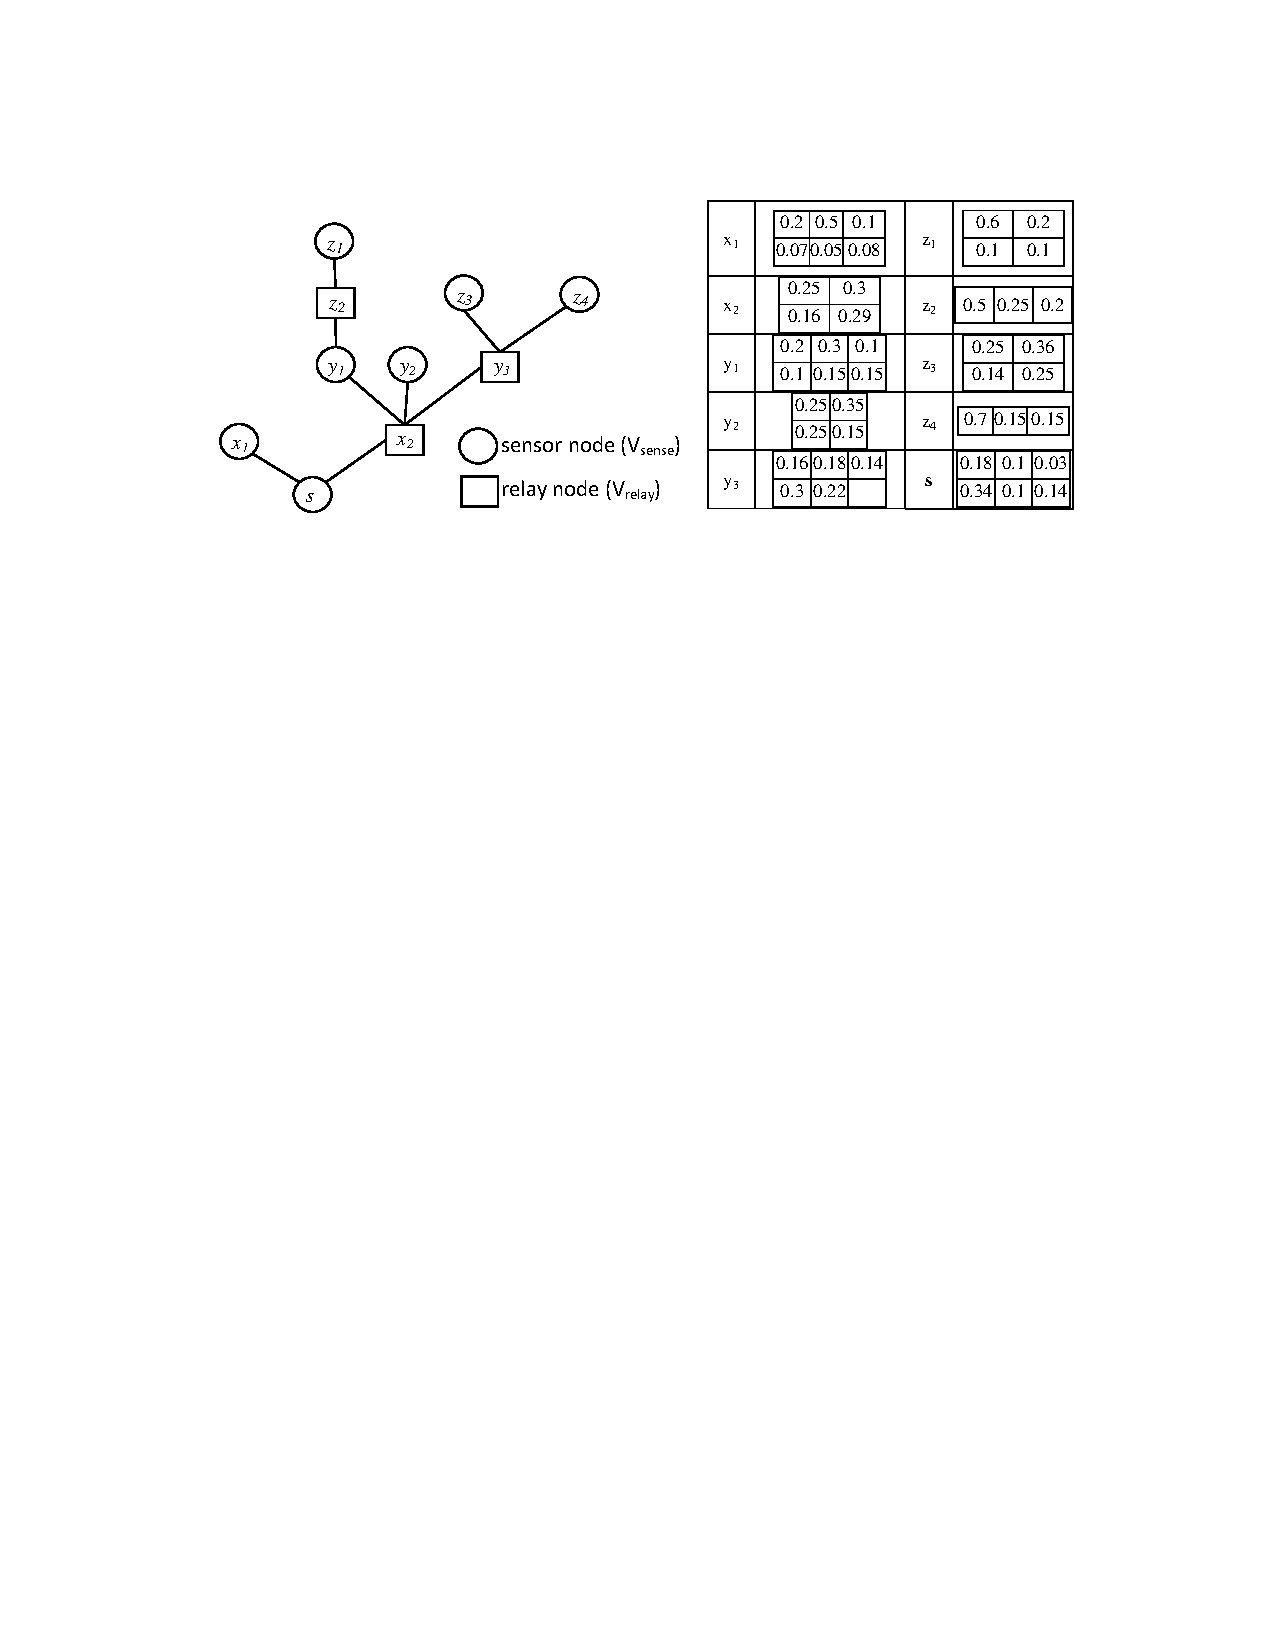
\includegraphics[width=4 in, height=1 in]{LocalitySet.pdf}
\caption{Network with Probabilistic locality set}
\end{figure}
\end{frame}
%------------------------------------------------

%------------------------------------------------
\begin{frame}
\frametitle{Node Reachability}
\begin{itemize}
\item node $x$ can reach node $y$ if the acoustic signal strength from $x$ to $y$ (and vice versa) exceeds a certain threshold value.
\item we set $E_G(x[i],y[j])= 1$ iff the two nodes $x$ and $y$ can reach each other if they are located anywhere in their respective rectangles $x[i]$ and $y[j]$.

\item connectivity between $x$ and $y$ is ignored if 
they can reach each other at some (but not all) pairs of points in their respective rectangles.

\item ignoring connectivity in such cases results
in computing lower bounds on the network connectivity, as required.
\end{itemize}
\end{frame}
%------------------------------------------------

\begin{frame}
\frametitle{Kinematic Model}
We note that this area is new to networking researchers where the obtained analytical
results are rooted in the mathematically deep field of fluid dynamics.
\begin{itemize}
\item A particle pathline is a path followed by an individual particle in a flow
\item A \textit{stream} function denoted  by $\psi$ measures the volume flow rate per unit depth.
\item Curves where $\psi$ is constant are called \textit{streamlines}
\end{itemize}
The stream function can be presented \\
\begin{equation}\label{eq:sf}
\psi(x,y,t)=-\tanh{[\frac{y-B(t)\sin(k(x-ct))}{\sqrt{1 + k^2 B^2(t) \cos^2(k(x-ct))}} ]} + cy
\end{equation}
 where $  B(t) = A + \epsilon \cos(\omega t)$  and the x and y velocities are given by
 
 \begin{equation}\label{eq:lf}
\dot{x}=-\frac{\partial \psi}{\partial y} ; \dot{y}=\frac{\partial \psi}{\partial x}
\end{equation}
\end{frame}
%------------------------------------------------
\begin{frame}
\frametitle{Kinematic Model (cont.)}
\vspace{-1em}
\begin{figure}[!htb]
\begin{minipage}[]{0.5\linewidth}
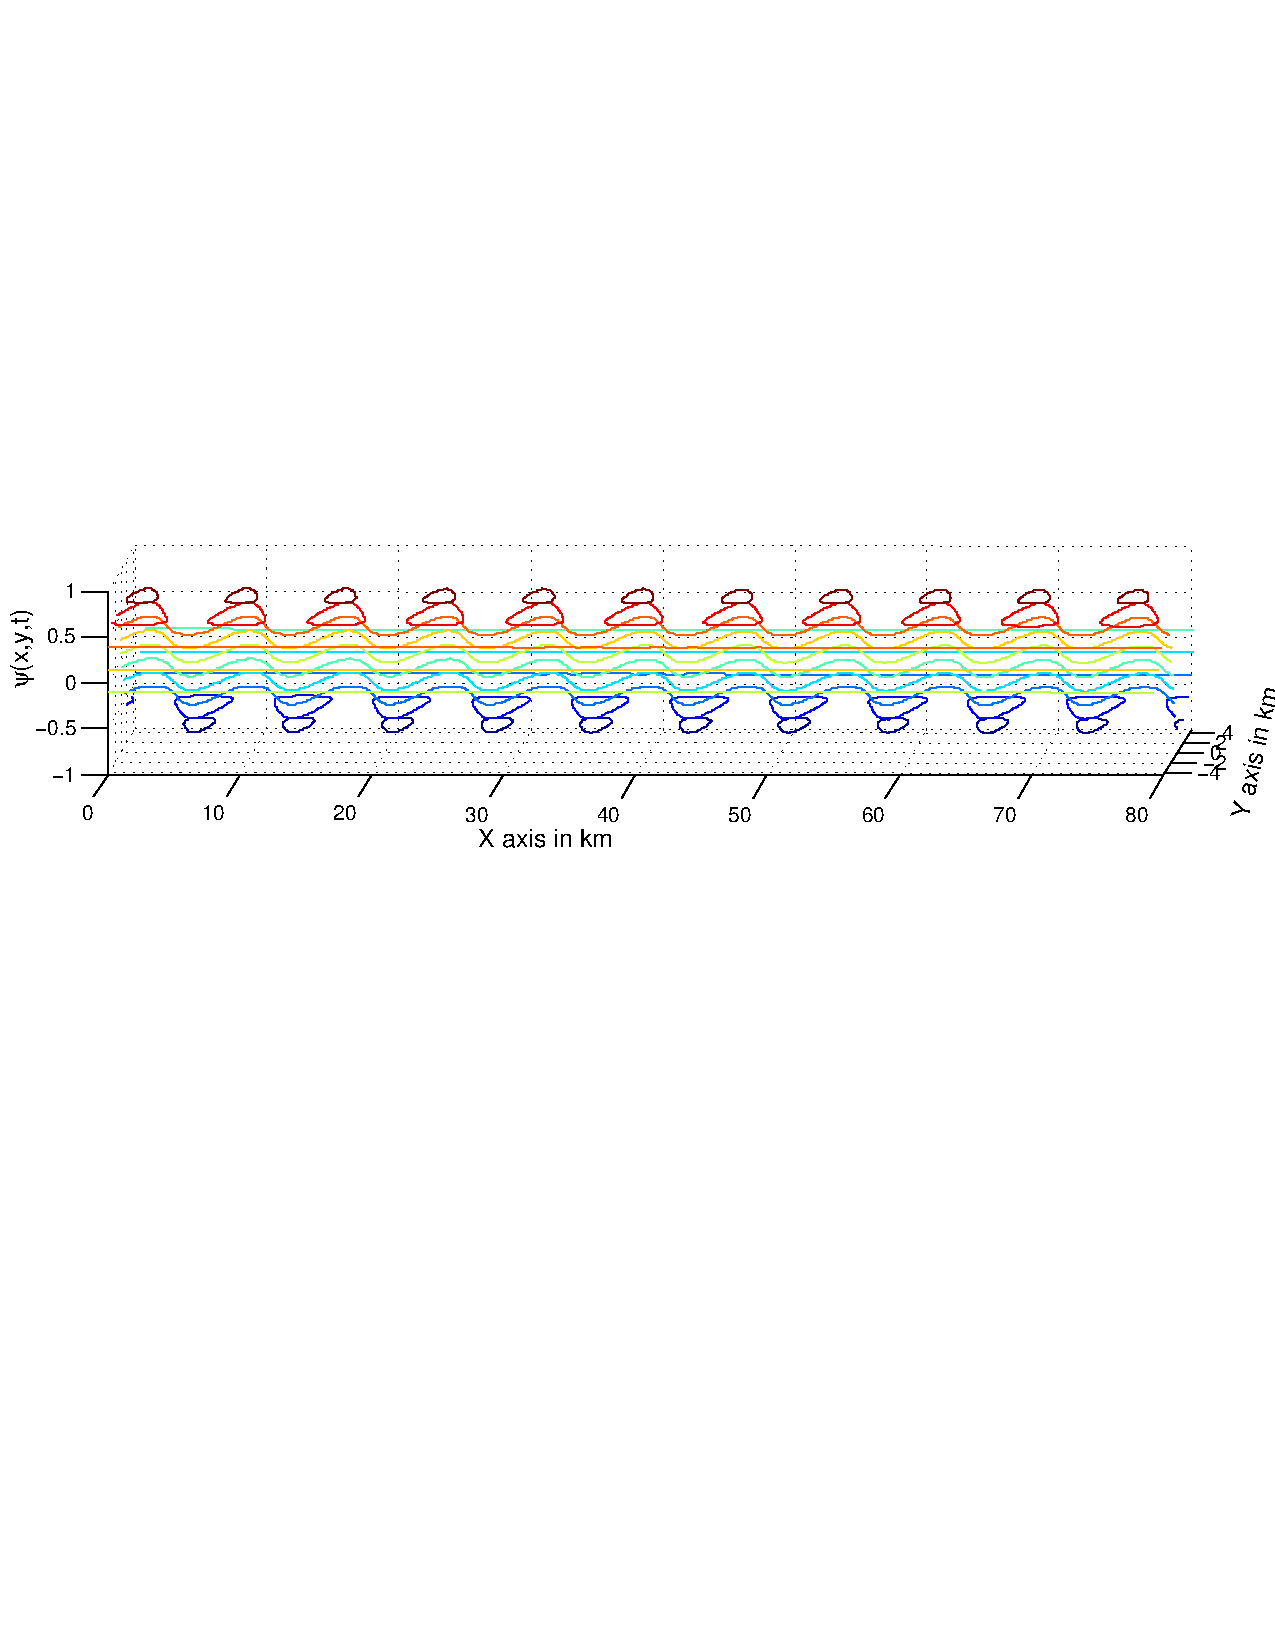
\includegraphics[width=2 in, height=1.5 in]{3D1.pdf}
\vspace{-1em}
 \caption{ A 3D plot of \ref{eq:sf}}
 \label{fig:kme3d}
 \end{minipage}
 \begin{minipage}{0.45\linewidth}
 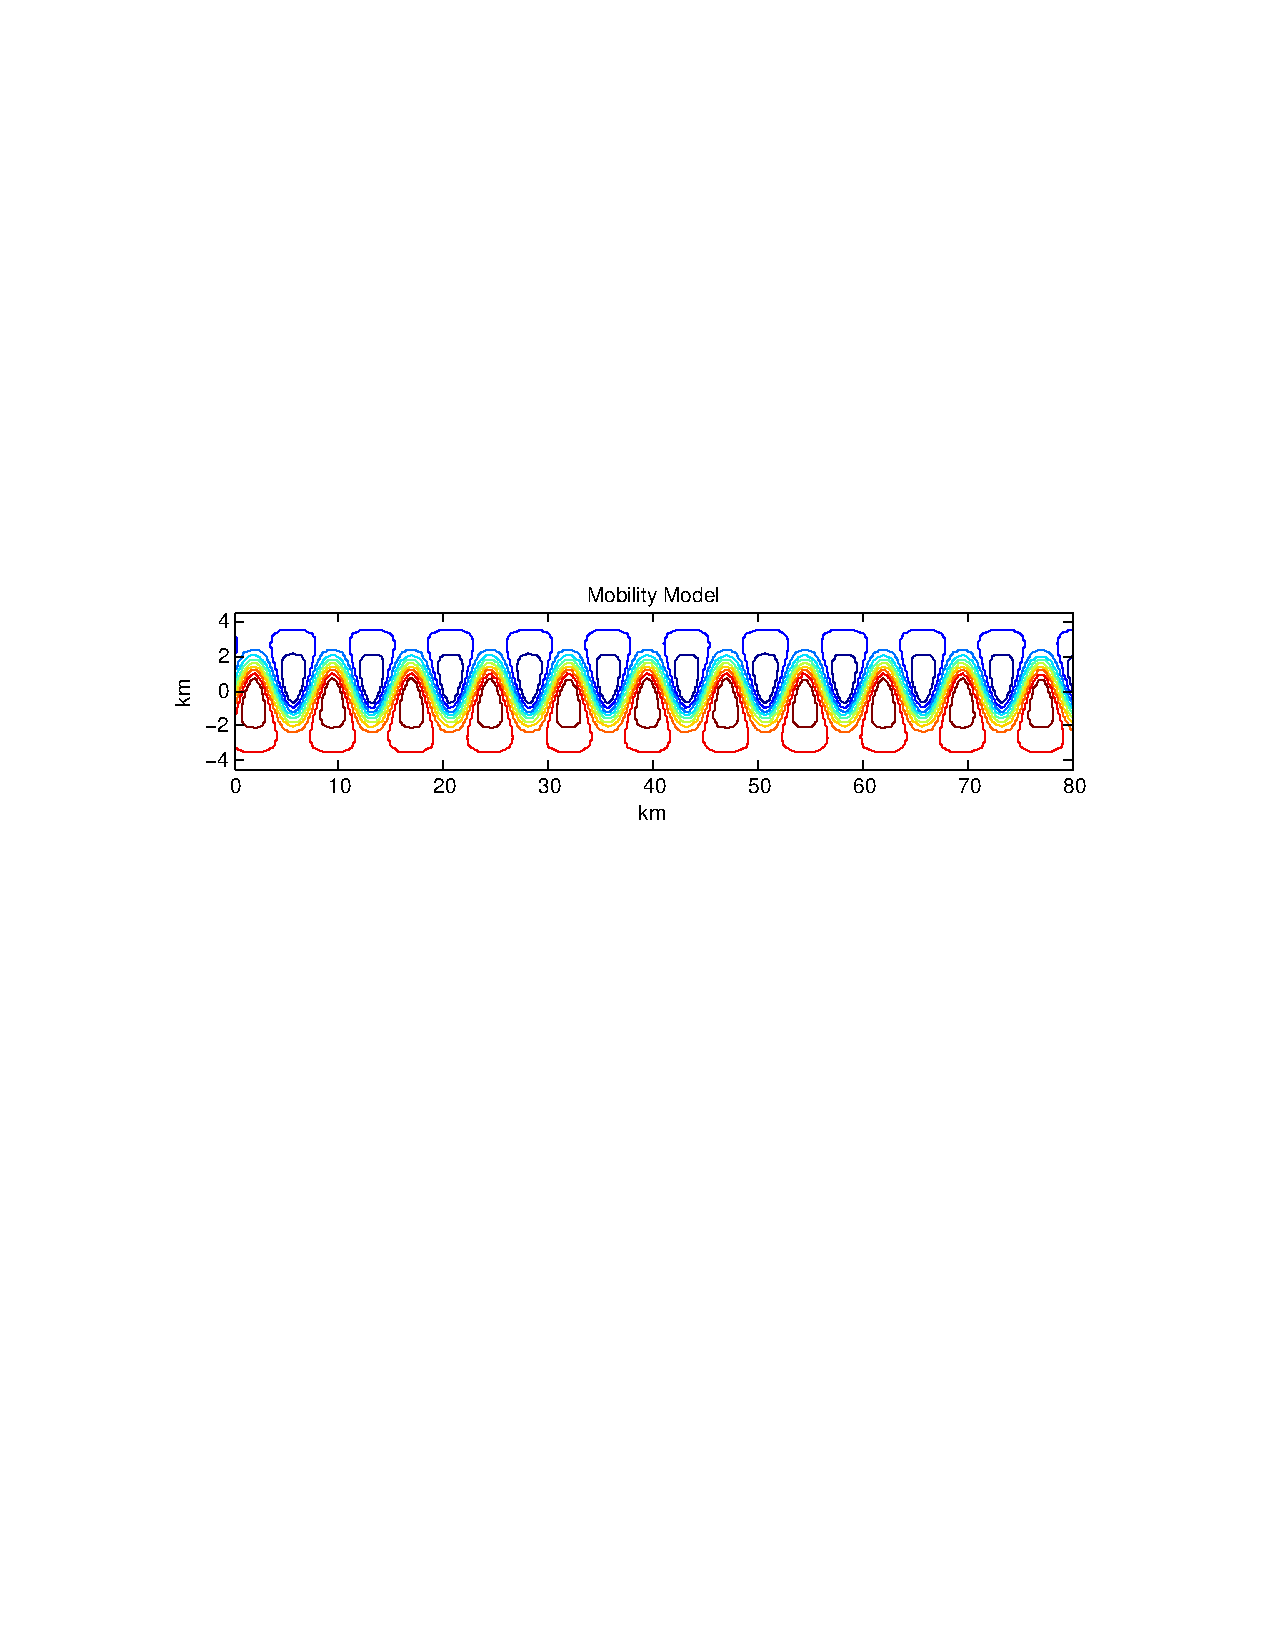
\includegraphics[width=2 in, height=1.5 in]{MCM.pdf}
 \vspace{-1em}
 \caption{ A plot of  \ref{eq:sf} at $t=0$.}
 \label{fig:kme}
 \end{minipage}
\end{figure}
\vspace{-1em}
\begin{figure}[!htb]
\begin{minipage}[]{.5\linewidth}
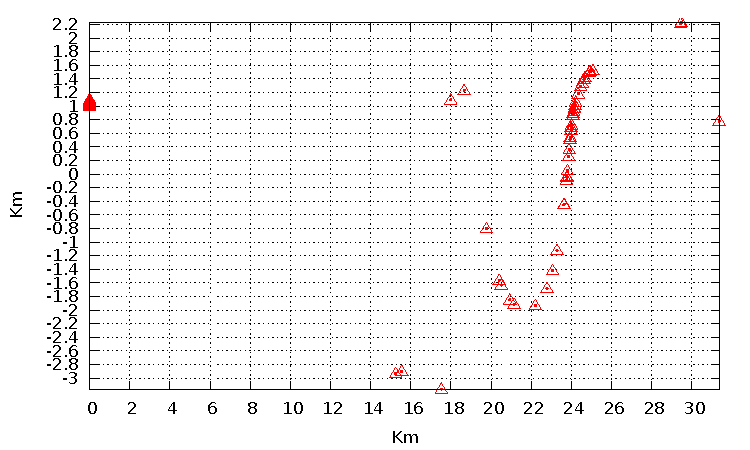
\includegraphics[width=2 in, height=1 in]{start_end_50.pdf}
\vspace{-1em}
 \caption{ Start and end points of 50 nodes}
\label{fig:res11}
\end{minipage}
\begin{minipage}{.45\linewidth}
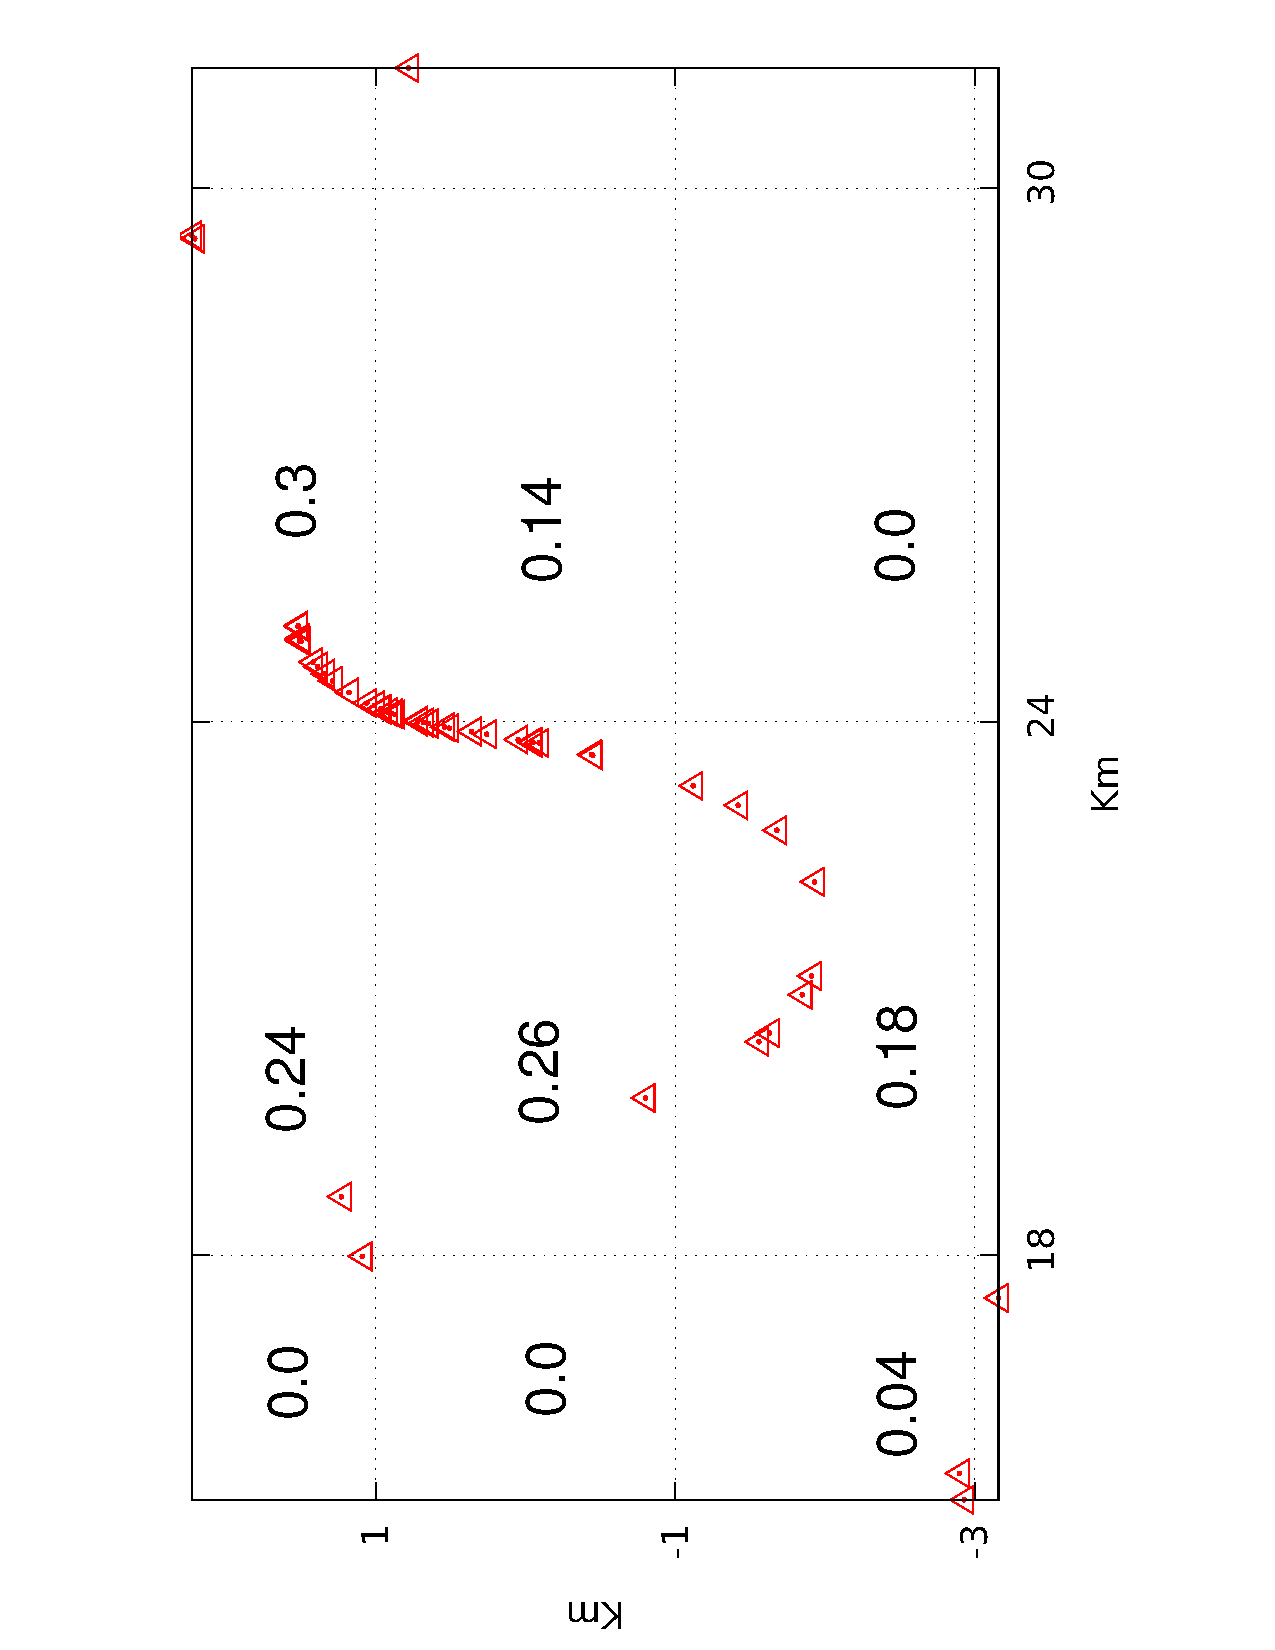
\includegraphics[width=1 in, height=1 in,angle=-90]{points1.pdf}
\vspace{-0.5em}
 \caption{probabilistic distribution}
\label{fig:ges11}
 \end{minipage}
\end{figure}
\end{frame}
%------------------------------------------------
%%\subsection{Problem Definition}
\begin{frame}
\frametitle{Problem Definition}
We define four probabilistic connectivity problem. They are 
\begin{itemize}
\item $\ACONN$ problem
\item $\ARCONN$ problem
\item $\SCONN$ problem
\item $\SRCONN$ problem
\end{itemize}
\end{frame}
%-----------------------------------------------
%-----------------------------------------------
\begin{frame}
\frametitle{the $\ACONN$ problem}
\begin{definition}[\textbf{the $A$-$CONN$ problem}]
\normalfont
Given a probabilistic network $G$ with no relay nodes, compute the probability $Conn(G)$ that the network is in a state where the sink node $s$ can reach all sensor nodes. 
\end{definition}
\begin{figure}
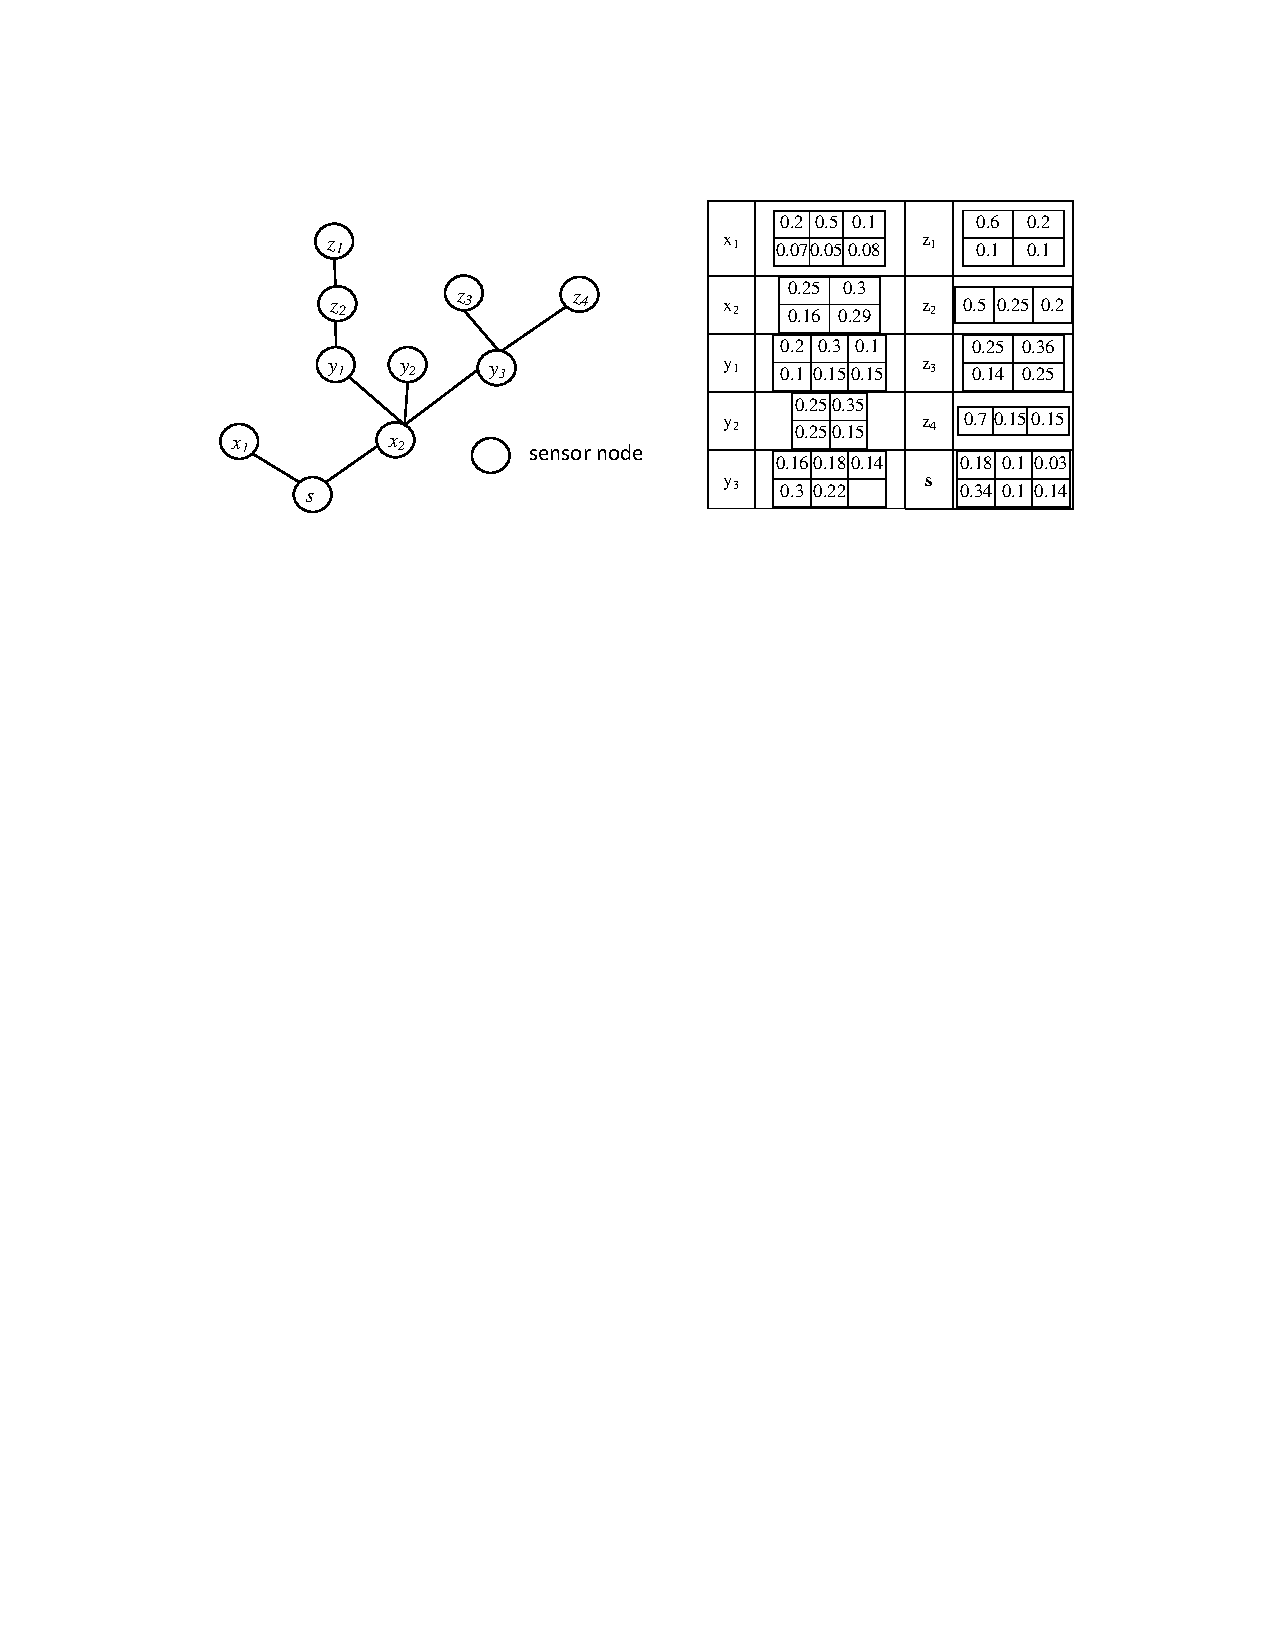
\includegraphics[width=4 in, height=1.5 in]{ACONN.pdf}
\caption{Network with Probabilistic locality set}
\end{figure}
\end{frame}
%---------------------------------------------------

%-----------------------------------------------

%-----------------------------------------------

%---------------------------------------------------

\begin{frame}
\frametitle{the $\ARCONN$ problem}
\begin{definition}[\textbf{the $AR$-$CONN$ problem}]
\normalfont
Given a probabilistic network $G$ where $V_{relay}$ is possibly non-empty, compute the probability $Conn(G)$ that the network is in a state where the sink node $s$ can reach all sensor nodes. 
\end{definition}

\begin{figure}
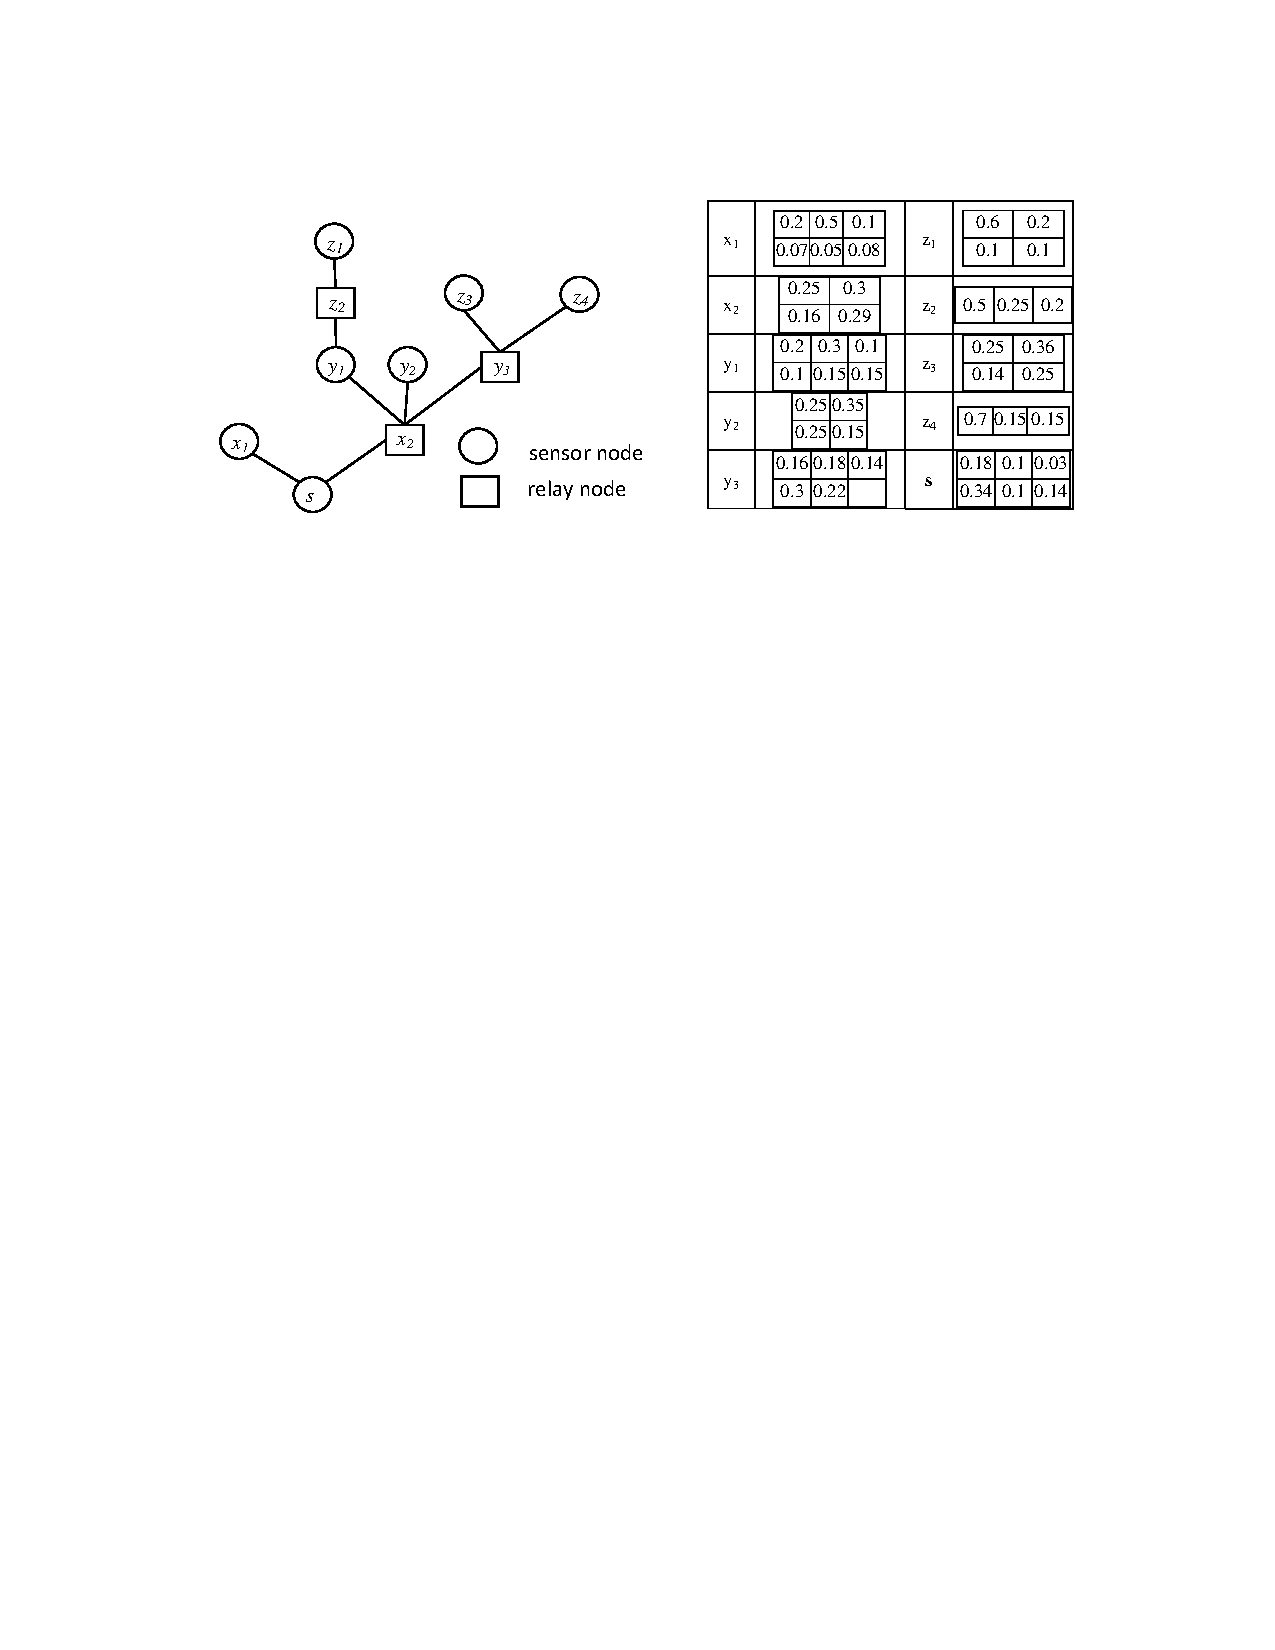
\includegraphics[width=4 in, height=1.5 in]{ARCONN.pdf}
\caption{Network with Probabilistic locality set with relay nodes}
\end{figure}
\end{frame}

%-----------------------------------------------
%-----------------------------------------------
\begin{frame}
\frametitle{the $\SCONN$ problem}

\begin{definition}[\textbf{the $S$-$CONN$ problem}]
Given a probabilistic network $G$ with no relay nodes, and a required number of sensor nodes $n_{req}\leq |V_{sense}|$, compute the probability $Conn(G,n_{req})$ that the network is in a state where the sink node $s$ can reach a subset of sensor nodes having at least $n_{req}$ sensor nodes. 
\end{definition}

\begin{figure}
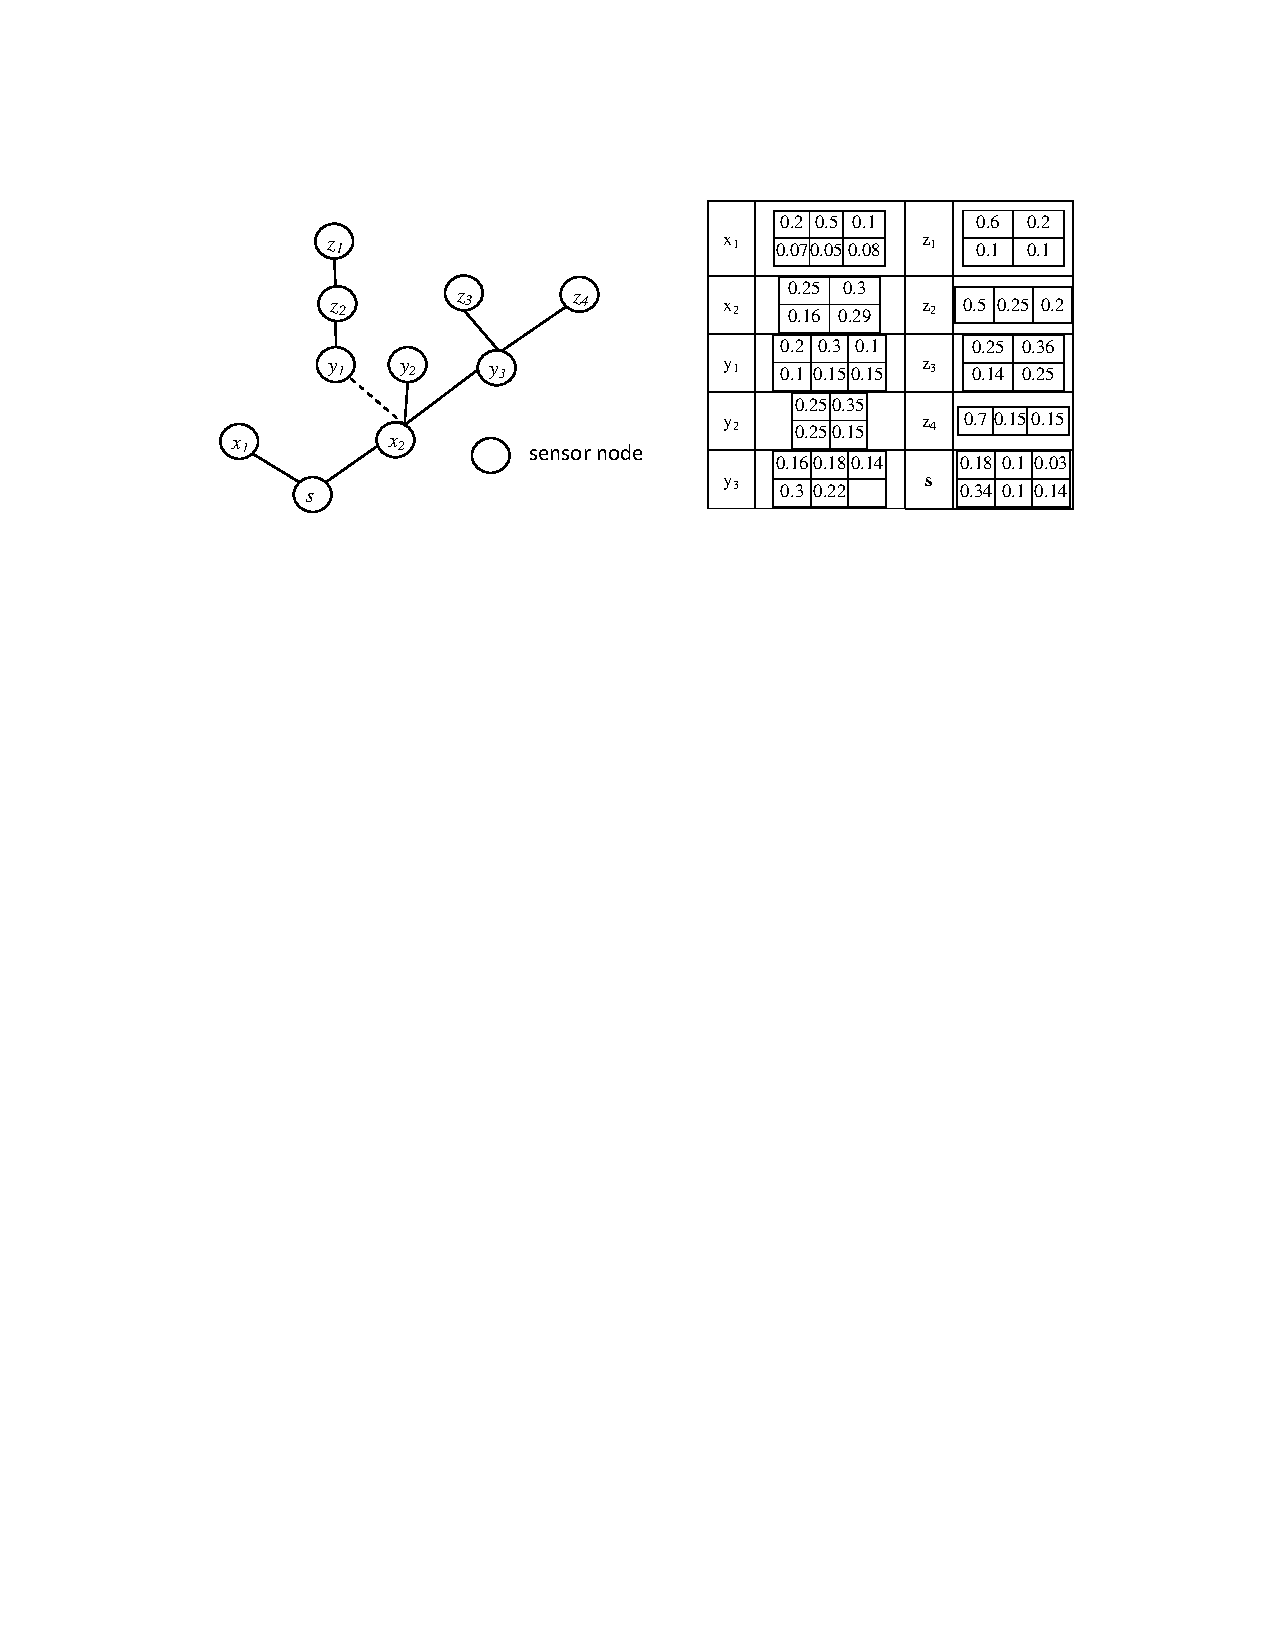
\includegraphics[width=4 in, height=1.5 in]{SCONN.pdf}
\caption{Network with Probabilistic locality set and $n_{req}=7$}
\end{figure}
\end{frame}
%------------------------------------------------

%-----------------------------------------------

%-----------------------------------------------
%------------------------------------------------
\begin{frame}
\frametitle{the $\SRCONN$ Problem}
\begin{definition}[\textbf{the $SR$-$CONN$ problem}]

Given a probabilistic network $G$ where $V_{relay}$ is possibly non-empty, and a required number of sensor nodes $n_{req}\leq |V_{sense}|$, compute the probability $Conn(G,n_{req})$ that the network is in a state where the sink node $s$ can reach a subset of sensor nodes having at least $n_{req}$ sensor nodes. 
\end{definition}

\begin{figure}
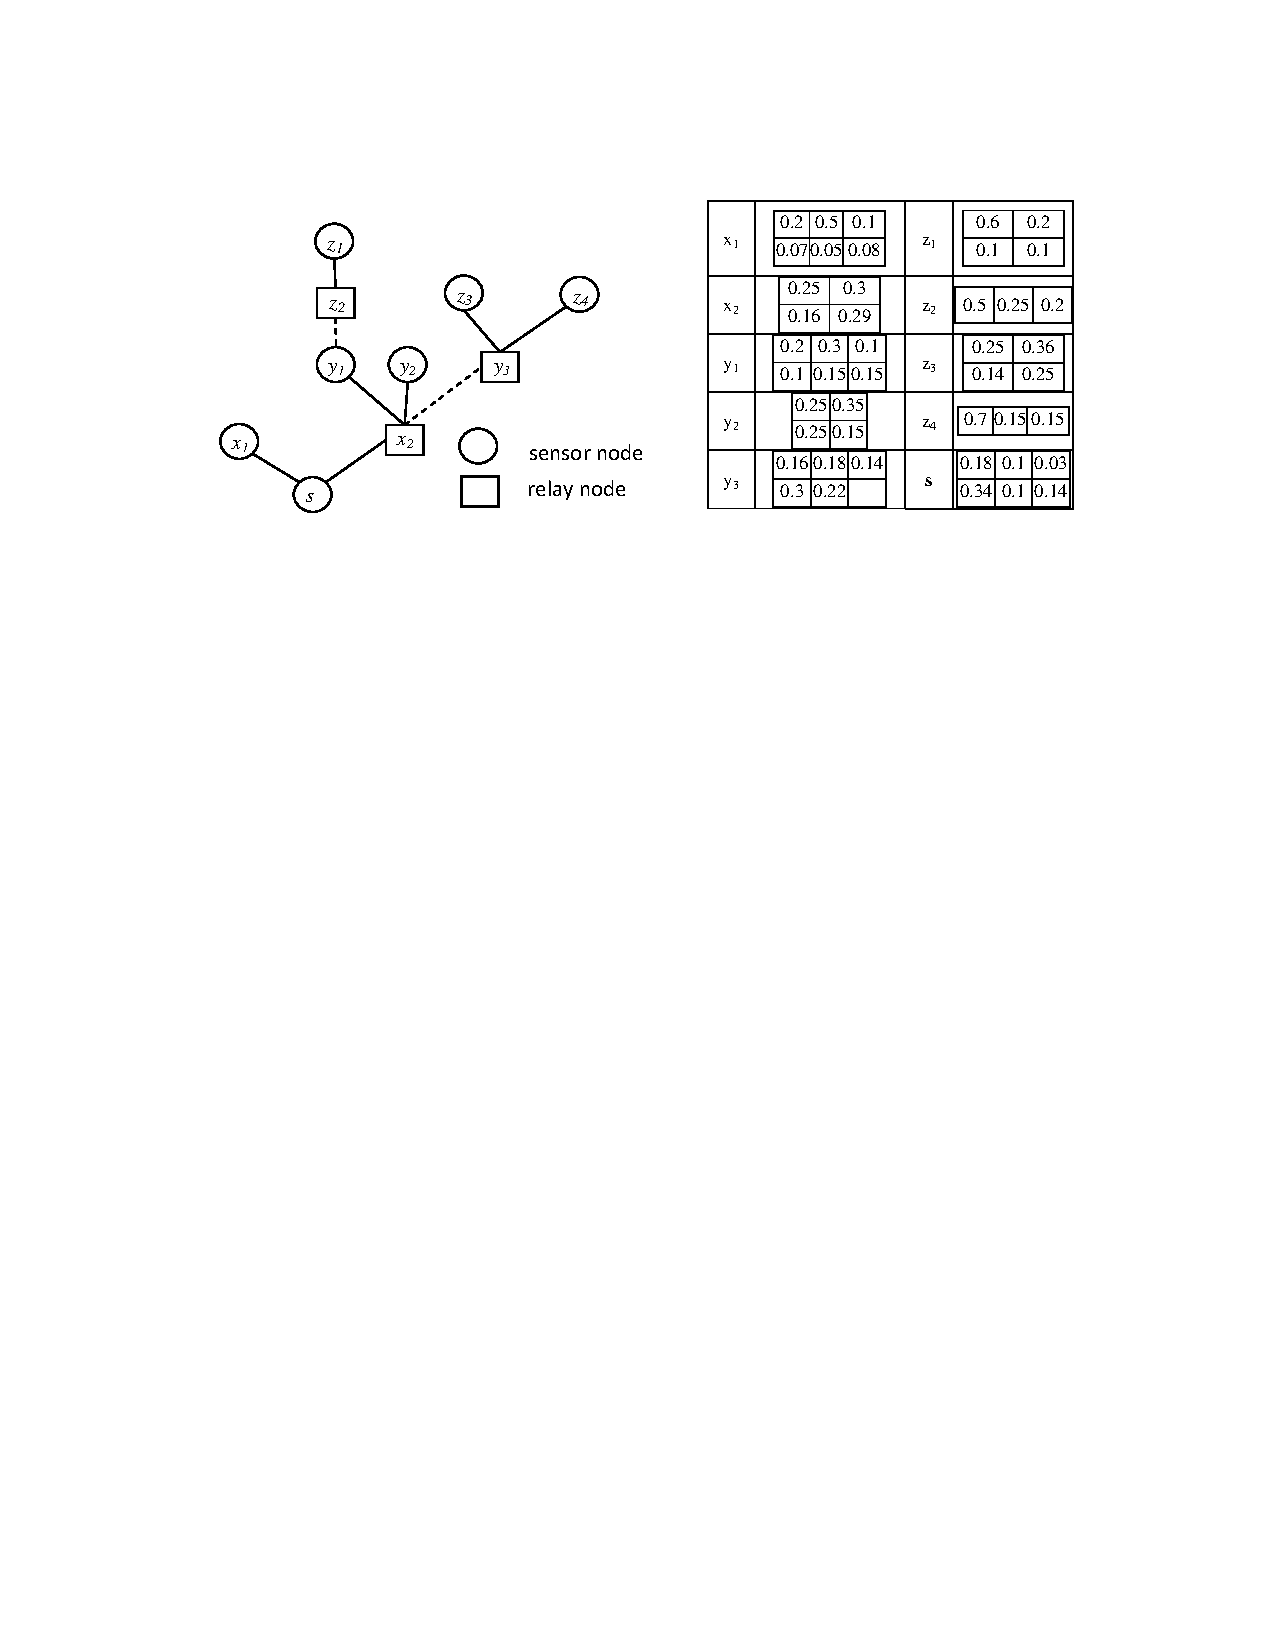
\includegraphics[width=4 in, height=1.5 in]{SRCONN.pdf}
\caption{Network with Probabilistic locality set and relay nodes where $n_{req}=4$}
\end{figure}
\end{frame}

%-----------------------------------------------

%-----------------------------------------------

\begin{frame}
\frametitle{Network State}
\begin{itemize}
\item A probabilistic graphs arises when network is in some particular network states.
\item A state $S$ of $V$ can be specified by $\{v_1[i_1], v_2[i_2], . . . , v_n[i_n]\}$
\item If locations are independent, we have $Pr(S) =\prod_{v_{\alpha}\in V} p_{v_\alpha[i_\alpha]}$.

\item In the $A$-$CONN$ and $AR$-$CONN$ problem, a state is \textbf{operating} if the
sink $s$ can reach all sensor nodes in $V_{sense}$ . 
\item Similarly, in the $S$-$CONN$ and $SR$-$CONN$ problem, a state $S$ is \textbf{operating} if the sink node $s$ can reach a $n_{req}$ sensor
nodes.
\end{itemize}
\vspace*{-0.5 cm}
\begin{columns}
\vspace*{-0.5 cm}

\column{0.8\linewidth}
\begin{figure}[h]
\centering
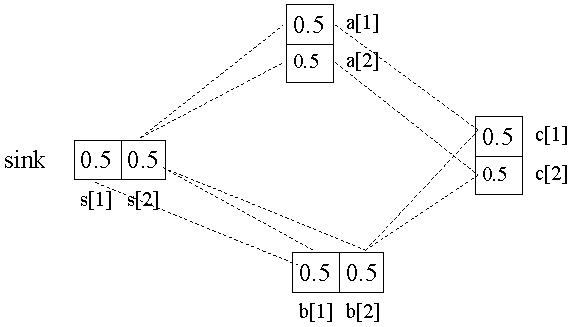
\includegraphics[width=1.8 in, height=1 in]{Figure1.pdf}
\vspace*{-0.5 cm}
 \caption{ An example network}
\end{figure}
\end{columns}
\end{frame}
%------------------------------------------------
%\subsection{Thesis Contribution}
\begin{frame}
\frametitle{Thesis Contribution}
An efficient dynamic programming algorithms
\begin{enumerate}
\item for the $\SRCONN$ problem on probabilistic networks whose underlying graphs are trees.% The algorithm solves the more restricted $\ARCONN$ problem with little overhead compared to a dedicated algorithm to solve the $\ARCONN$ problem.
\item for the $\ACONN$ problem on partial $k$-trees.
\item for the $\ARCONN$ and $\SRCONN$ problems on partial $k$-trees.
\end{enumerate}
All cases the algorithm runs in polynomial time for any fixed $k$. 
\end{frame}
%------------------------------------------------
\section{Overview on $k$-Trees and Partial $k$-Trees}
%------------------------------------------------

\begin{frame}
\frametitle{$k$-Trees and Partial $k$-Trees}
\vspace{-0.7em}
\begin{definition} For a given integer $k\geq 1$, the class of $k$-trees is defined as follows
\begin{enumerate}
\item A $k$-clique is a $k$-tree.
\item If $G_n$ is a $k$-tree on $n$ nodes then the graph $G_{n+1}$ obtained by adding a new node adjacent to every node in $k$-clique of $G_n$. 
\end{enumerate}
\end{definition}
\vspace{-1em}
\begin{figure}[!htb]
\begin{minipage}[]{0.4\linewidth}
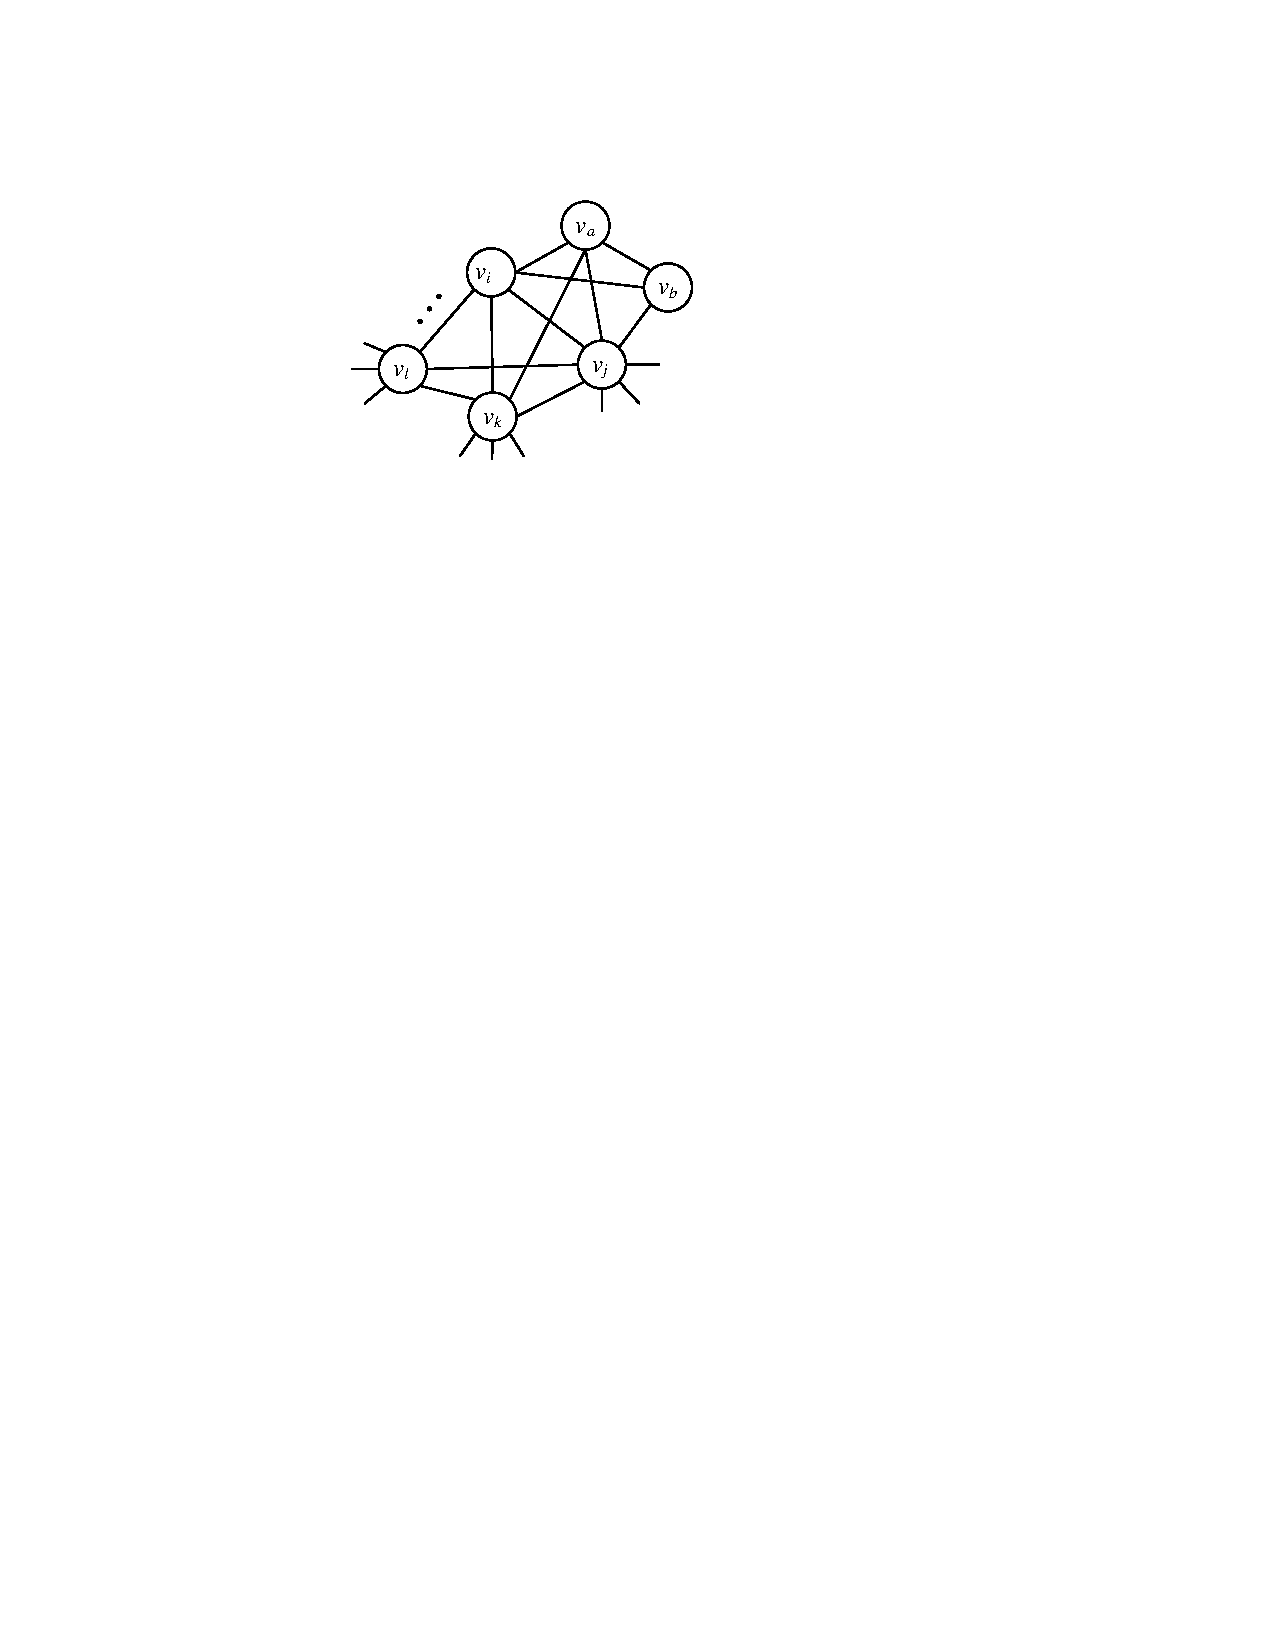
\includegraphics[width=1 in, height=.8 in]{Ch3f2.pdf}
\vspace{-1em}
 \caption{a fragment of a 3-tree}
 \label{fig:f3t1}
 \end{minipage}
 \begin{minipage}{0.45\linewidth}
 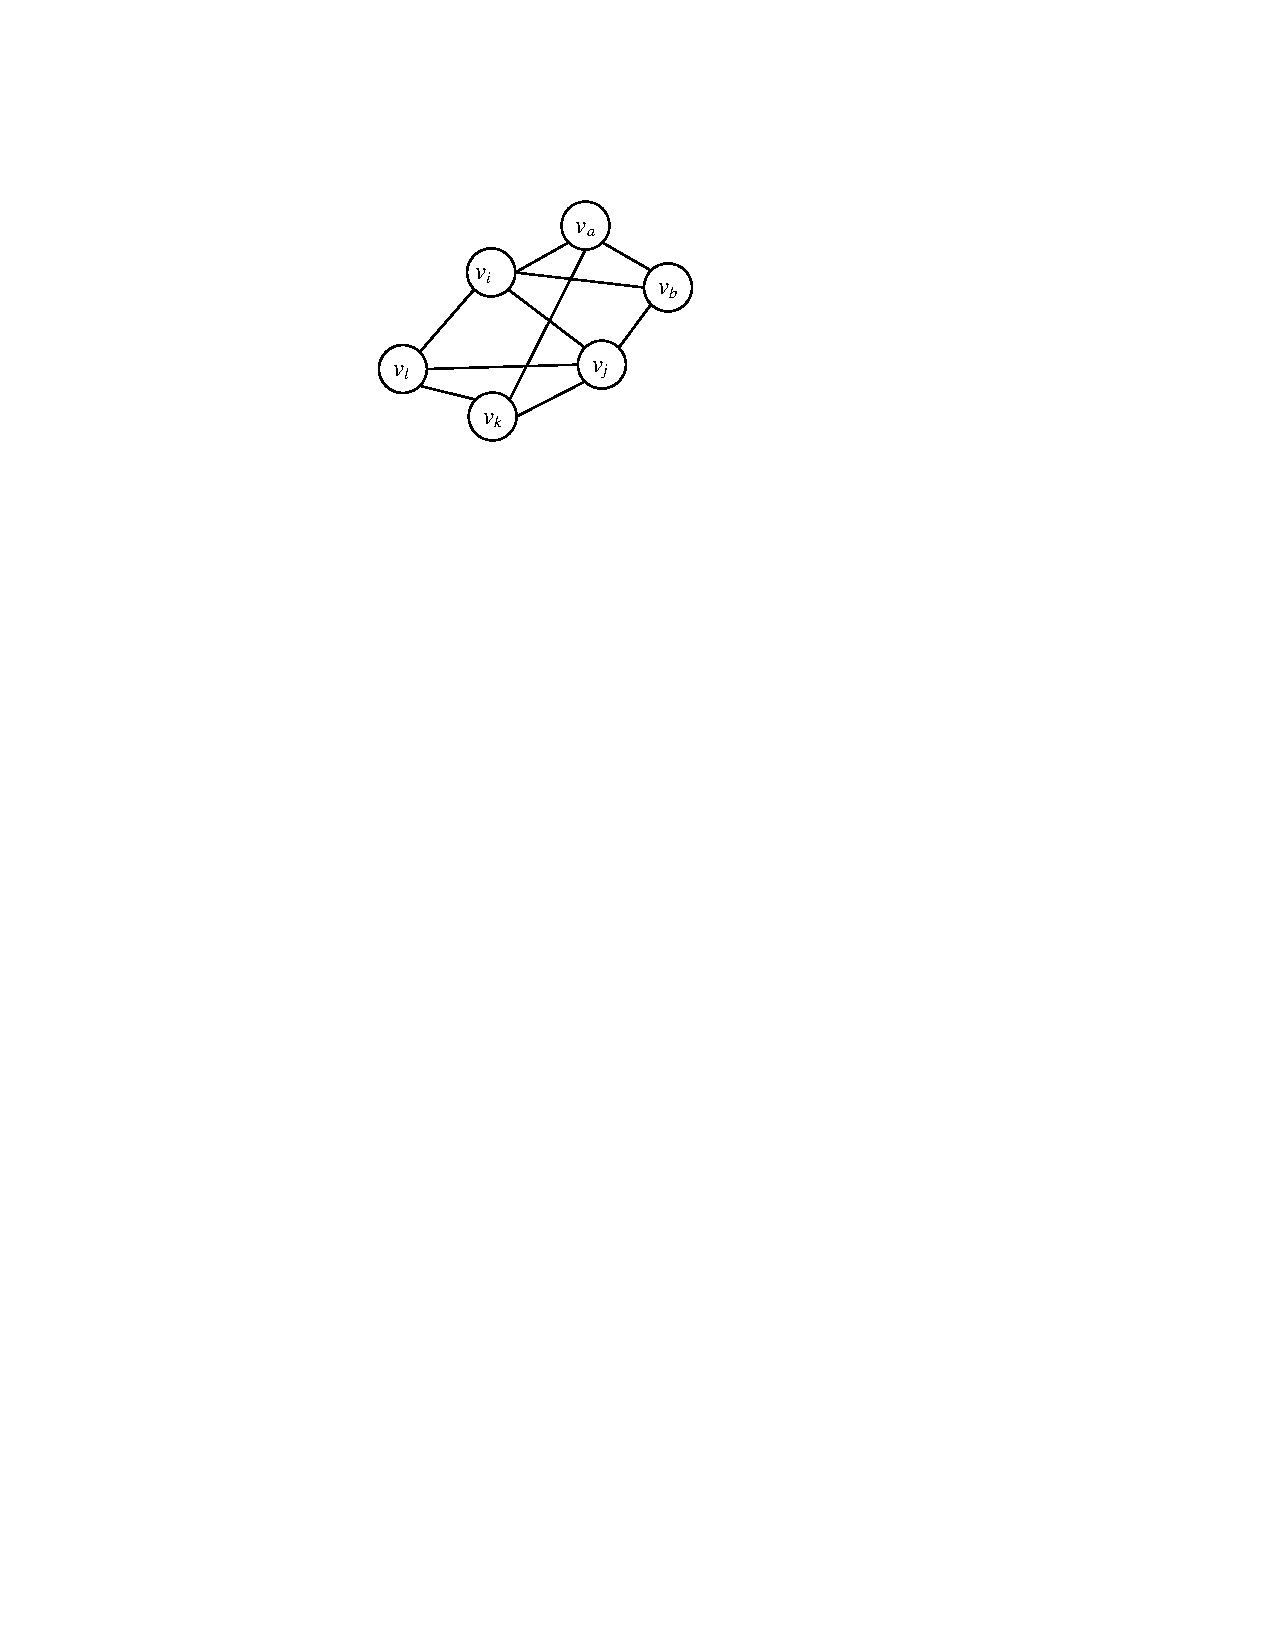
\includegraphics[width=1 in, height=0.8 in]{Ch2f2.pdf}
  \vspace{-1em}
 \caption{a fragment of partial 3-tree}
 \label{fig:f3t2}
 \end{minipage}
\end{figure}
\vspace{-1em}
A partial $k$-tree is a $k$-tree possibly missing some edges
and a \textit{$k$-perfect elimination sequence} $(k\mbox{-}PES)$ of  $G$ is an ordering $(v_1,v_2,\ldots,v_r)$ of $v(G)$
\vspace{-0.5em}
\begin{example}
\normalfont 
For the graph $G$ in figure , $(v_a,v_b,v_i,v_j,v_k,v_l)$ is a 3-$PES$. 
\end{example}
\end{frame}
%%------------------------------------------------
%%\subsection{Graphs with Bounded Tree-width}
%%------------------------------------------------
%\begin{frame}
%\frametitle{Graphs with Bounded Tree-width}
%\begin{definition}\normalfont 
%A \textit{tree-decomposition} of a graph $G$ is a family ($X_i:i\in I$) of subsets of $V(G)$, together with a tree $T$ with $V(T)=I$, with the following properties.
%\begin{enumerate}
%\item $\displaystyle \bigcup_{i\in I} X_i =V(G)$.
%\item Every edge of $G$ has both its ends in some $X_i$.
%\item For $i,j,k \in I$, if $j$ lies on the path of $T$ from $i$ to $k$ then $X_i\cap X_k \subseteq X_j$. 
%\end{enumerate} 
%\end{definition}
%The \textit{width} of a tree-decomposition is $max(|X_i|-1:i\in I)$. 
%The \textit{tree-width} of $G$ is the minimum $w \geq 0$ such that $G$ has a tree-decomposition of width $\leq w$. 
%
%\end{frame}
%%------------------------------------------------
%%\subsection*{Tree Decomposition example}
%%------------------------------------------------
%\begin{frame}
%\frametitle{Tree Decomposition example}
%\begin{example}
%\normalfont
%Figure \ref{fig:GandT}(a) illustrates a graph $G$ having a tree-decomposition shown in figure \ref{fig:GandT}(b). The width of the tree decomposition is 3. One may verify that 3 is actually the tree-width of $G$. 
%\end{example}
%\begin{figure}[!htb]
%\centering
%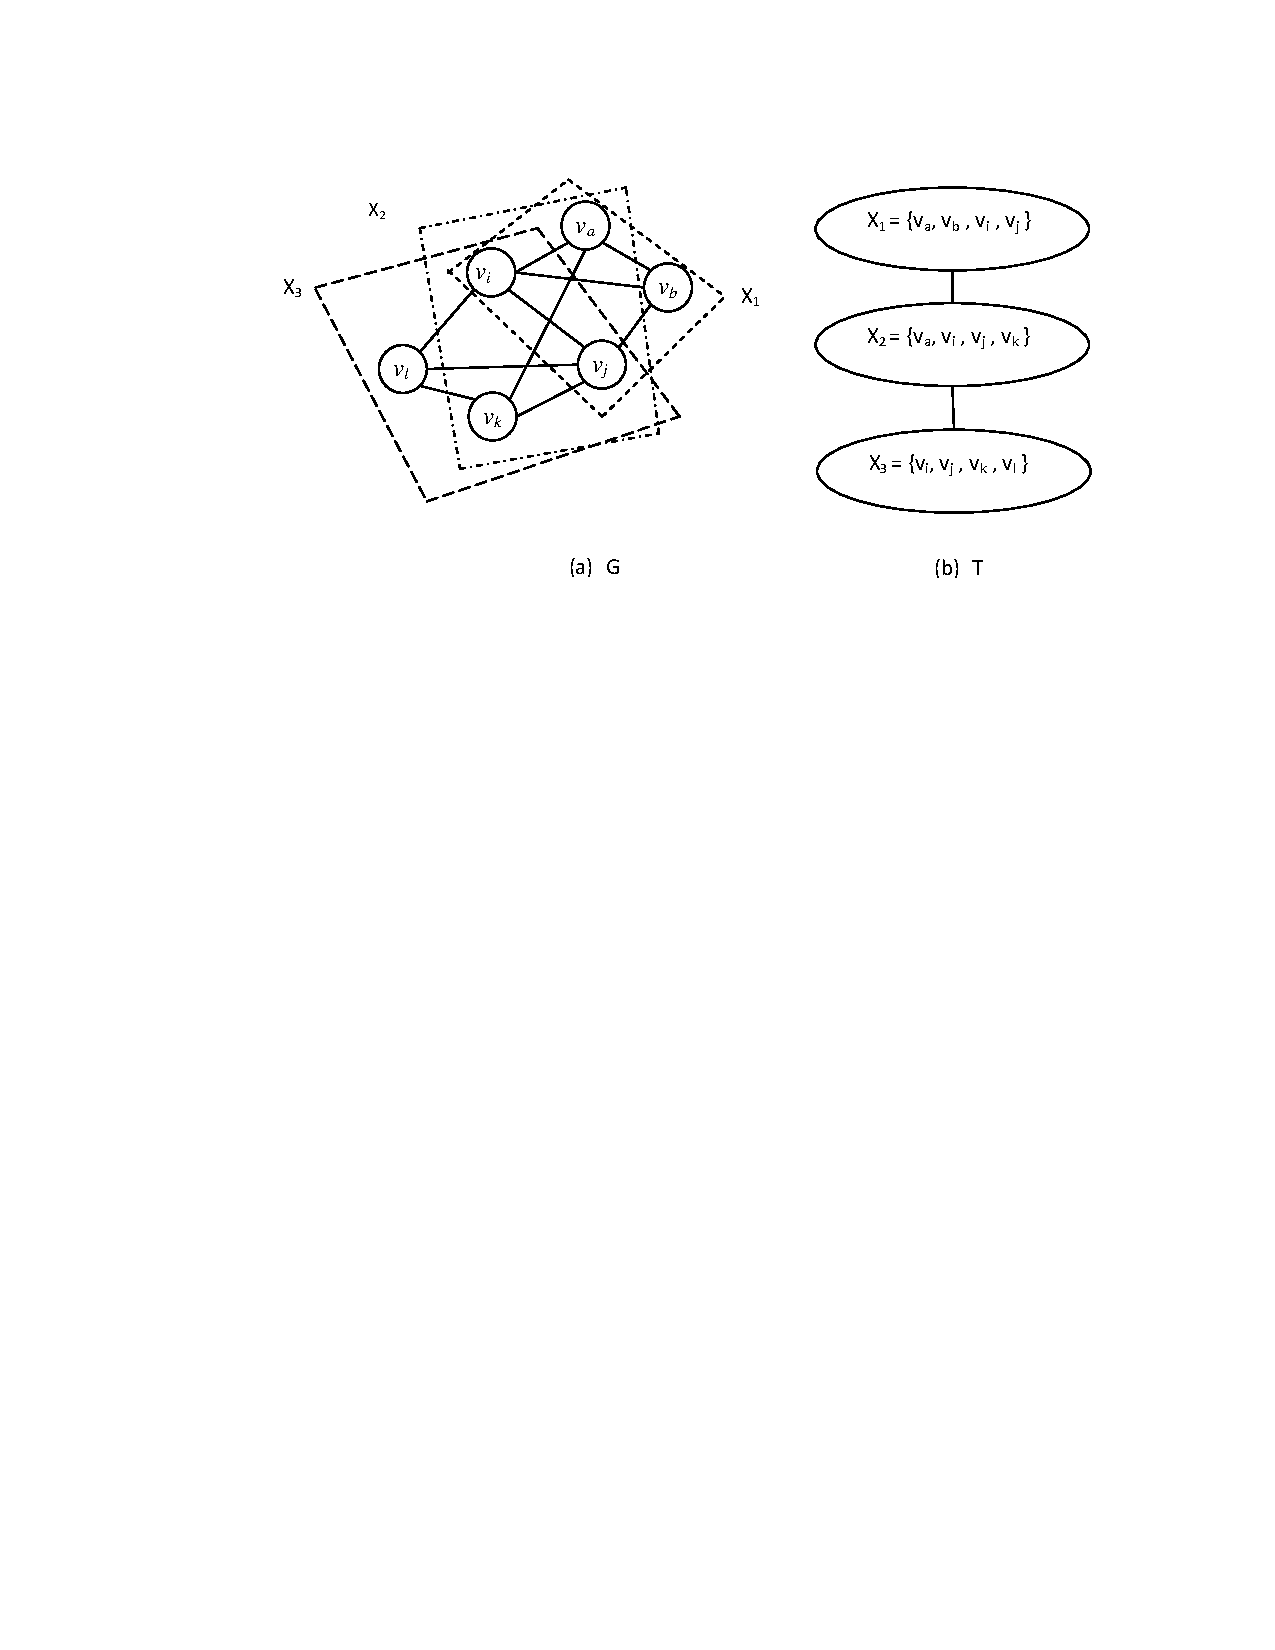
\includegraphics[width=3 in, height=1.2 in]{Ch2f3.pdf}
% \caption{ Tree decomposition}
% \label{fig:GandT}
%
%\end{figure}
%\end{frame}
%------------------------------------------------
%\subsection{Dynamic Programing on Partial $k$-Trees}
%------------------------------------------------
\begin{frame}
\frametitle{Dynamic Programing on Partial $k$-Trees}
We inspired by Wald and Colbourn 1983 dynamic programming algorithm for solving the Steiner tree problem on partial 2-trees where each edge $\alpha = (x, y)$ of $G$ associates six cost measures, which summarize the cost incurred so far of the subgraph $S$ which has been reduced onto the edge $(x , y )$
\begin{enumerate}
\item $st(\alpha)$ is the minimum cost of a Steiner tree for $S$, in which $x$ and $y$ appear in the same tree.
\item $dt(\alpha)$ is the minimum cost of two disjoint trees for $S$ including all targets, one tree involving $x$ and the other $y$.
\item  $yn(\alpha)$ is the minimum cost of a Steiner tree for $S$, which includes $x$ but not $y$.
\item $ny(\alpha)$ is the minimum cost of a Steiner tree for $S$, which includes $y$ but not $x$.
\item $nn(\alpha)$ is the minimum cost of a Steiner tree for $S$, which includes neither $x$ nor $y$.
\item $none(\alpha)$ is the cost of omitting all vertices of $S$ from a Steiner tree.
\end{enumerate}
\end{frame}

%A Steiner tree can be defined as follows.
%\begin{definition}
%Given a graph $G = (V,E)$ with positive integer edge costs, and a set of target nodes $V_{target}\subseteq V$, a Steiner tree, denoted $ST(G,V_{target} )$, is a subtree $G' = (V',E')$ satisfying
%\begin{enumerate}
%\item  $V_{target} \subseteq V'\subseteq V$ ,
%\item the sum of edge costs in $E'$ is minimum over all subtrees satisfying (1). 
%\end{enumerate}
%
%\end{definition}
%\vspace*{-0.15 cm}
%\begin{figure}
%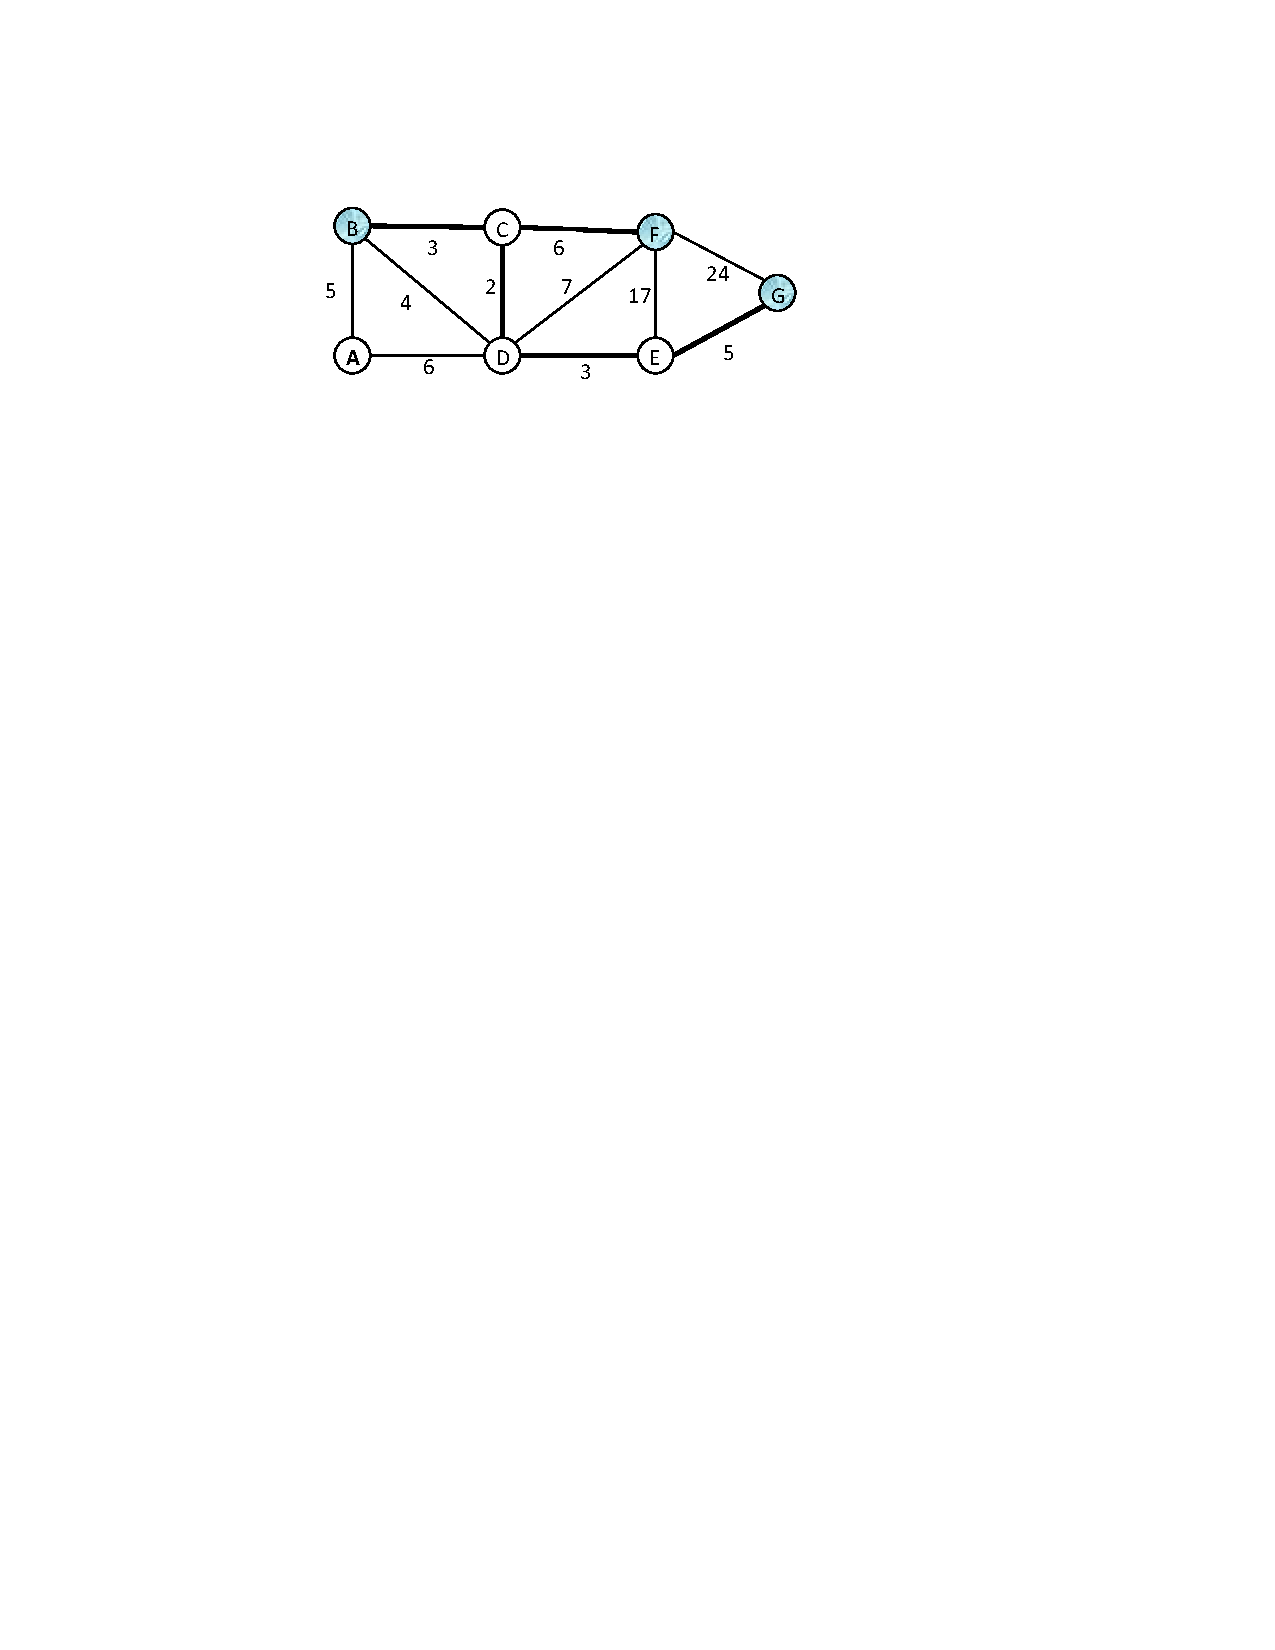
\includegraphics[width=3 in, height=1 in]{Steiner.pdf}
%\caption{A Steiner Tree}
%\end{figure}
%\end{frame}
%%------------------------------------------------
%%\subsection{Solving Steiner tree problem on partial 2-tree}
%
%%------------------------------------------------
%\begin{frame}
%\frametitle{Solving Steiner tree problem on partial 2-tree}
%
%In wald and colbourn 1983 devised algorithm, 
%------------------------------------------------
%\subsection{Our Approach}
%------------------------------------------------
\begin{frame}
\frametitle{Our Approach}
\begin{itemize}
\item  Store the six measures associated with edge $\alpha=(x,y)$ in a table, denoted $T_{x,y}$.
\item  The table provides key-value mappings. 
\item The keys replace the use of some of the names $st,dt,yn, $ etc. with set notation.
\item Not all names correspond to keys in this formulation.
\end{itemize}
 
Examples of names that correspond to keys are:

$st=\{x,y\}_1,dt=\{x\}_1\{y\}_1, yn=\{x\}_1\{y\}_0, \mbox{ and } ny=\{x\}_0\{y\}_1$.

\end{frame}
%------------------------------------------------
%\subsection{Set Partitions}
%------------------------------------------------
\begin{frame}
\frametitle{Set Partitions}
\begin{itemize}
 \item Given a set $X$, a partition of $X$ is a set $\{X_1,X_2,\ldots, X_r\}$, $1\leq r\leq |X|$ such that 
\begin{enumerate}
\item $X=\displaystyle \bigcup_{i=1,2,\ldots,r} X_i$.
\item The $X_i$s are pairwise disjoint.
\end{enumerate}
\item In our algorithm, $X$ is a set of nodes in a $k$-clique, and the partition of $X$ are used as part of states of dynamic programs.
\item The number of all possible partition of a set $X$ on $n$ elements are known as Bell numbers, denoted $B_n$.
\item The first few Bell numbers are 
\begin{center}
$\begin{array}[t]{l}
B_0=B_1=1,B_2=2,B_3=5,B_4=15,\\
B_5=52,B_6=203,B_7=877,B_8=4140, \ldots \\
\end{array}$
\end{center}
\item Bell numbers satisfy the following recurrence equation:
\begin{center}
$ B_0=1, B_1=1 \mbox{ and } B_{n+1}=\displaystyle \sum_{k=0}^n (\begin{array}{l} n \\ k \end{array})B_k.
$
\end{center}
\end{itemize}
\end{frame}
%------------------------------------------------
%%\subsection{Recognizing and Edge deletion problem on Partial $k$-tree}
%%------------------------------------------------
%\begin{frame}
%\frametitle{Recognizing and Edge deletion problem on Partial $k$-tree}
%\begin{enumerate}
%\item {\bf Recognizing  Partial $k$-Trees:} Given a graph $G$, and an integer $k\geq 1$, is $G$ a partial $k$-tree?\\
%\begin{itemize}
%\item The work of arnborg1987 shows $O(n^{k+2})$ algorithm for solving the problem if $k$ is fixed. 
%\item If $k$ is not fixed, then arnborg1987 shows that the problem is NP-complete.
%
%\item For any fixed  $k$, the work of bodlaender1993 improves on the above result by showing a linear time recognition algorithm.
%\end{itemize}
%The above results produce also a $k$-$PES$ if one exists.
%\nwline
%\item {\bf Edge Deletion Problem (EDP) to Obtain a Partial $k$-Tree:}  Given a graph $G$, and an integer $k$, find the minimum number of edges whose deletion gives a partial $k$-tree.
%\begin{itemize}
%\item For $k=1$, the problem is simple.
%\item For $k\geq 2$, the problem is NP-complete (From the work of elmallah1988 and the references therein)
%\end{itemize}
%\end{enumerate}
%
%\end{frame}
%%------------------------------------------------
%\subsection{The Random and Greedy Method}
%------------------------------------------------
\begin{frame}
\frametitle{The Random and Greedy Method}
\begin{columns}[t] 
\column{.65\textwidth}
\textbf{The Random Method.}
\begin{itemize}
\item {\bf Case $k=1$.} Choose any spanning tree.
\item {\bf Case $k=2$.} 
\begin{itemize}
\item Choose a spanning tree $G'\subseteq G$.
\item Fix an ordering of the remaining edges not in $G'$.
\item  For each edge $e$ in the fixed order, test whether $G'+e$ is a partial 2-tree.
\item  If yes, add $e$ to $G'$, and proceed to the next edge in the fixed order.
\end{itemize}
\item {\bf Case $k=3$.}
\begin{itemize}
\item Build a partial 2-tree $G'\subseteq G$.
\item Fix an ordering of the edges not in $G'$. 
\item For each edge $e$, test whether $G'+e$ is a partial 3-tree.
\item If yes, add $e$ to $G'$, and proceed to the next edge in the fixed order.
 \end{itemize}
\end{itemize}
\column{0.35\textwidth}
\textbf{The Greedy Method.}
\begin{itemize}
\item {\bf Case $k=1$:} Choose a minimum spanning tree.
\item {\bf Case $k=2$ and $3$:} As in cases $k=2$ and $3$, respectively, of the random method, where we sort the remaining edges in a non-decreasing order of their costs to obtain the fixed order
\end{itemize}
\end{columns}
\end{frame}

\section{Probabilistic Connectivity of Tree Network}
%\subsection{Notation and Definition}
%\subsection{Pseudo-code for $\SRCONN$ problem on tree network}
%\subsection{Running time Analysis}
\begin{frame}
\frametitle{Probabilistic Connectivity of Tree Network}
\begin{itemize}
\item Notation and Definition
\item Pseudo-code for $\SRCONN$ problem on tree network
\item Running time Analysis
\end{itemize}
\end{frame}
\begin{frame}
\frametitle{Notation and definition}
\begin{columns}[t]
\column{0.65\textwidth}
\vspace{-1.7em}
\begin{itemize}
\item	$type(x)$: $type(x)= 0$ and 1 if $x$ is a relay node and 
 a sensor node respectively.

\item	$n_{sense}(X)$: \# of sensor nodes in a given subset  of nodes $X\subseteq V$.

\item   $n_{relay}(X)$: \# of relay nodes in a given subset of nodes $X\subseteq V$.

\item $n(X)=n_{sense} + n_{relay}$.

\item $n_{sense,min}(X)$: The minimum number of sensor nodes in a given subset $X\subseteq V$. So,\\
\centerline{
$n_{sense,min}(X)=max(0,n_{req}-n_{sense}(\overline{X}))$
}
\end{itemize}
\column{0.35\textwidth}
\begin{figure}[!htb]
\centering
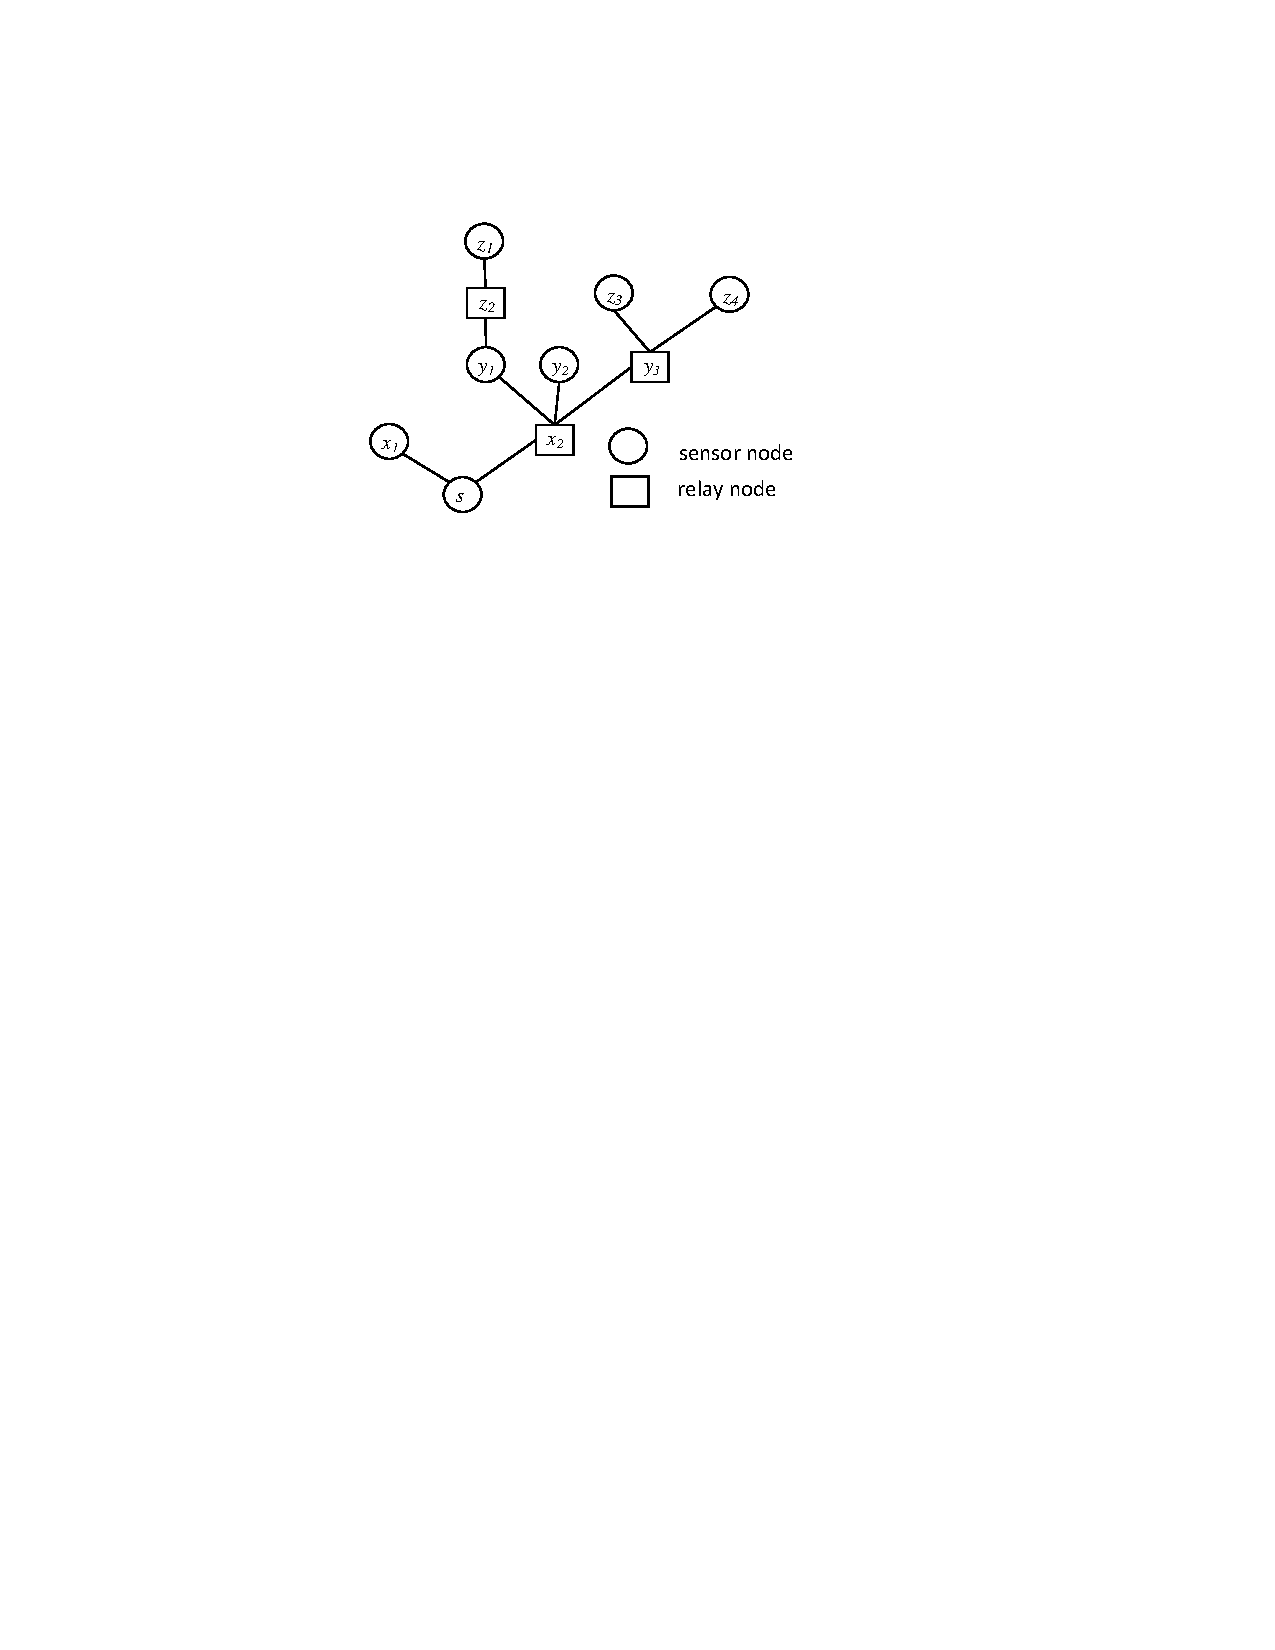
\includegraphics[width=1.7 in, height=0.8 in]{Ch4f1.pdf}
 \caption{ A tree network}
\label{fig:es31}
\end{figure}
\end{columns}

\begin{example}
\normalfont
In figure , consider node $x_2$. $n(V_{x_2})=8$ where $n_{sense}(V_{x_2})=5$ and $n_{relay}(V_{x_2})=3$. Assuming $n_{req}=5$ in an instance of the $\SRCONN$ problem then $n_{sense,min}(V_{x_2})=3=n_{req}-n_{sense}(\{s,x_1\})=5-2$. 
\end{example}
\end{frame}
%------------------------
\begin{frame}
\frametitle{$\SRCONN$ problem}
\begin{figure}
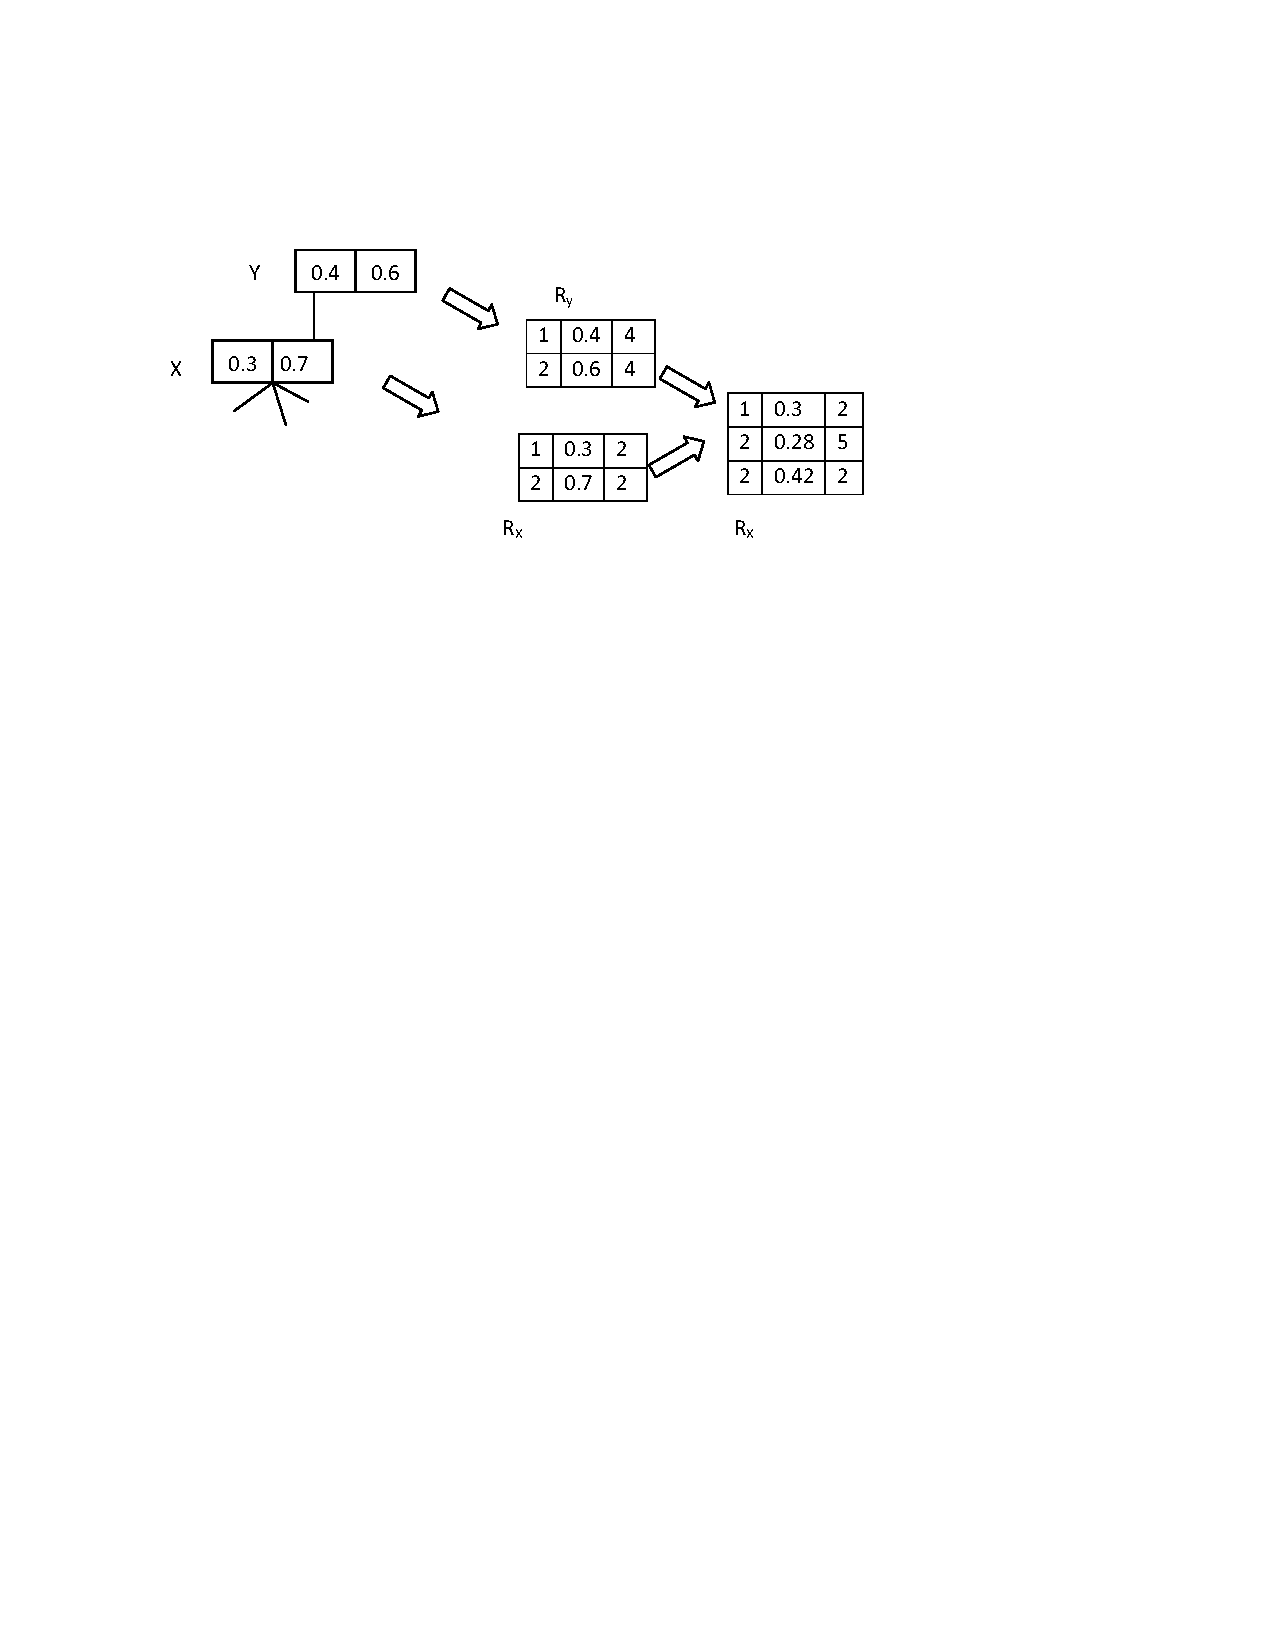
\includegraphics[scale=1]{Tree.pdf}
\caption{Table merge in Tree networks and $n_{req}=5$}
\end{figure}
\end{frame}

\begin{frame}
\frametitle{Pseudo-code for function Conn}
\vspace{-1.7em}
   % --------------- Function E2P ---------------
    \begin{figure}[htbp]
    % \begin{figure}[!ht]
    \small
\begin{center}
%\fbox{
    \begin{minipage}[t]{5 in}
    \renewcommand{\baselinestretch}{1}
    %
    {\bf Function $\fConn (G, T, \nReq)$}\\
	{\bf Input:}
	\begin{minipage}[t]{5in}
	the $SR$-$CONN$ problem where $G$ has a tree
	topology $T$ with no relay leaves
	\end{minipage}
	{\bf Output:}
	\begin{minipage}[t]{5in}
	$Conn(G, \nReq)$
	\end{minipage}
%
%\nwline
%	{\bf Notation:}
%	\begin{minipage}[t]{2.75in}
%	\end{minipage}
% --------------------
% initialization
   1.  \begin{minipage}[t]{5in}
       {\bf foreach} (node $x$ and a valid location index $i$) \\
         \iin{0.20} set $R_x(i, type(x) )= 1$ 
       \end{minipage}       
   2.  \begin{minipage}[t]{5in}
       {\bf while} ($T$ has at least 2 nodes) \\
       \{
       \end{minipage}
       \\
   3.  \iin{0.20} \begin{minipage}[t]{5 in}
   		  Let $y$ be a non-sink leaf of $T$, and $x= parent(y)$
		  \end{minipage}
		  \\
   4.  \iin{0.20} \begin{minipage}[t]{5 in}
   		  {\bf foreach} (key $(i,count) \in R_y$)
		       $R_y (i,count) \starEqual p_y(i)$
		  \end{minipage}
		  \\
   5.  \iin{0.20} \begin{minipage}[t]{5in}
   		  set $R'_x= \phi$
		  \end{minipage}
		  \\
   6.  \iin{0.20} \begin{minipage}[t]{5in}
   		  {\bf foreach} (pair of keys
		       		$\begin{array}[t]{l}
				 (i_x, count_x) \in R_x \mbox { and }
		   		 (i_y, count_y) \in R_y)
				 \end{array}
				$ \\ 
		  \{
		  \end{minipage}
		  \\
   7.  \iin{0.40} \begin{minipage}[t]{5 in}
   		  $count= \min (\nReq, count_x + count_y)$
		  \end{minipage}
		  \\
%   8.  \iin{0.40} \begin{minipage}[t]{5 in}
%   		  $count_{x,min}= \begin{array}[t]{l}
%		  		  type(x) + n_{y,min} + 
%		       	   	  \sum_{z \in \DCH(x)} n_{z,min}
%				  \end{array}$
%		  \end{minipage}
%		  \\
  8.  \iin{0.40} \begin{minipage}[t]{5 in}
   		  {\bf if} ($count < n_{sense,min}(\{x\}\cup V_y \cup_{z\in DCH(x)} V_z)$) {\bf continue} 
		  \end{minipage}
		  \\
   9.  \iin{0.35} \begin{minipage}[t]{5in}
   		  $R'_x (i_x,count) \plusEqual$ 
		  	$\begin{array}[t]{l}
			 R_y(i_y,count_y) \times 
			 R_x(i_x,count_x) \times 
			 E_G(x[i_x], y[i_y])
		  	 \end{array}$
		  \end{minipage}
		  \\
       \iin{0.40} \} \\
   10. \iin{0.20} \begin{minipage}[t]{5 in}
       		  set $R_x= R'_x$; remove $y$ from $T$
		   \end{minipage}
		   \\
       \iin{0.15} \} \\
   11. \begin{minipage}[t]{6 in}
       return $\sum_{s[i] \in \loc(s)} R_s(i,\nReq) * p_s(i)$
       \end{minipage}
       \\
    \end{minipage}	
%}
\end{center}
    \normalsize
    %
    \caption{Pseudo-code for function $\fConn$}
    \label{alg:Conn}
\vspace*{-0.1in}
    \end{figure}

\end{frame}
%-----------------------------------------
\begin{frame}
\frametitle{Running time}
Let $n$ be the number of nodes in $G$, and $\ell_{max}$ be the maximum
number of locations in the locality set of any node.

% ----------
\begin{theorem}
\normalfont
    Function $\fConn$ solves the $\SRCONN$ problem in
    $O(n \cdot n_{req}^2  \cdot \ell_{max}^2)$ time
\end{theorem}
{\bf Proof.}
We note the following.
\begin{itemize}
\item   Step 1: storing the tree $T$ require $O(n)$ time.

\item	Step 2: the main loop performs $n-1$ iterations.
	Each of Steps 3, 5, and 10 can be done in constant time.

\item	Step 4: this loop requires $O(\nReq \cdot \ell_{max})$ time.

\item	Step 6: this loop requires $O(n_{req}^2 \cdot \ell_{max}^2)$ iterations.
	Steps 7, 8, and 9 can be done in constant time.
\end{itemize}
Thus, the overall running time is $O(n \cdot n_{req}^2  \cdot \ell_{max}^2)$ time.

\begin{theorem}
\normalfont
    Function $\fConn$ solves the $\ARCONN$ problem in
    $O(n \cdot \ell_{max}^2)$ time

    % Overall: $O(n \cdot \ell_{max} + n \cdot \ell_{max}^2)$
\end{theorem}
\end{frame}
%-----------------------------------------


\section{$\ACONN$ problem}
%\subsection{Algorithm for $\ACONN$}
%\subsection{Simulation Results for $\ACONN$}
\begin{frame}
\frametitle{$\ACONN$ problem}
\begin{itemize}
\item Cliques for $\ACONN$
\item State types for $\ACONN$ problem
\item Algorithms for $\ACONN$ problem
\item simulation results for $\ACONN$ problem
\end{itemize}
\end{frame}
%-----------------------------------------
\begin{frame}
\frametitle{Cliques for $\ACONN$ problem}
\vspace{-1em}
\begin{itemize}
\item $K_{v_i,base}$ : the $k$-clique to which node $v_i$ is attached. For the 3-tree in the figure, $K_{v_i,base}$ is the triangle (3-clique) on nodes $\{v_j, v_k, v_l\}$.
\item $K_{v_i,1}, K_{v_i,2}, \ldots, K_{v_i,k}$ : all possible $k$-cliques involving node $v_i$ when this node becomes a $k$-leaf. For the 3-tree in the figure, we may set $K_{v_i,1}=$ the triangle $(v_i,v_j,v_k)$, $K_{v_i,2}=$ the triangle $(v_i,v_j,v_l)$, $K_{v_i,3}=$ the triangle $(v_i,v_k,v_l)$.
\end{itemize}
\vspace{-1em}
\begin{figure}[!htb]
\begin{minipage}{0.55\linewidth}
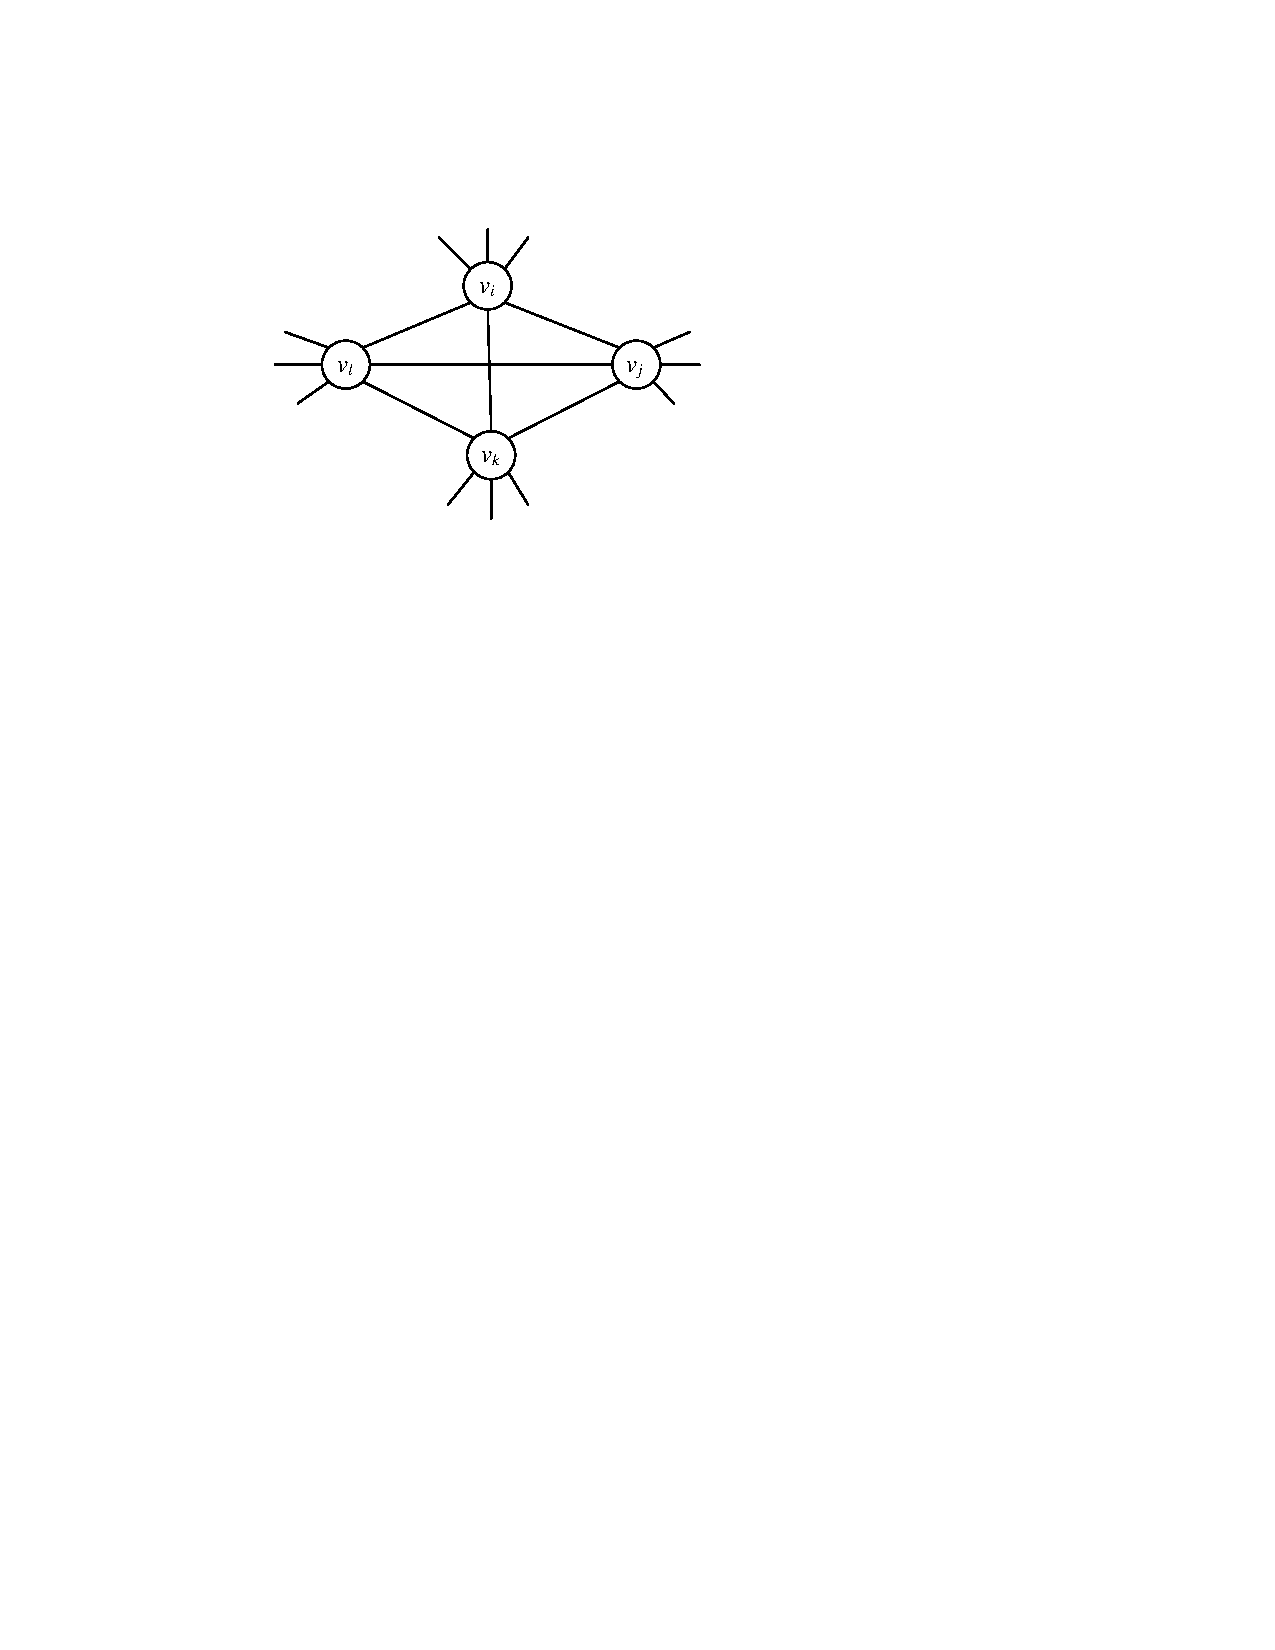
\includegraphics[width=2 in, height=0.8 in]{Ch3f1.pdf}
 \caption{ A fragment of a $3$-tree
 \label{fig:f3t}
}
\end{minipage}
\end{figure}
\end{frame}
%-----------------------------------------





%-----------------------------------------
\begin{frame}
\frametitle{State types for $\ACONN$ problem}
\vspace{-0.4 cm}
\centerline{
$A\mbox{-}type(S)=(V_1^{\loc(V_1)}, V_2^{\loc(V_2)}, \ldots, V_r^{\loc(V_r)})$}
\vspace{-0.4 cm}
\begin{figure}
\begin{minipage}{0.45\linewidth}
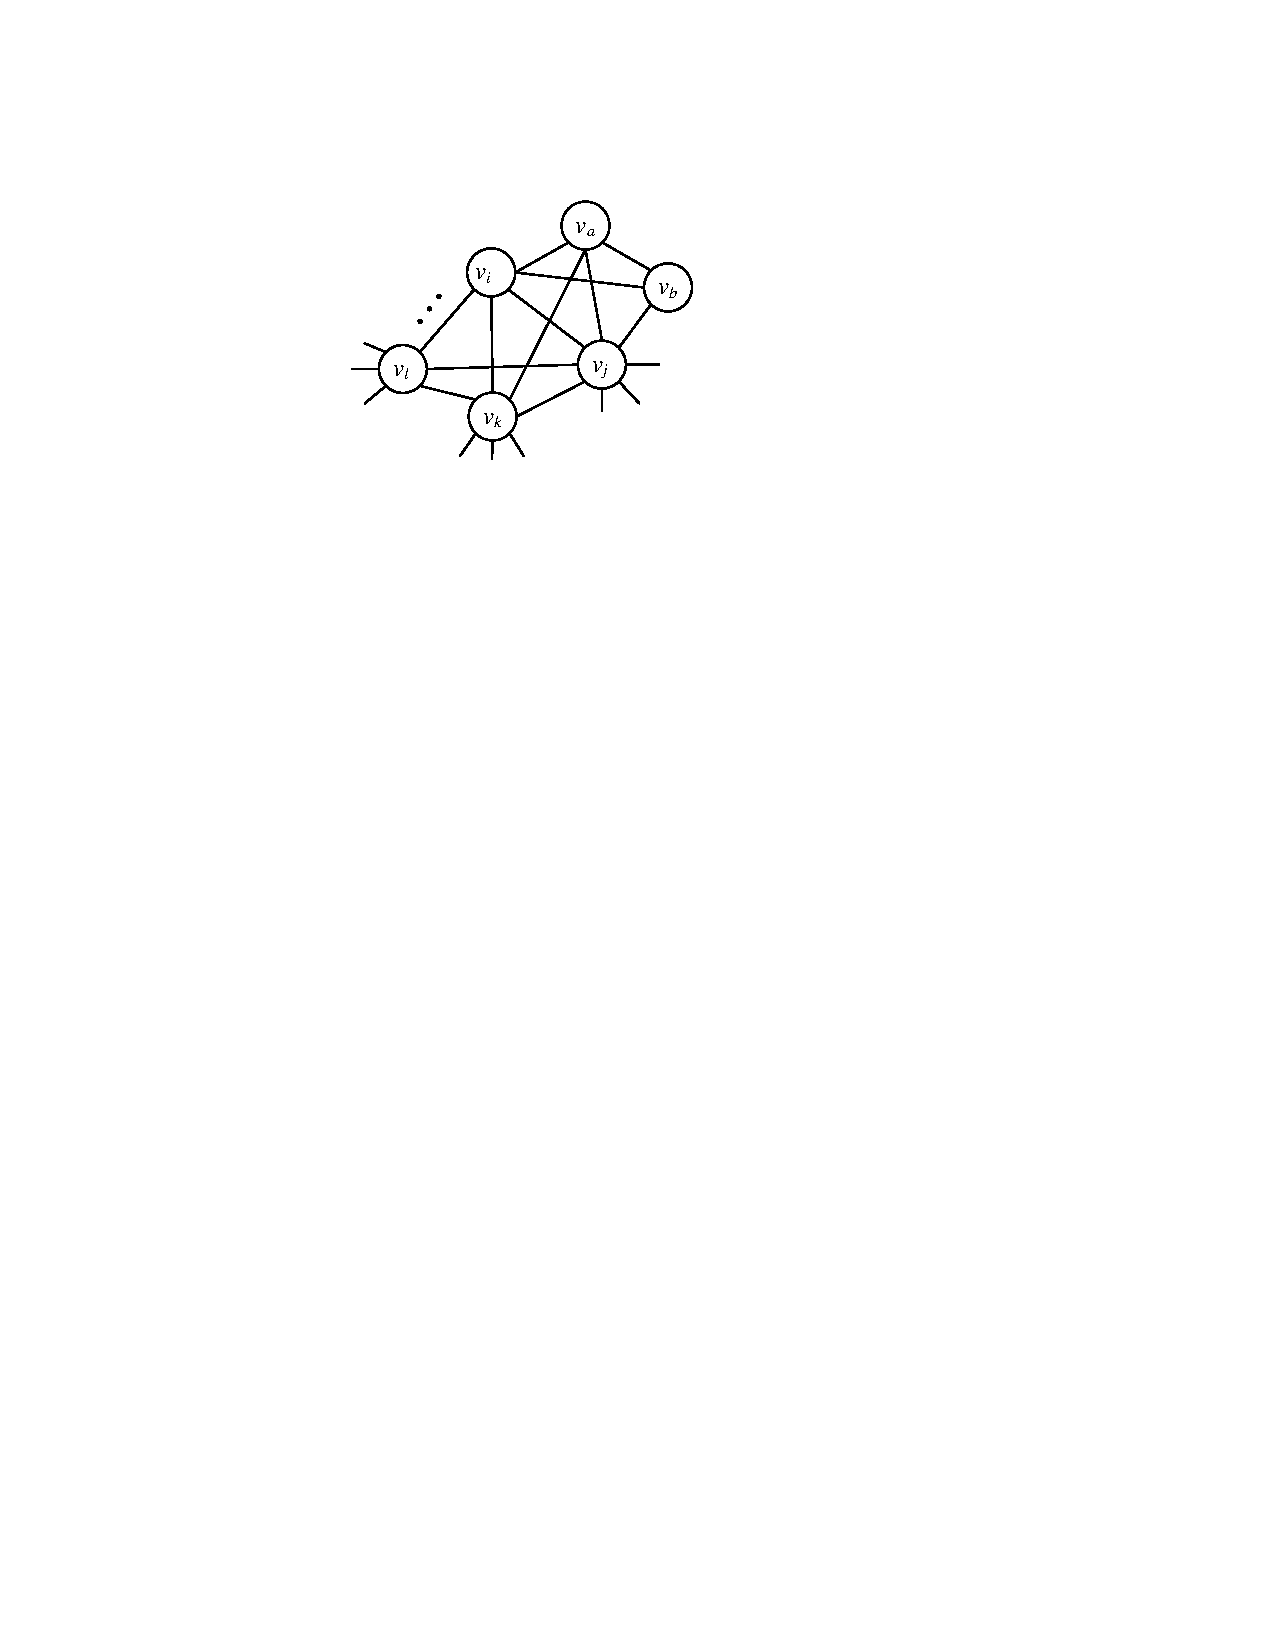
\includegraphics[width=1.6 in, height=0.7 in]{Ch3f2.pdf}
\vspace{-0.4 cm}
 \caption{ A 3-tree fragment}
 \label{fig:f32t1}
\end{minipage}
\begin{minipage}{0.5\linewidth}
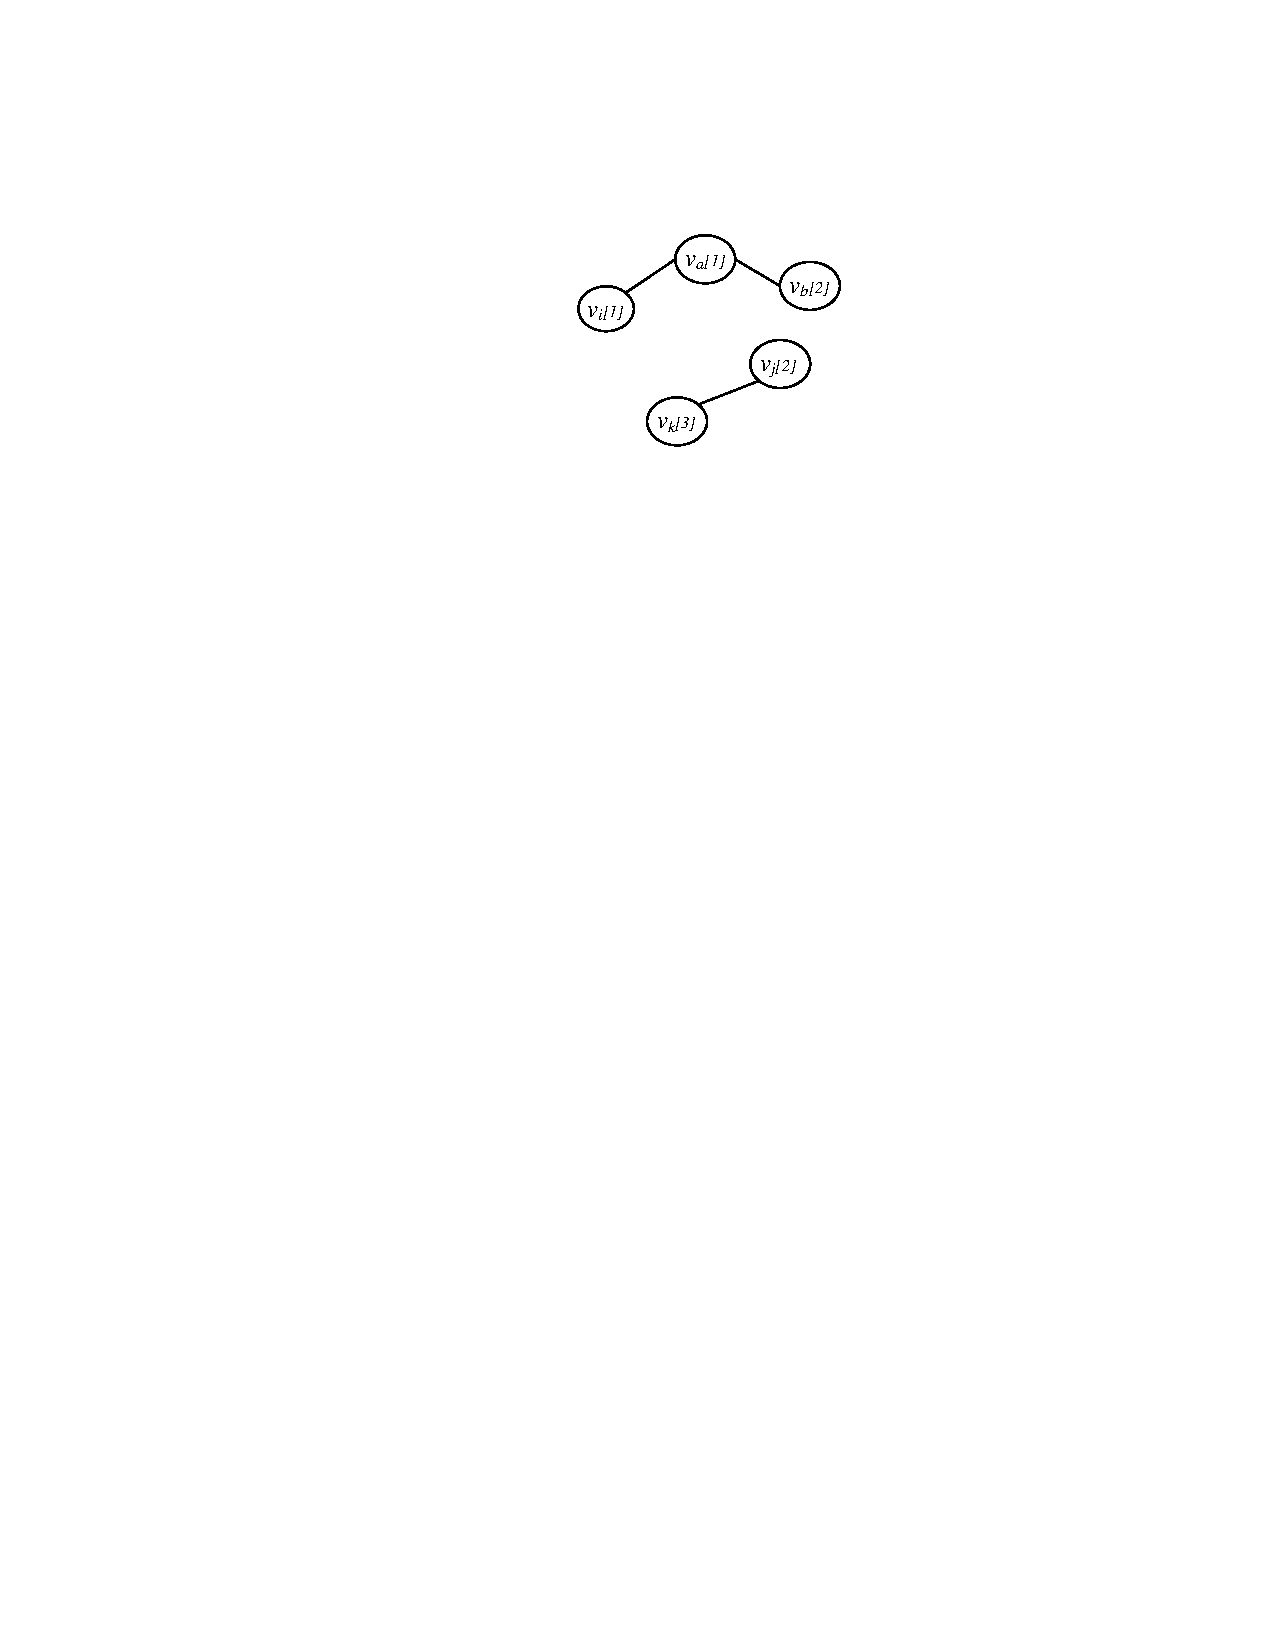
\includegraphics[width=1.6 in, height=0.7 in]{State.pdf}
\vspace{-0.4 cm}
 \caption{ A state of $\ACONN$ problem}
 \label{fig:f32t21}
\end{minipage}
\vspace{-0.4 cm}
\end{figure}
\vspace{-0.85em}
\begin{example}
\normalfont
\begin{itemize}
\item $G_{v_i,1}$ induced on  $\{v_a, v_b, v_i, v_j,v_k\}$.
\item Assuming $S=\{v_a[1], v_b[2], v_i[1], v_j[2], v_k[3]\}$ is a possible network state of $G_{v_i,1}$
\item Suppose that $S$ has 2 connected components : $\{v_a, v_b, v_i\}$ and $\{v_j, v_k\}$
\item Thus, $A\mbox{-}type(S)=(\{v_a,v_b,v_i\}^{(1,2,1)}, \{v_j,v_k\}^{(2,3)})$. 
\end{itemize} 
\end{example}
\end{frame}
%-----------------------------------------
%-----------------------------------------
\begin{frame}
\frametitle{A sample Table}
\vspace{-1.5em}
\begin{columns}
\column{0.5\textwidth}
A table $T_{v_i,\alpha}$, where $\alpha=base, 1, 2, \ldots, k$ is key-value mapping where
\begin{itemize}
\item a key is a network state type of the graph $G_{v_i,\alpha}$ 
\item each value is the probability.
\end{itemize}
\column{0.45\textwidth}
\begin{figure}[htbp]
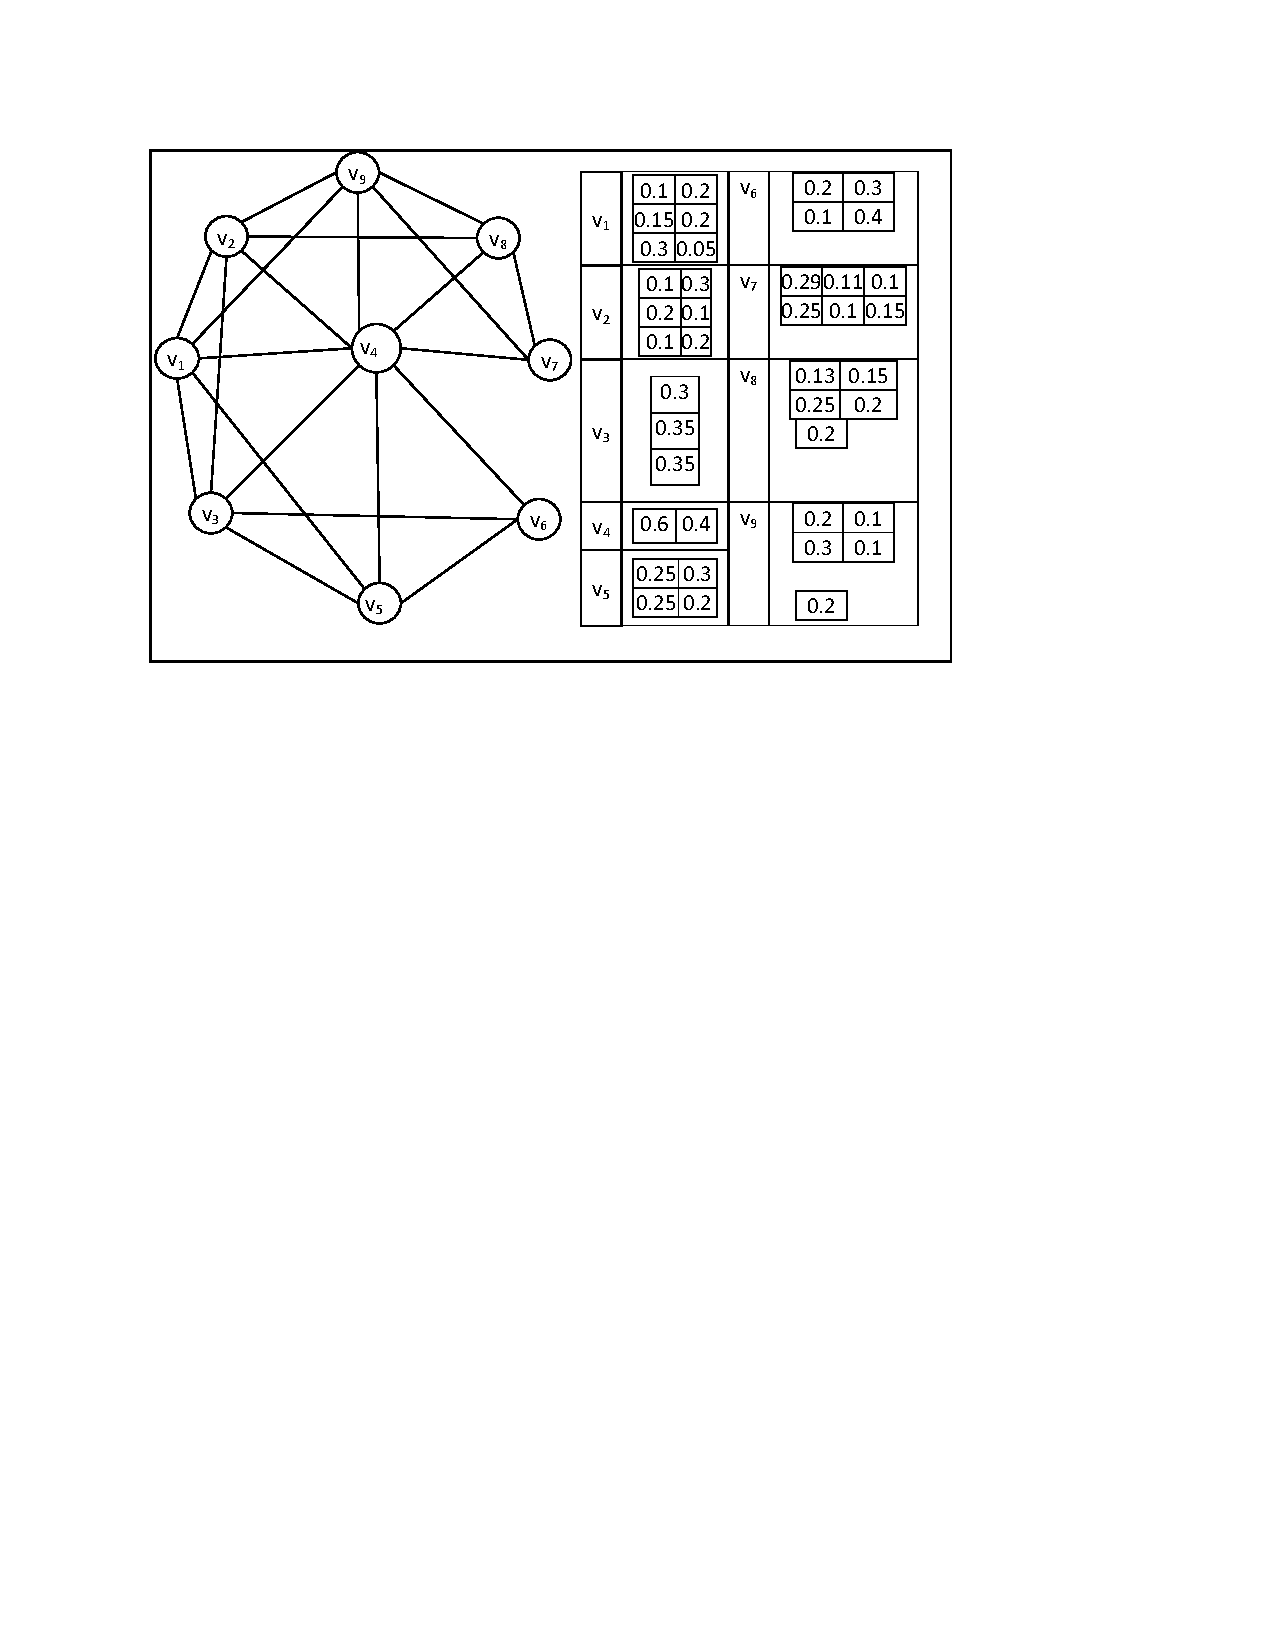
\includegraphics[width=2 in, height=1 in]{relay1.pdf}
 \caption{ A $3$-tree}
 \label{fig:3t}
\end{figure}
\end{columns}
\vspace*{-0.5 cm}
\begin{columns}
\column{0.65\linewidth}
\begin{example}
\begin{itemize}
\item The algorithm associates a table with each triangle.
\item Each triangle can be partitioned in 5 different ways
\item The number of possible keys that appear in the table of triangle $(v_1,v_2,v_3)$ is $5 \times 6 \times 6 \times 3=648$ Why? 
\end{itemize}
\end{example}
\column{0.35\linewidth}
\begin{figure}
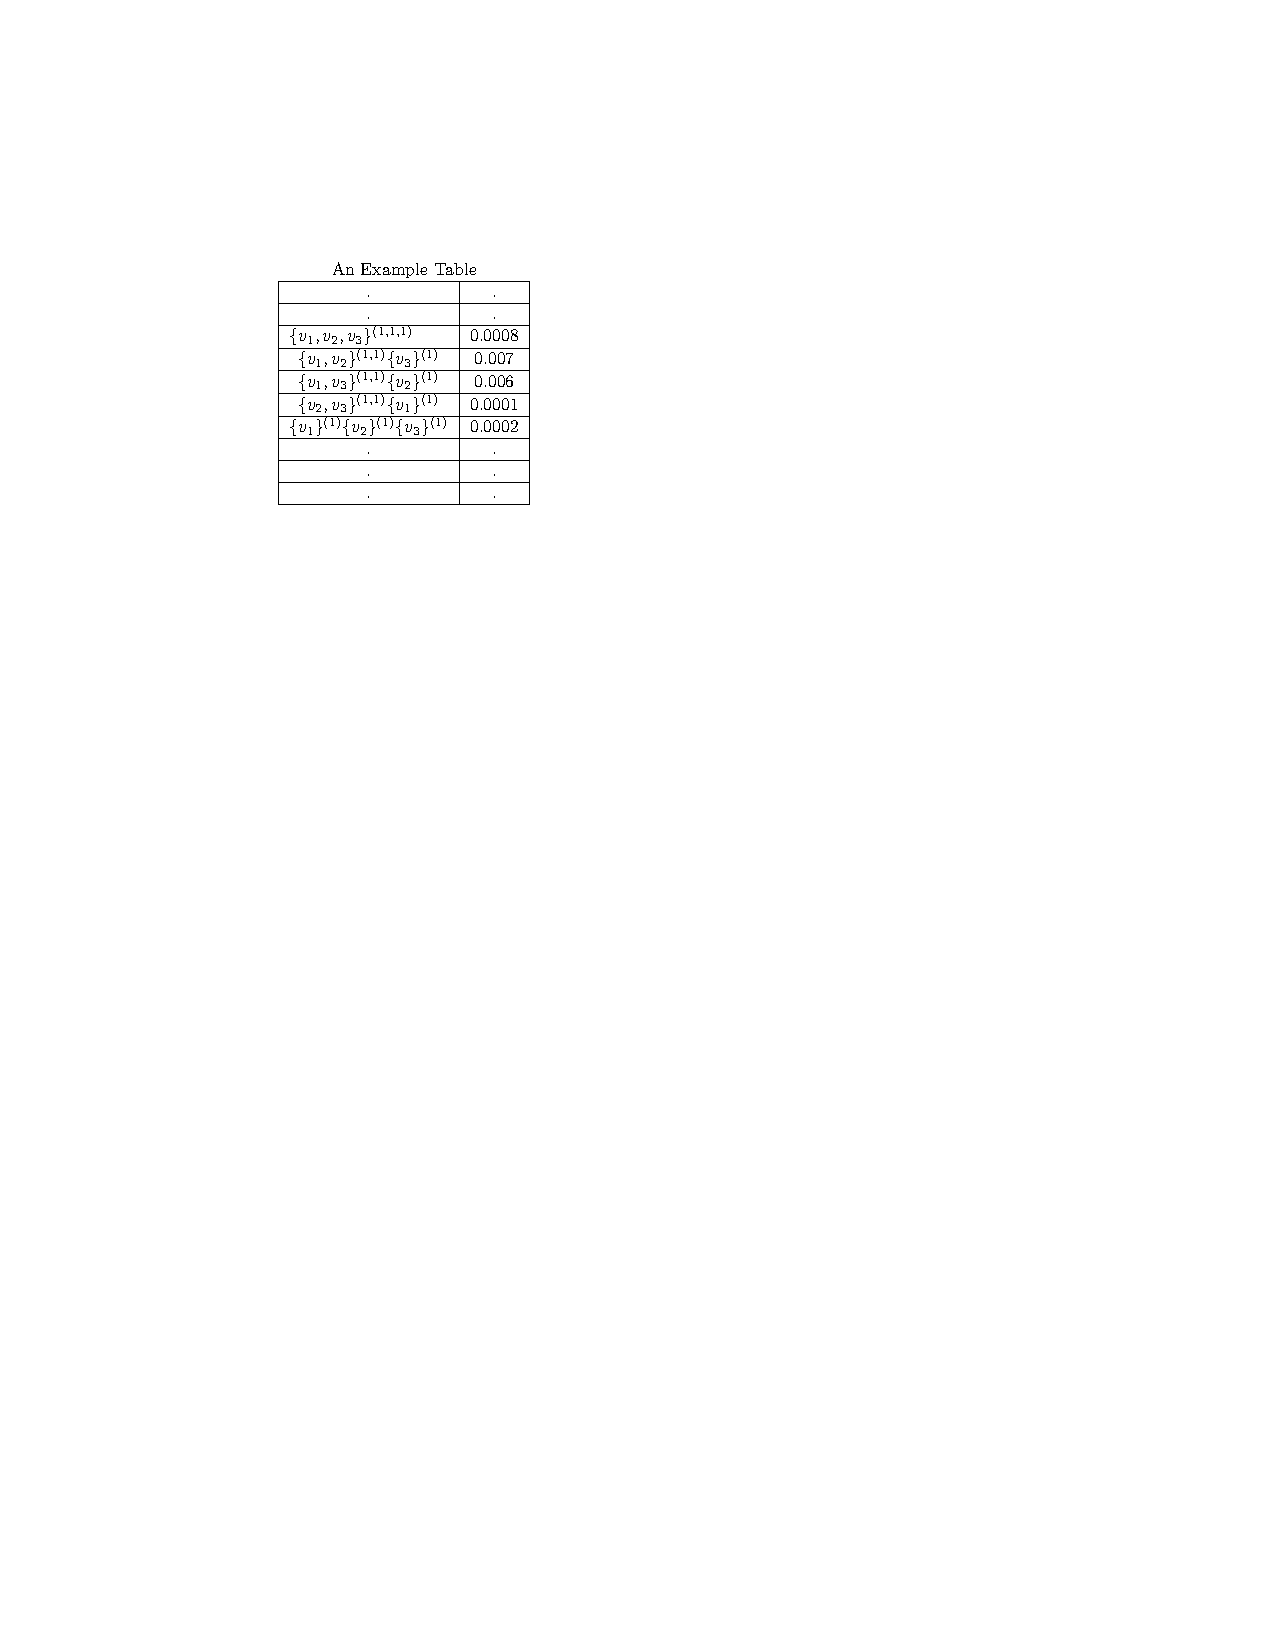
\includegraphics[scale=0.9]{Tab.pdf}
\end{figure}
\end{columns}
\end{frame}
%-----------------------------------------
\begin{frame}
\frametitle{Main Idea}
\begin{figure}
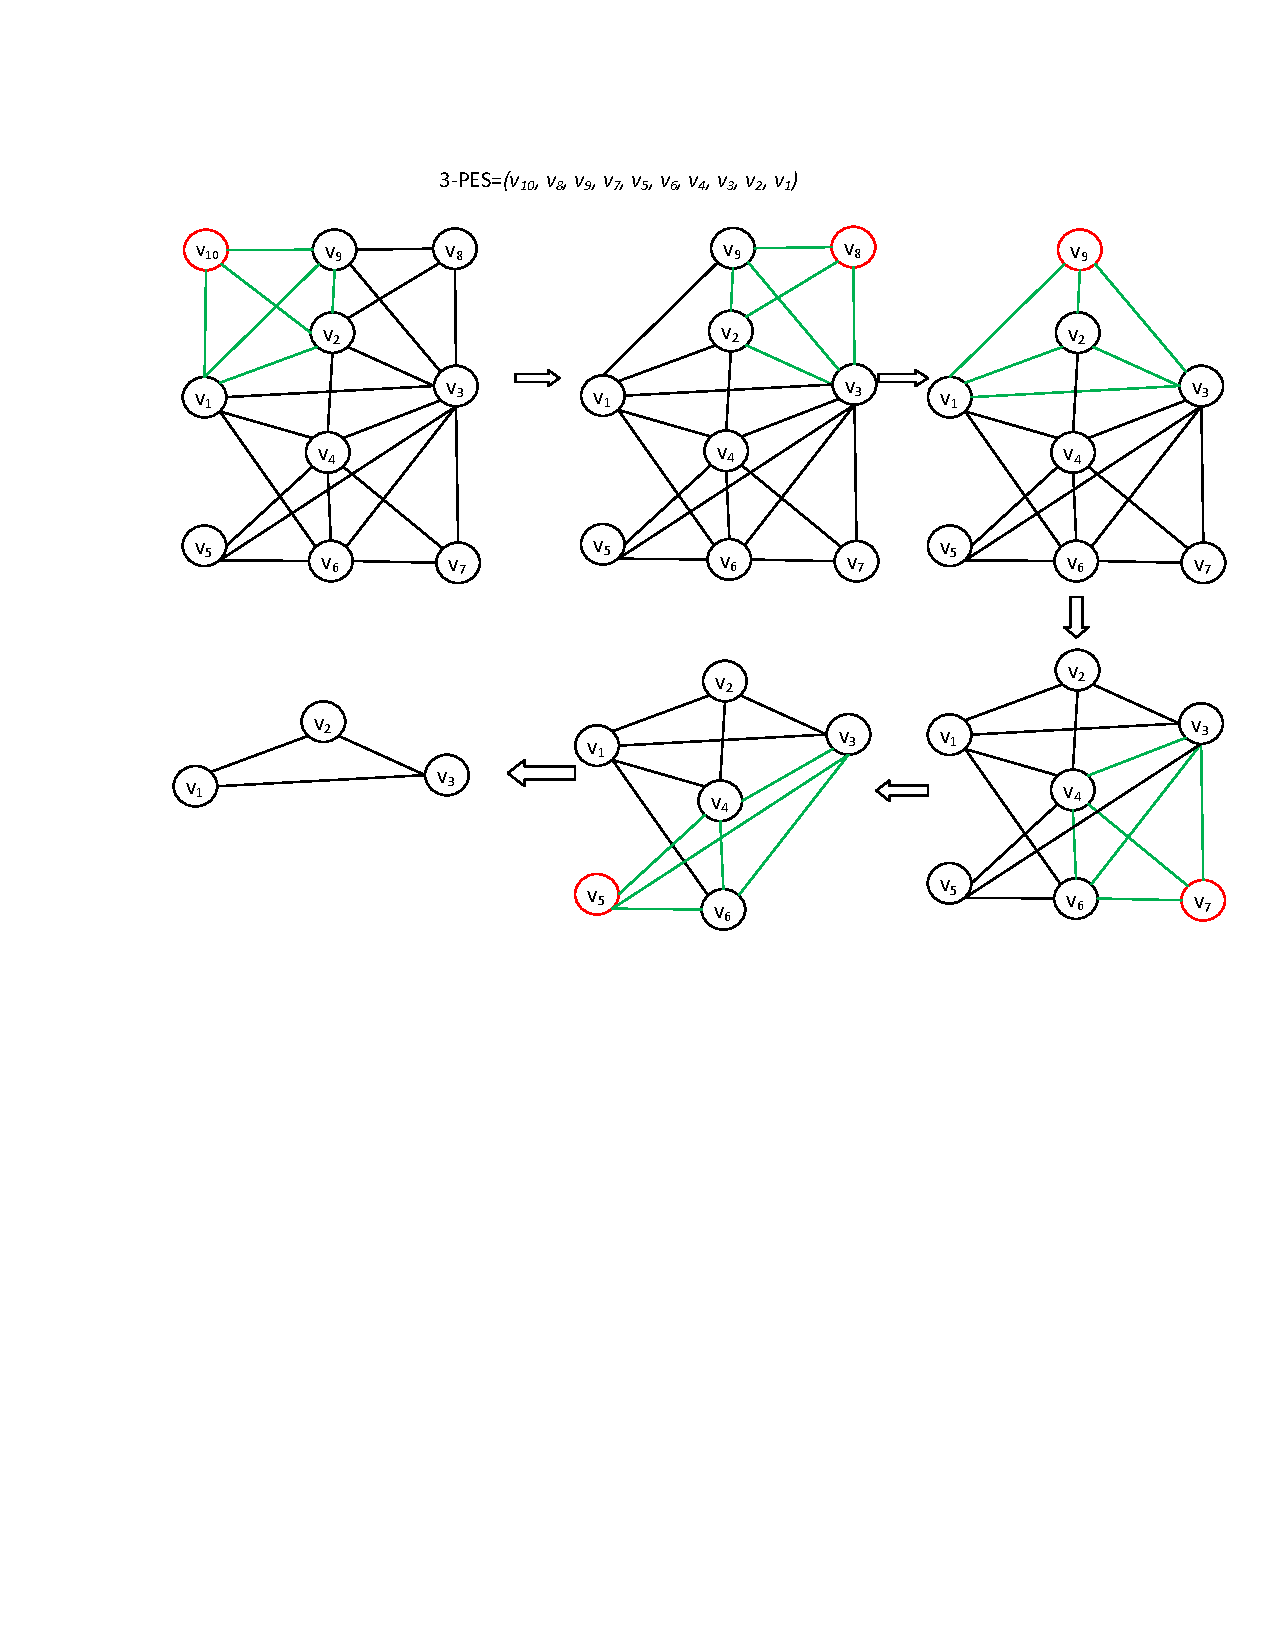
\includegraphics[height=2.4 in, width=4.5 in ]{Network1.pdf}
\caption{Mergeing Tables and Deleting nodes}
\end{figure}
\end{frame}
%------------------------------
\begin{frame}
\frametitle{Algorithm Organization}
The overall algorithm is organized around $3$ functions : 
\begin{itemize}
\item a top level main function
\begin{itemize}
\item process each node $v_i$ according to PES
\item finds all the tables associates with $v_i$ and merge them with the help of $t\_merge$
\item update the base table $T_{v_i,base}$ and removes node $v_i$
\end{itemize}
\item a middle level table merge function ( $t\_merge$), and
\begin{itemize}
\item merge tables with the help of $p\_merge$
\item updates the locality sets and probability
\end{itemize}
\item  a low level partition merge function ($p\_merge$)
\end{itemize}
\end{frame}
%-----------------------------------------
\begin{frame}

\frametitle{Table Merge and Partition merge}
\vspace{-1.1em}
\begin{figure}[htbp]
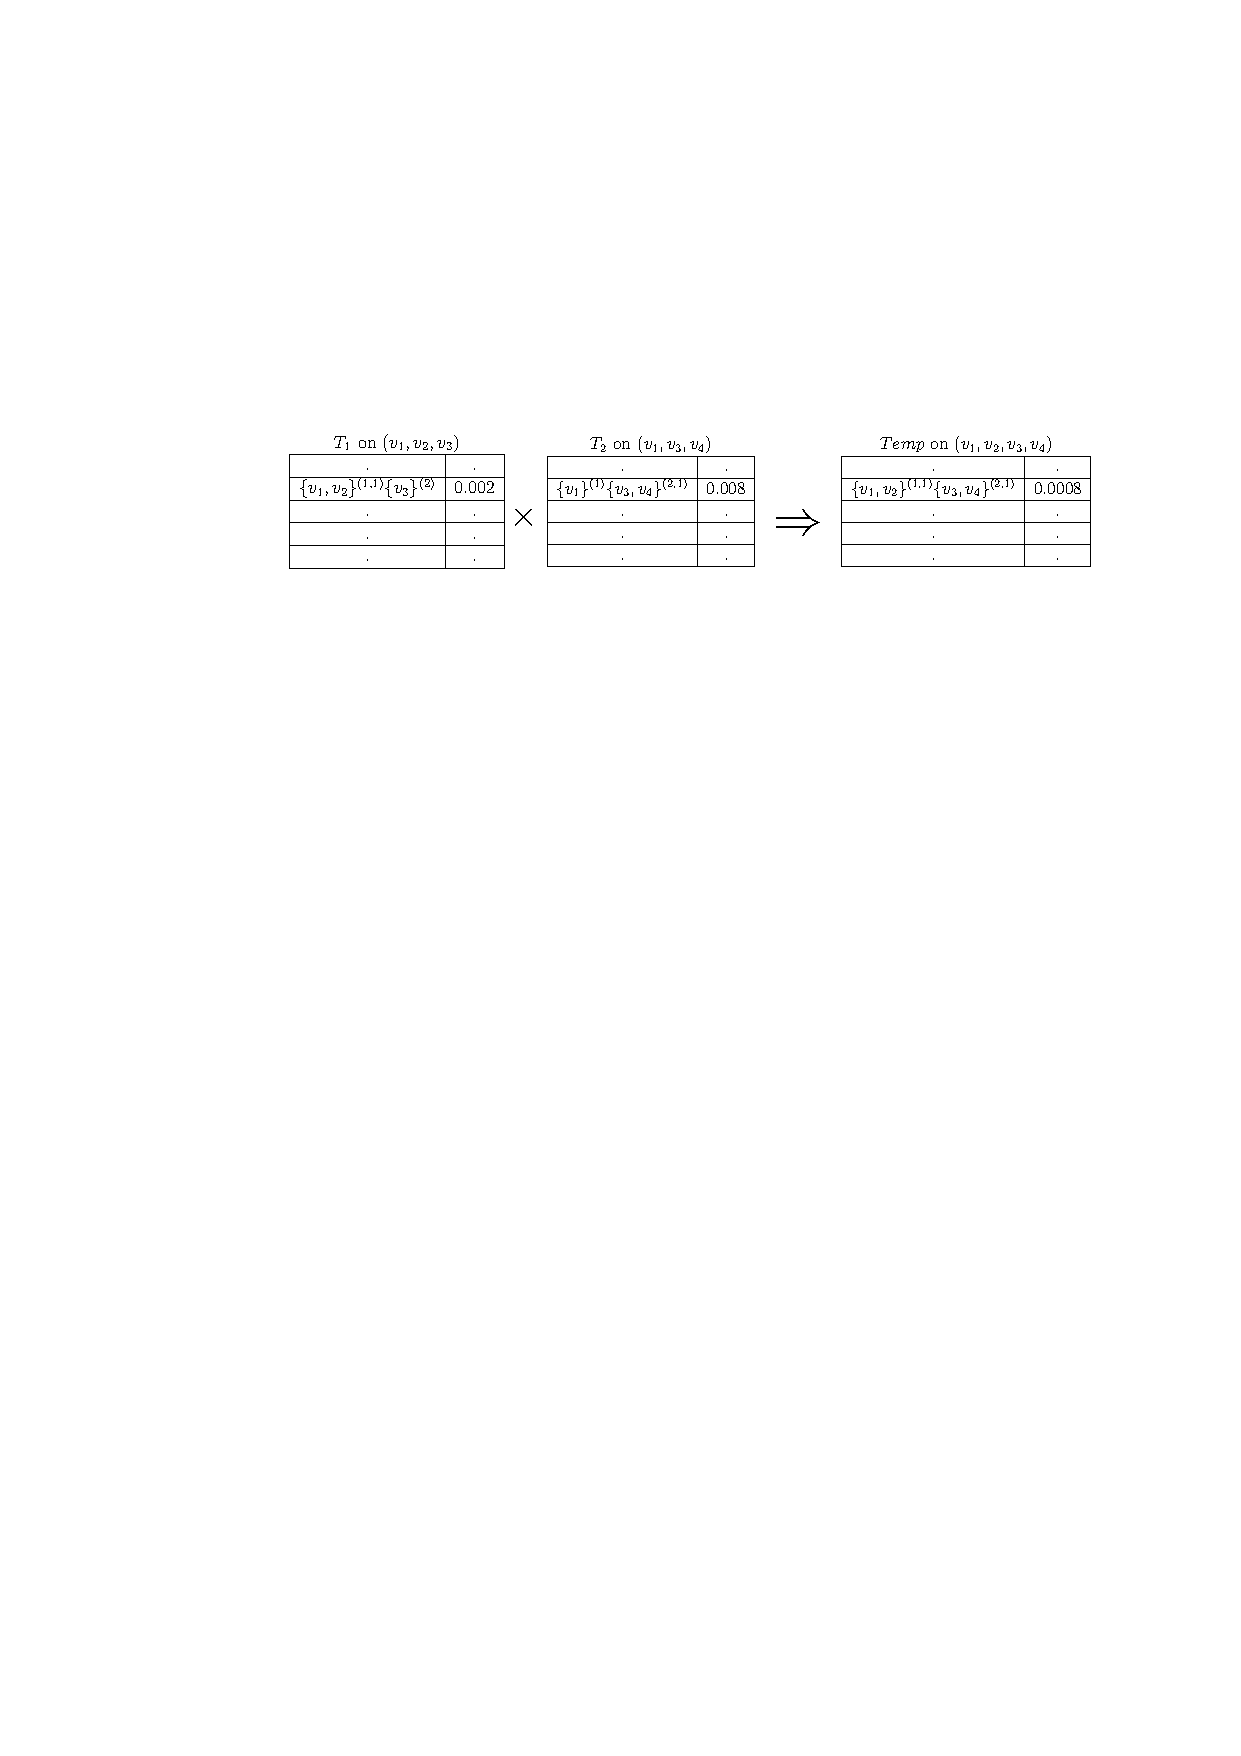
\includegraphics[width=3.8 in, height=1 in]{Table11.pdf}
\vspace*{-0.54 cm}
\caption{Operation in Table Merge }
\end{figure}

\begin{figure}[htbp]
\centering
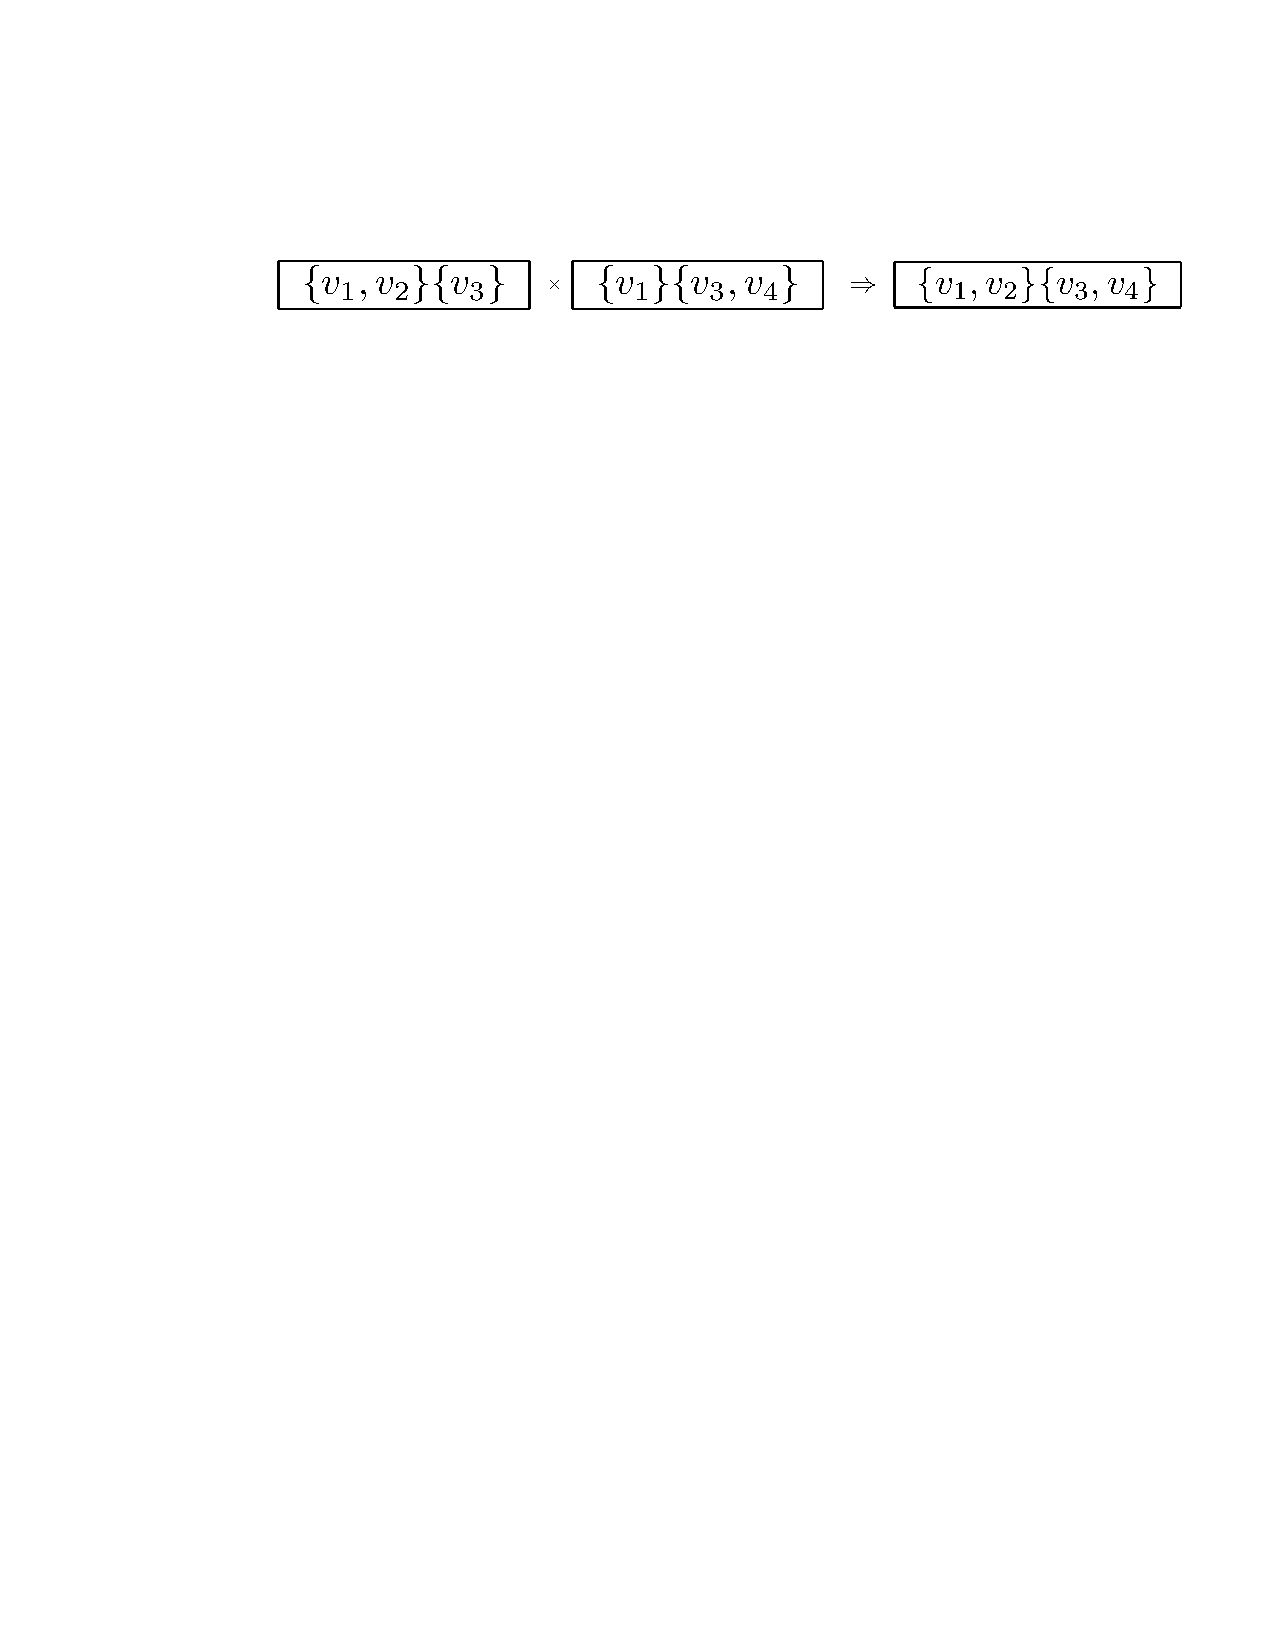
\includegraphics[width=3.8 in, height=0.2 in]{p_merge.pdf}
\vspace*{-0.354 cm}
\caption{Operation in Partition Merge}
\end{figure}

\begin{figure}[htbp]
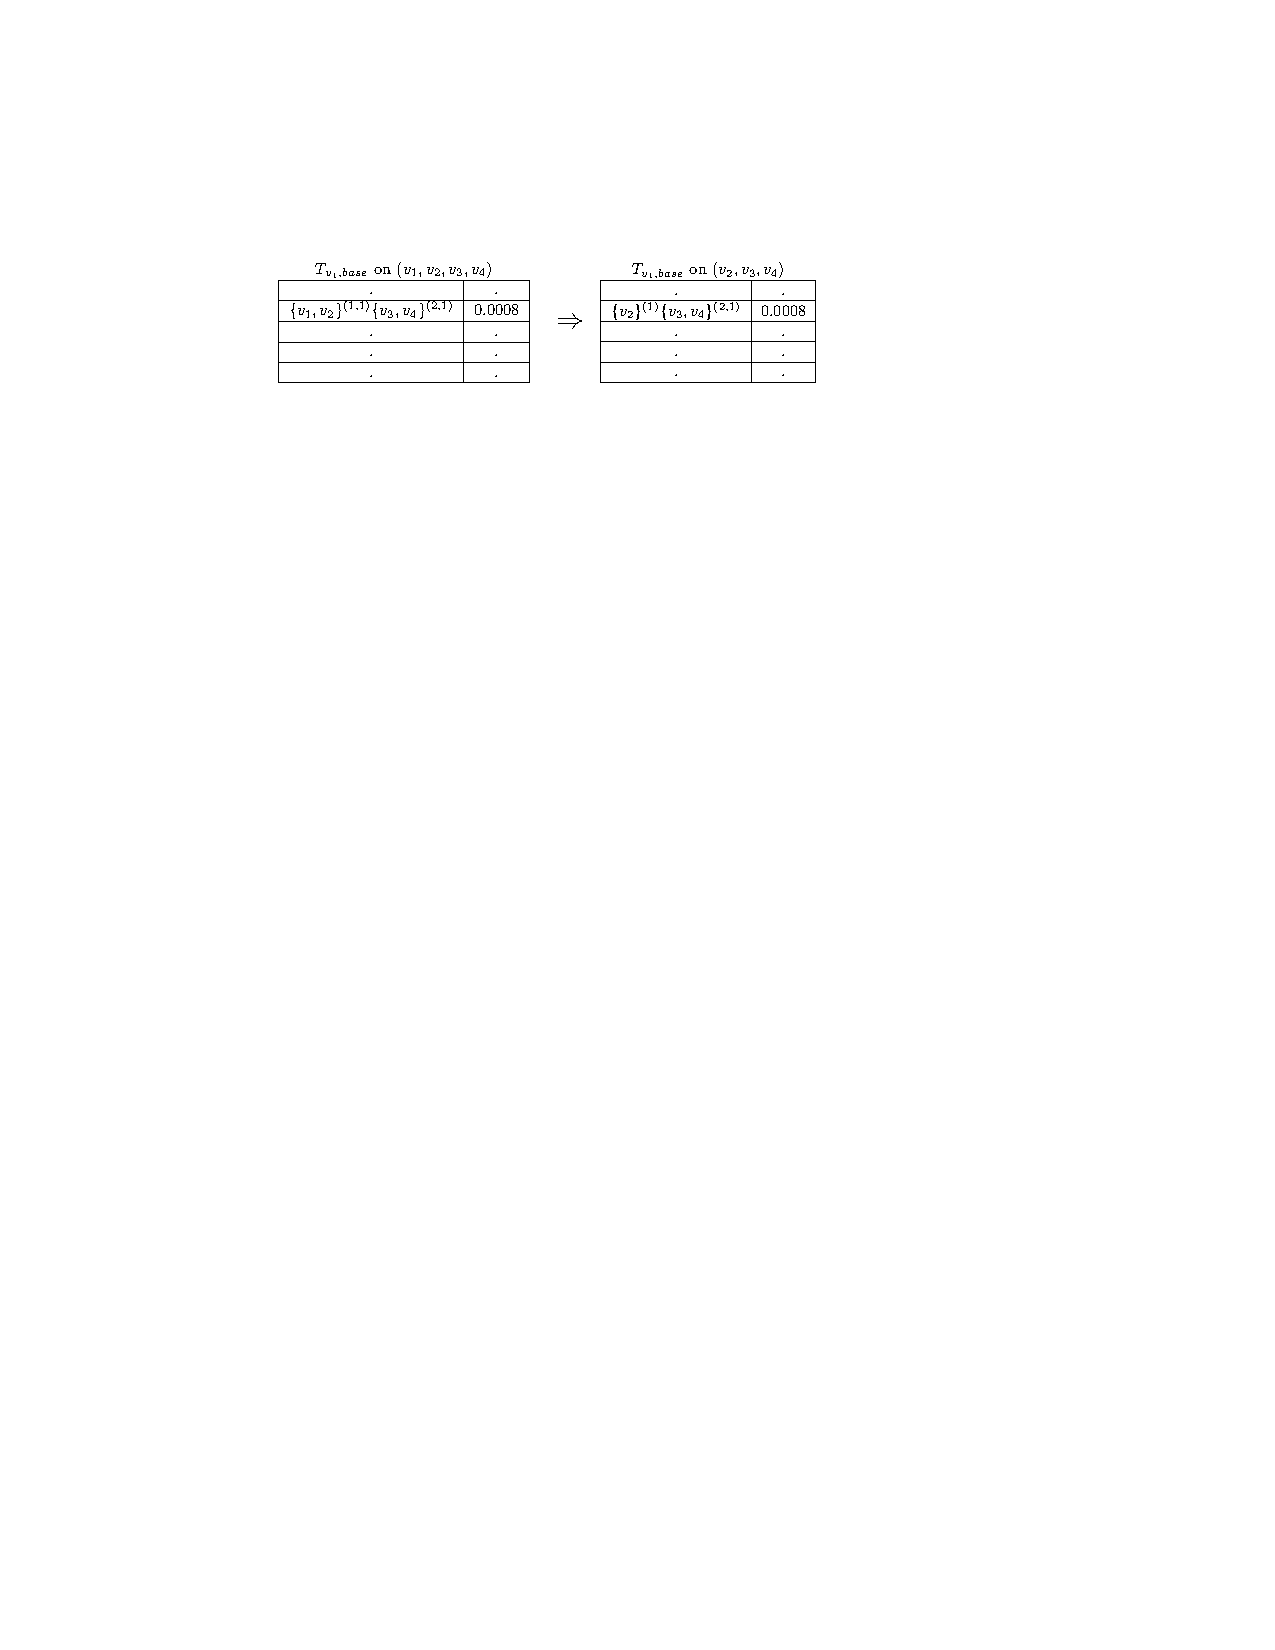
\includegraphics[width=3.8 in, height=1 in]{Table111.pdf}
\vspace*{-0.54 cm}
\caption{Operation in Main}
\end{figure}


\end{frame}

%-----------------------------------------
\begin{frame}
\frametitle{Function Main}
\vspace{-1.1em}
\begin{figure}[htbp]
\centering
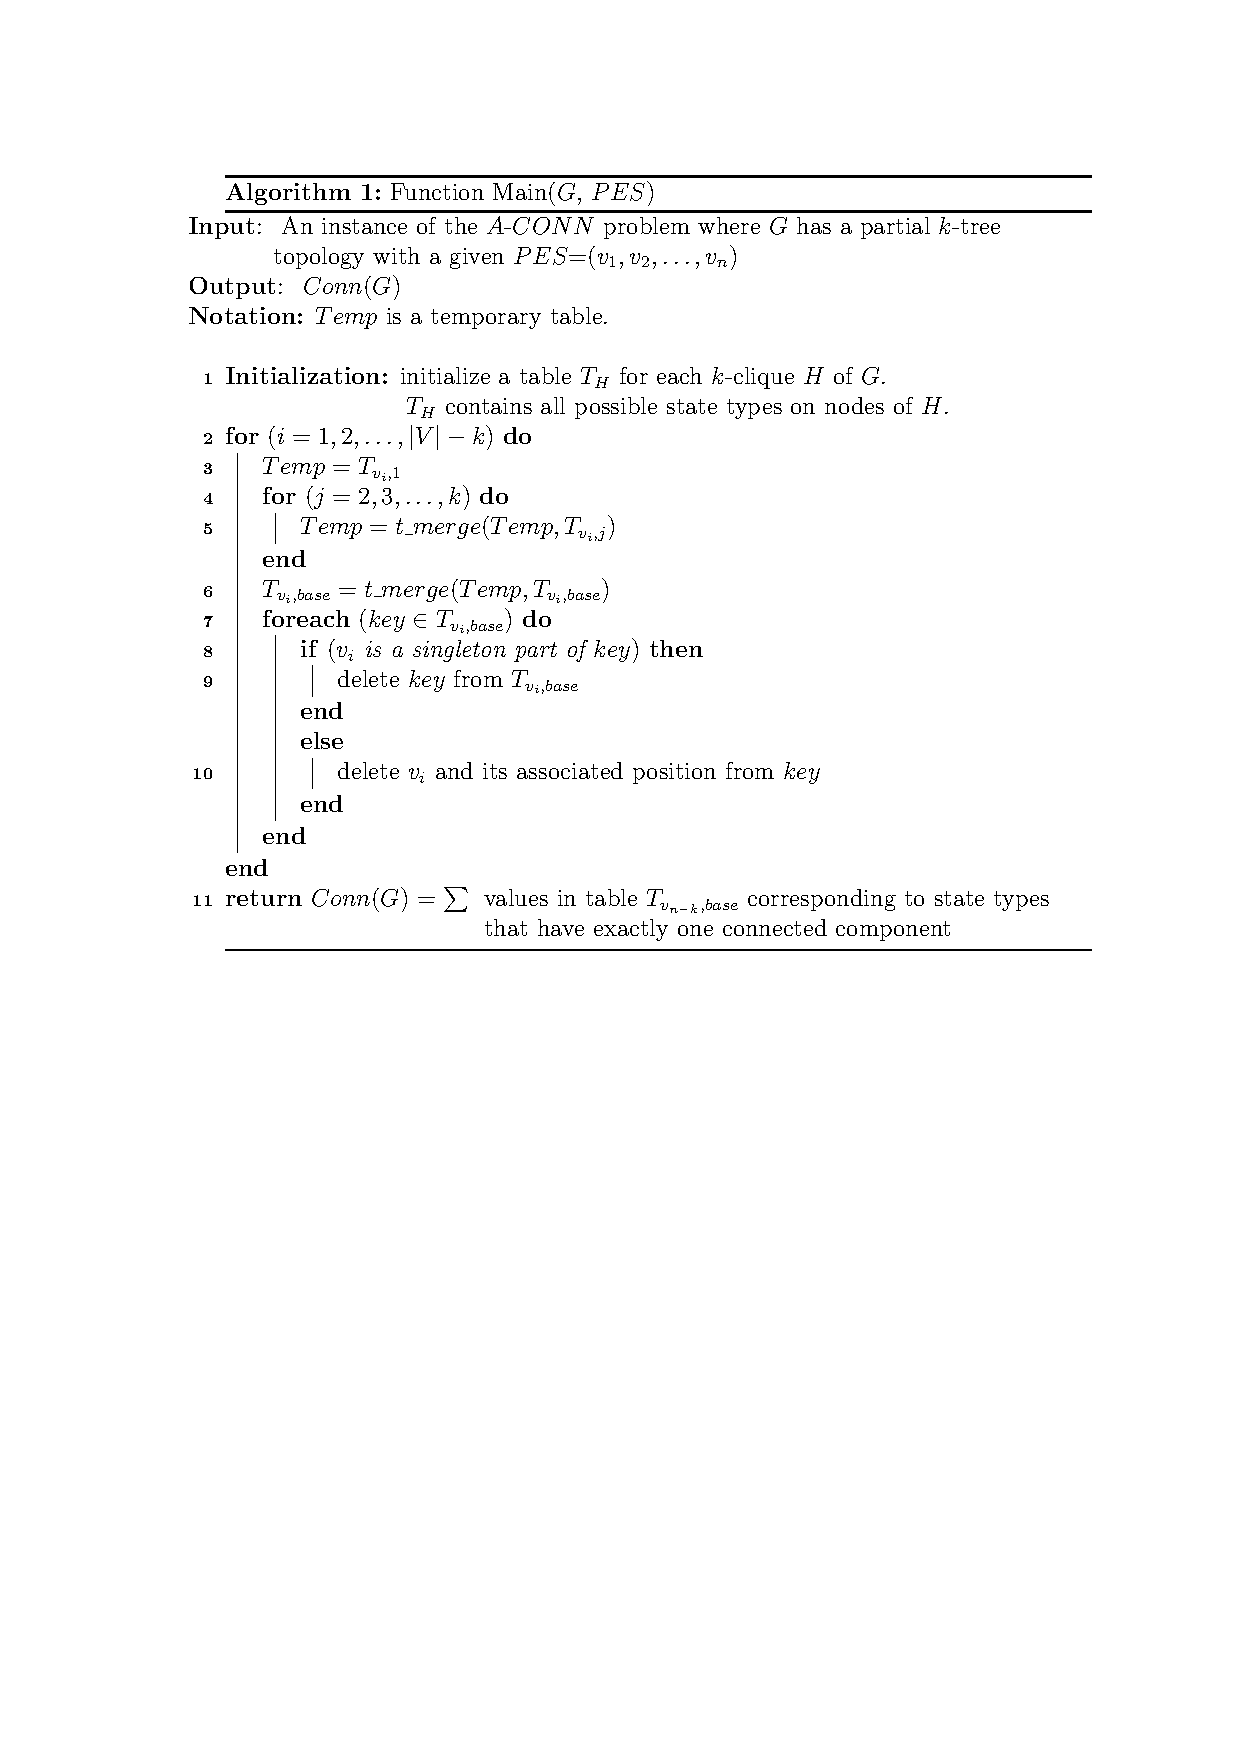
\includegraphics[width=3.8 in, height=3.2 in]{Fmain.pdf}
\end{figure}
\end{frame}

\begin{frame}
\frametitle{Running Time}
\begin{center}
\begin{theorem}\label{thm:runtym}
\normalfont
In the $\ACONN$ algorithm we have
\begin{enumerate}
\item The maximum length of any table is $\in O(B_k l_{max}^k)$.
\item The worst case running time is $O(n(B_k l_{max}^k)^2)$.
\end{enumerate}
\end{theorem}
\end{center}
\end{frame}
%-----------------------------------------
%\begin{frame}
%\frametitle{Function Table Merge}
%\vspace{-1.1em}
%\begin{figure}[htbp]
%\centering
%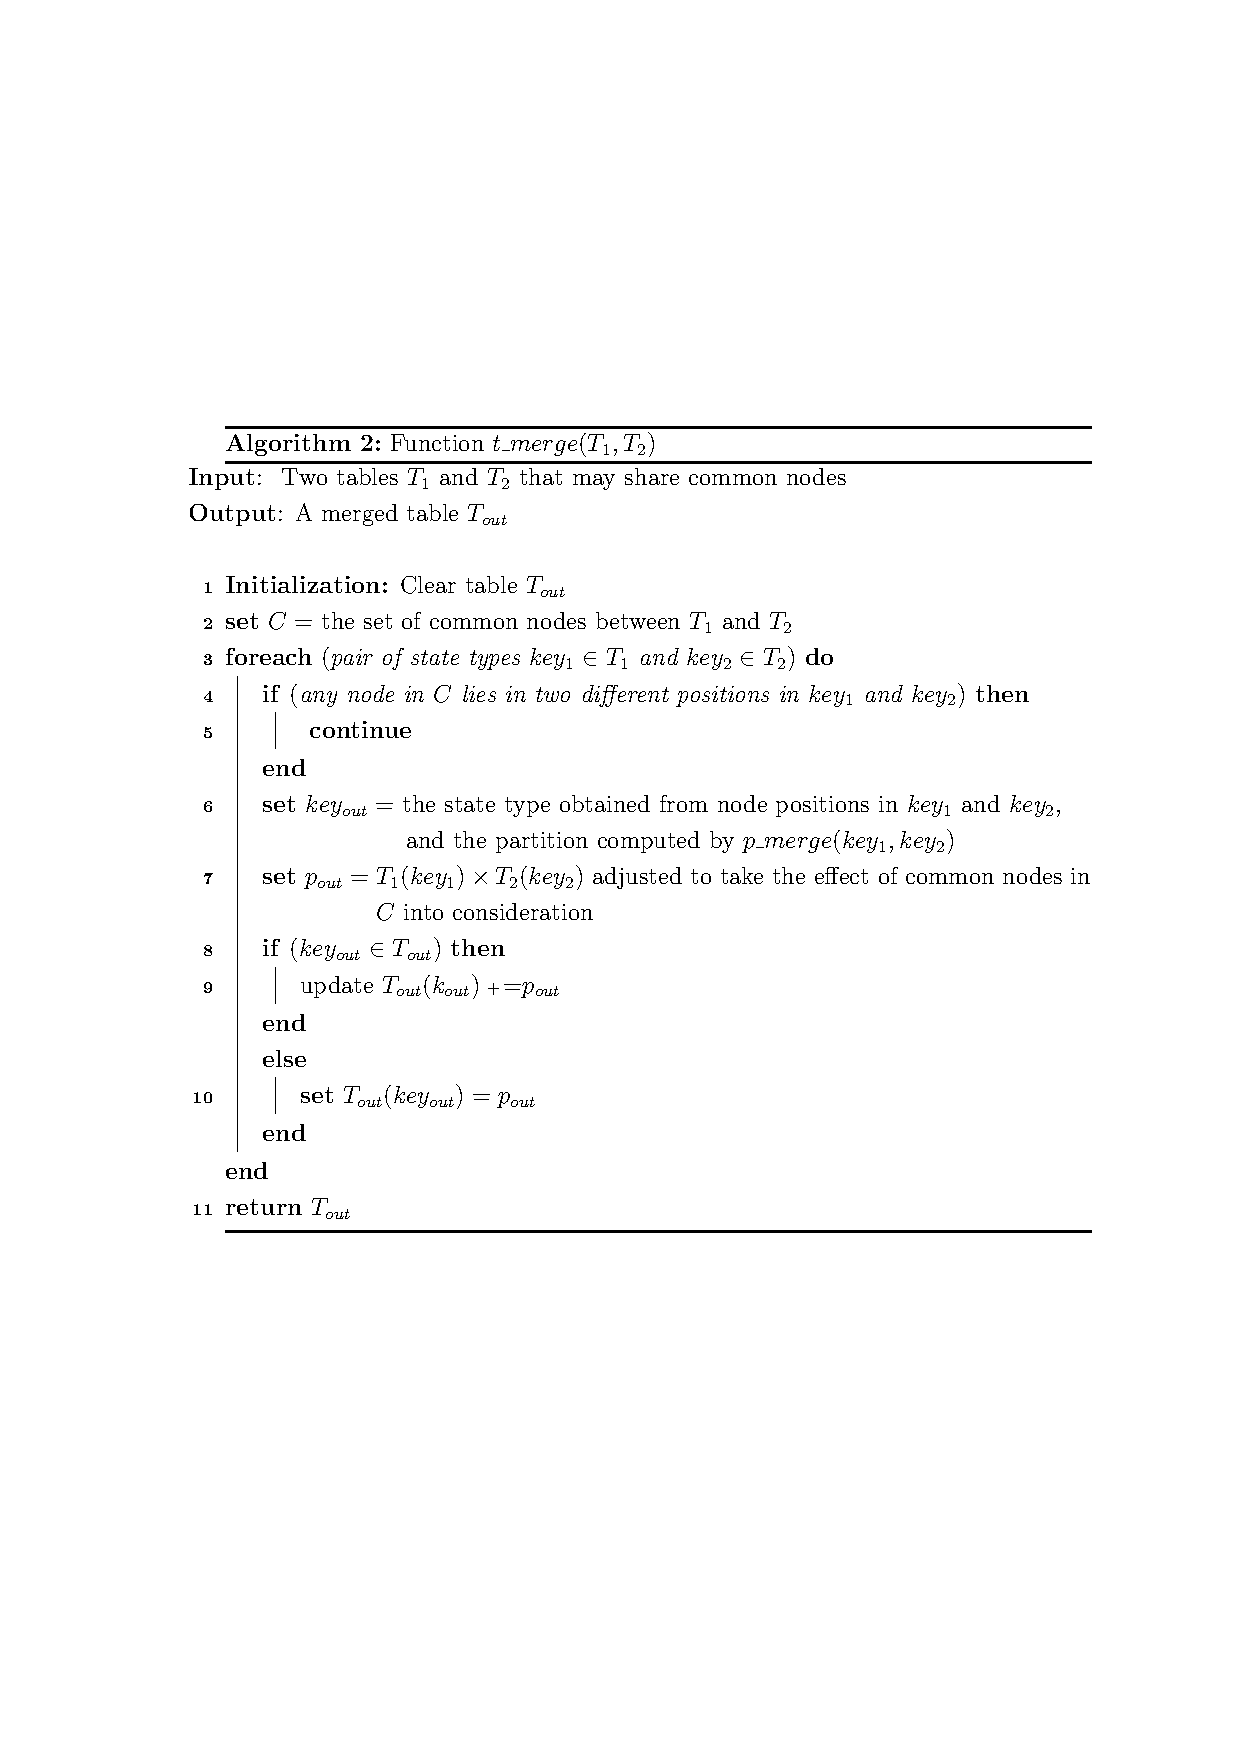
\includegraphics[width=3.8 in, height=3.2 in]{fmerge.pdf}
%\end{figure}
%\end{frame}
%
%%-----------
%%-----------------------------------------
%\begin{frame}
%\frametitle{Function Partition Merge}
%\vspace{-1em}
%
%\begin{figure}[htbp]
%\centering
%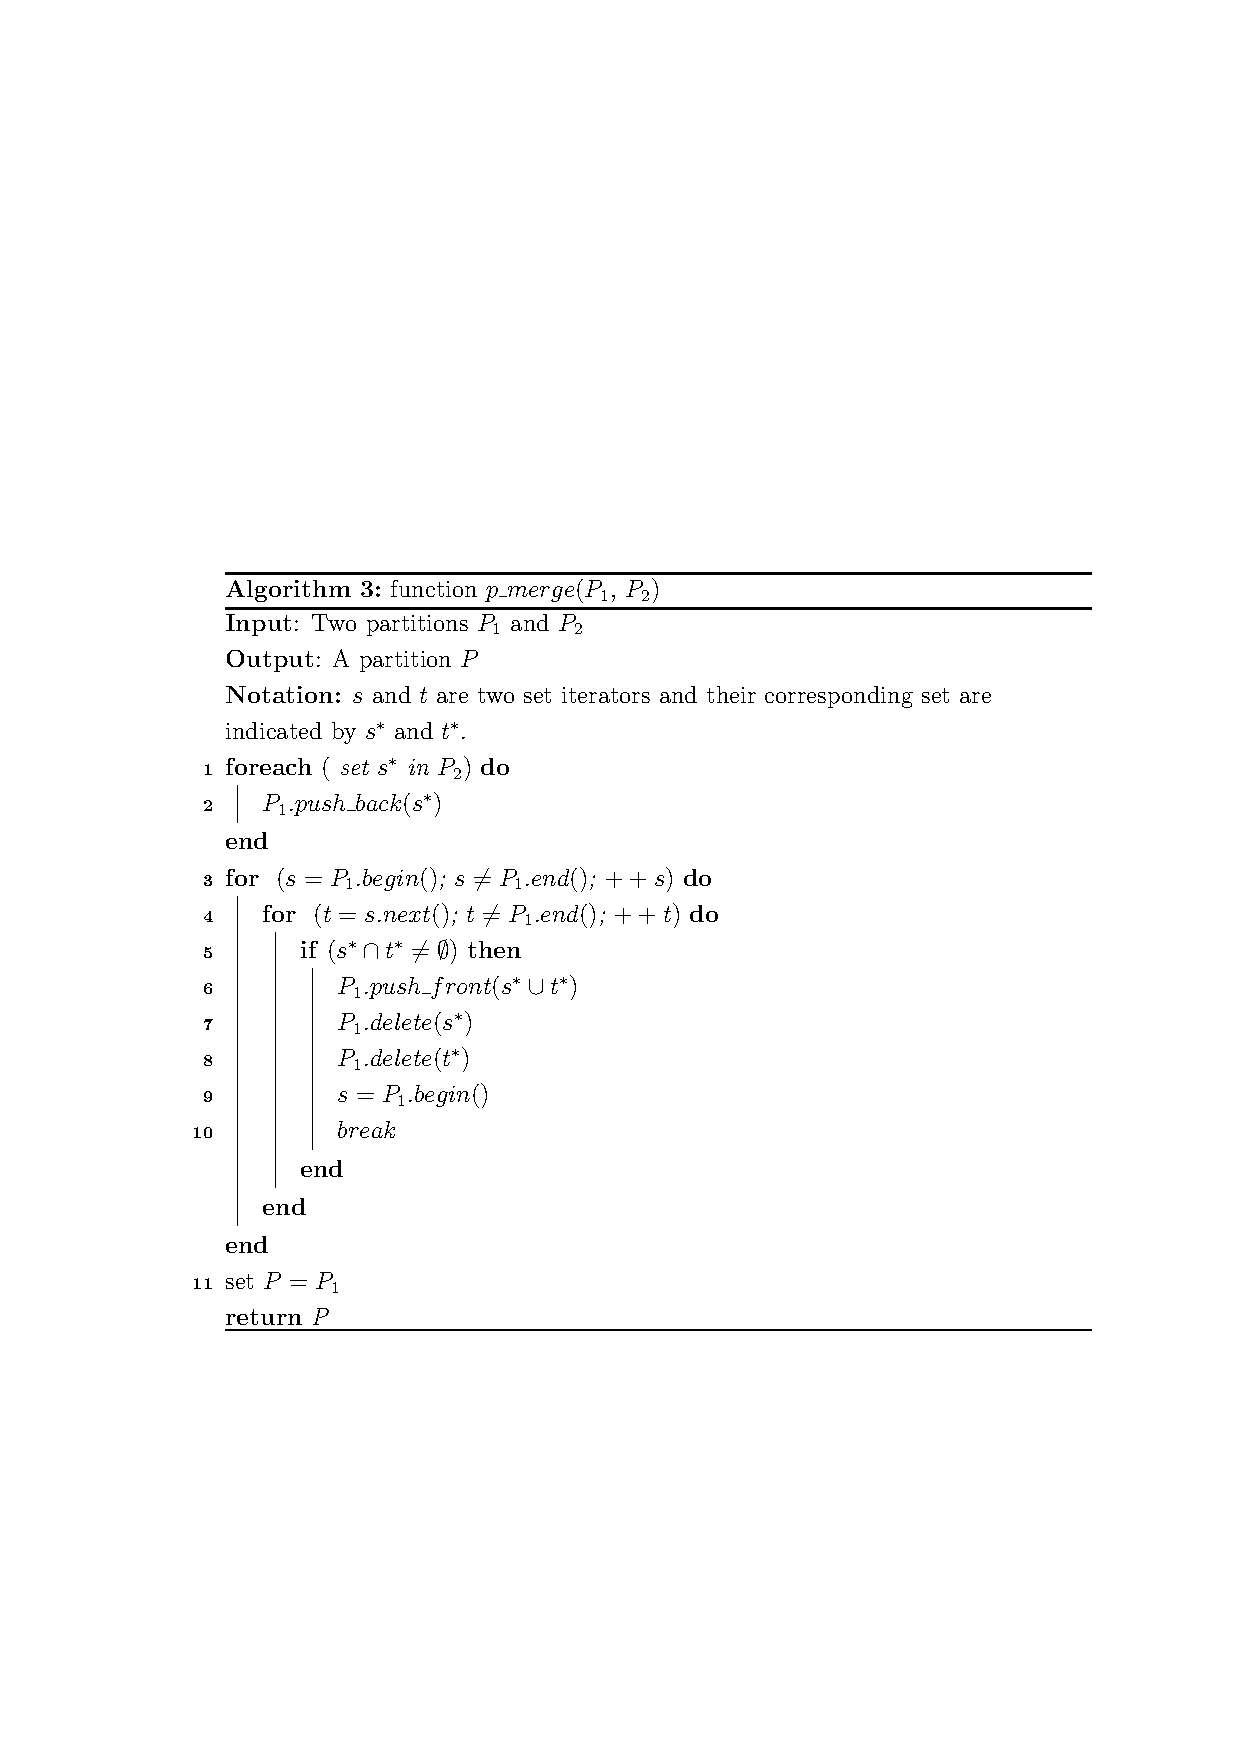
\includegraphics[width=3.8 in, height=2.7 in]{ftmerge.pdf}
%\end{figure}
%\end{frame}
%%-----------------------------------------

\begin{frame}
\frametitle{Simulation Results for $\ACONN$ problem}

\begin{itemize}
\item Test Networks
\item Running Time
\item Connectivity for different partial $k$-trees
\item Effect of subgraph selection method
\end{itemize}
\end{frame}
%-----------------------------------------
\begin{frame}
\frametitle{Test Networks}
\begin{figure}[htbp]
\centering
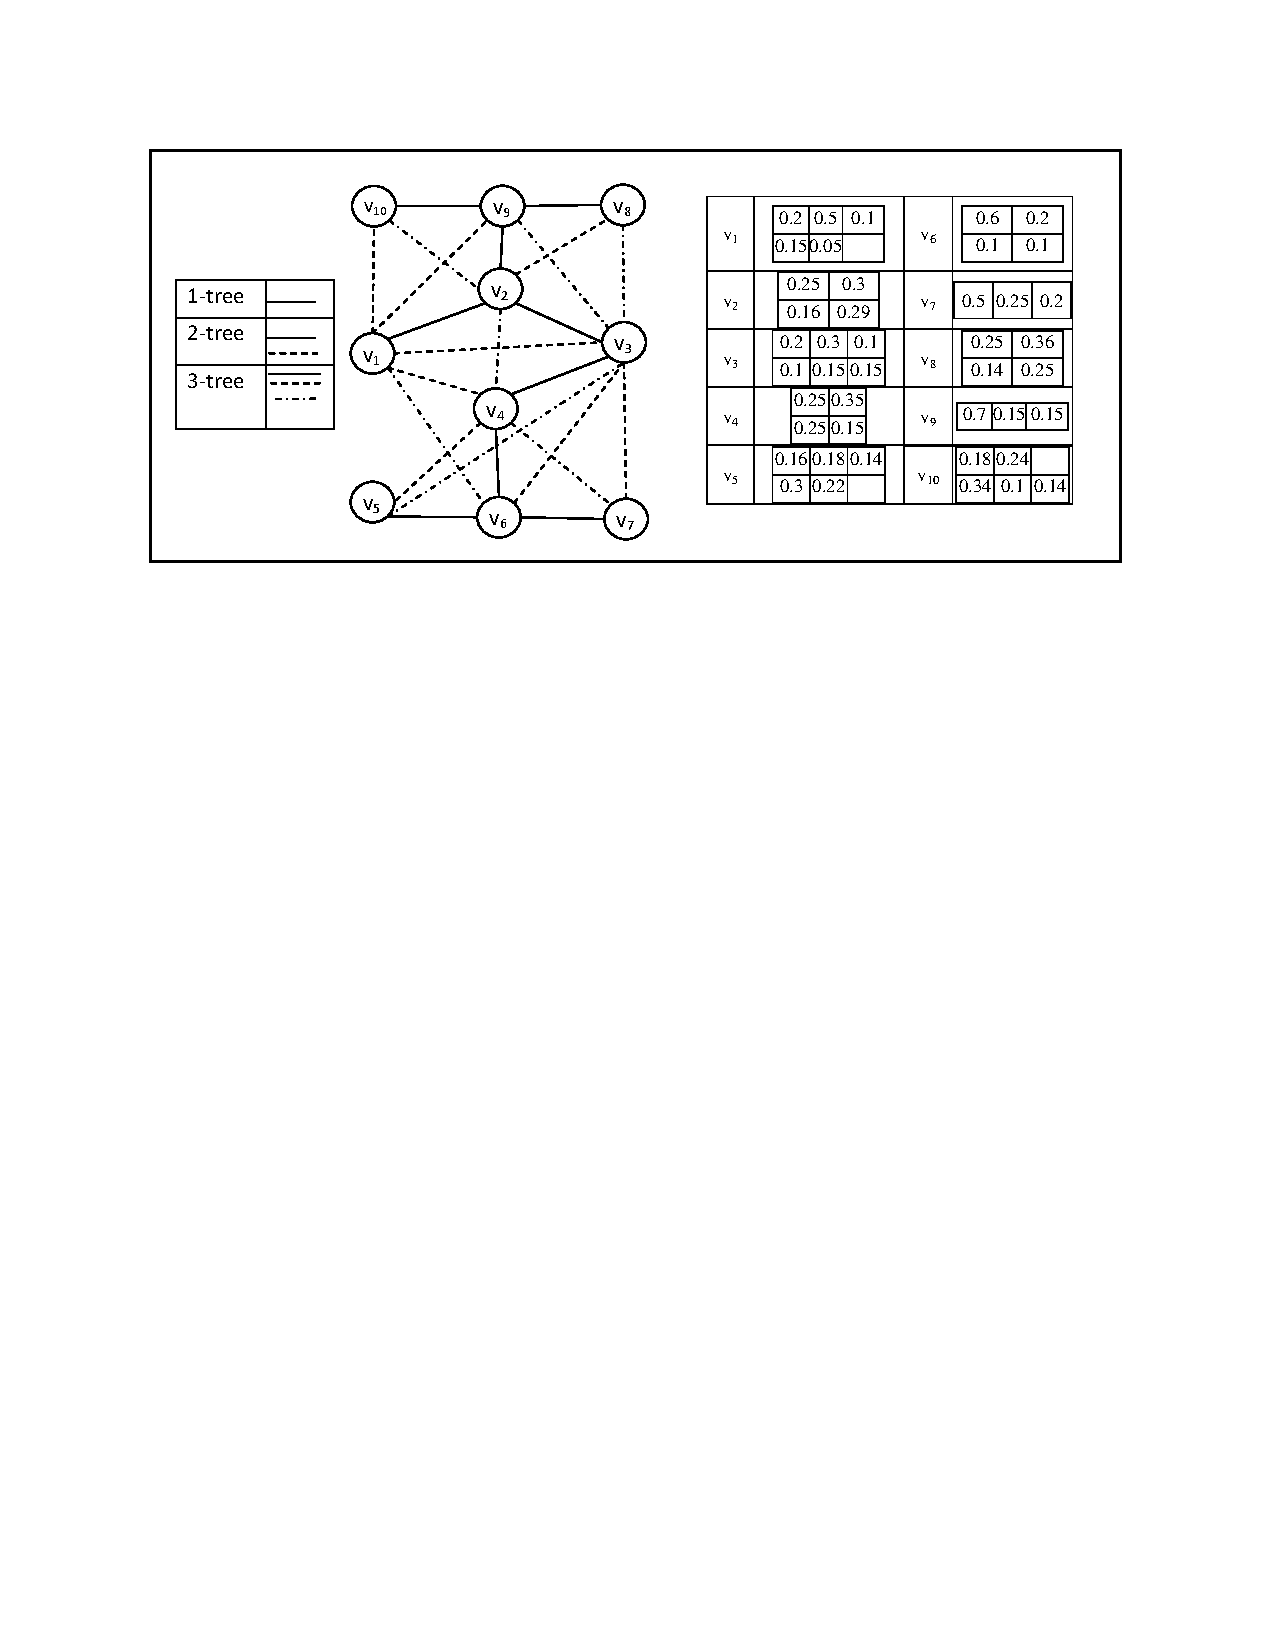
\includegraphics[width=3.8 in, height=2 in]{NetworkI_paper.pdf}
\caption{$G_{10}$}
\end{figure}
\end{frame}
%-----------------------------------------
\begin{frame}
\frametitle{Test Networks(Cont.)}
\vspace{-0.7em}
\begin{figure}[htbp]
\centering
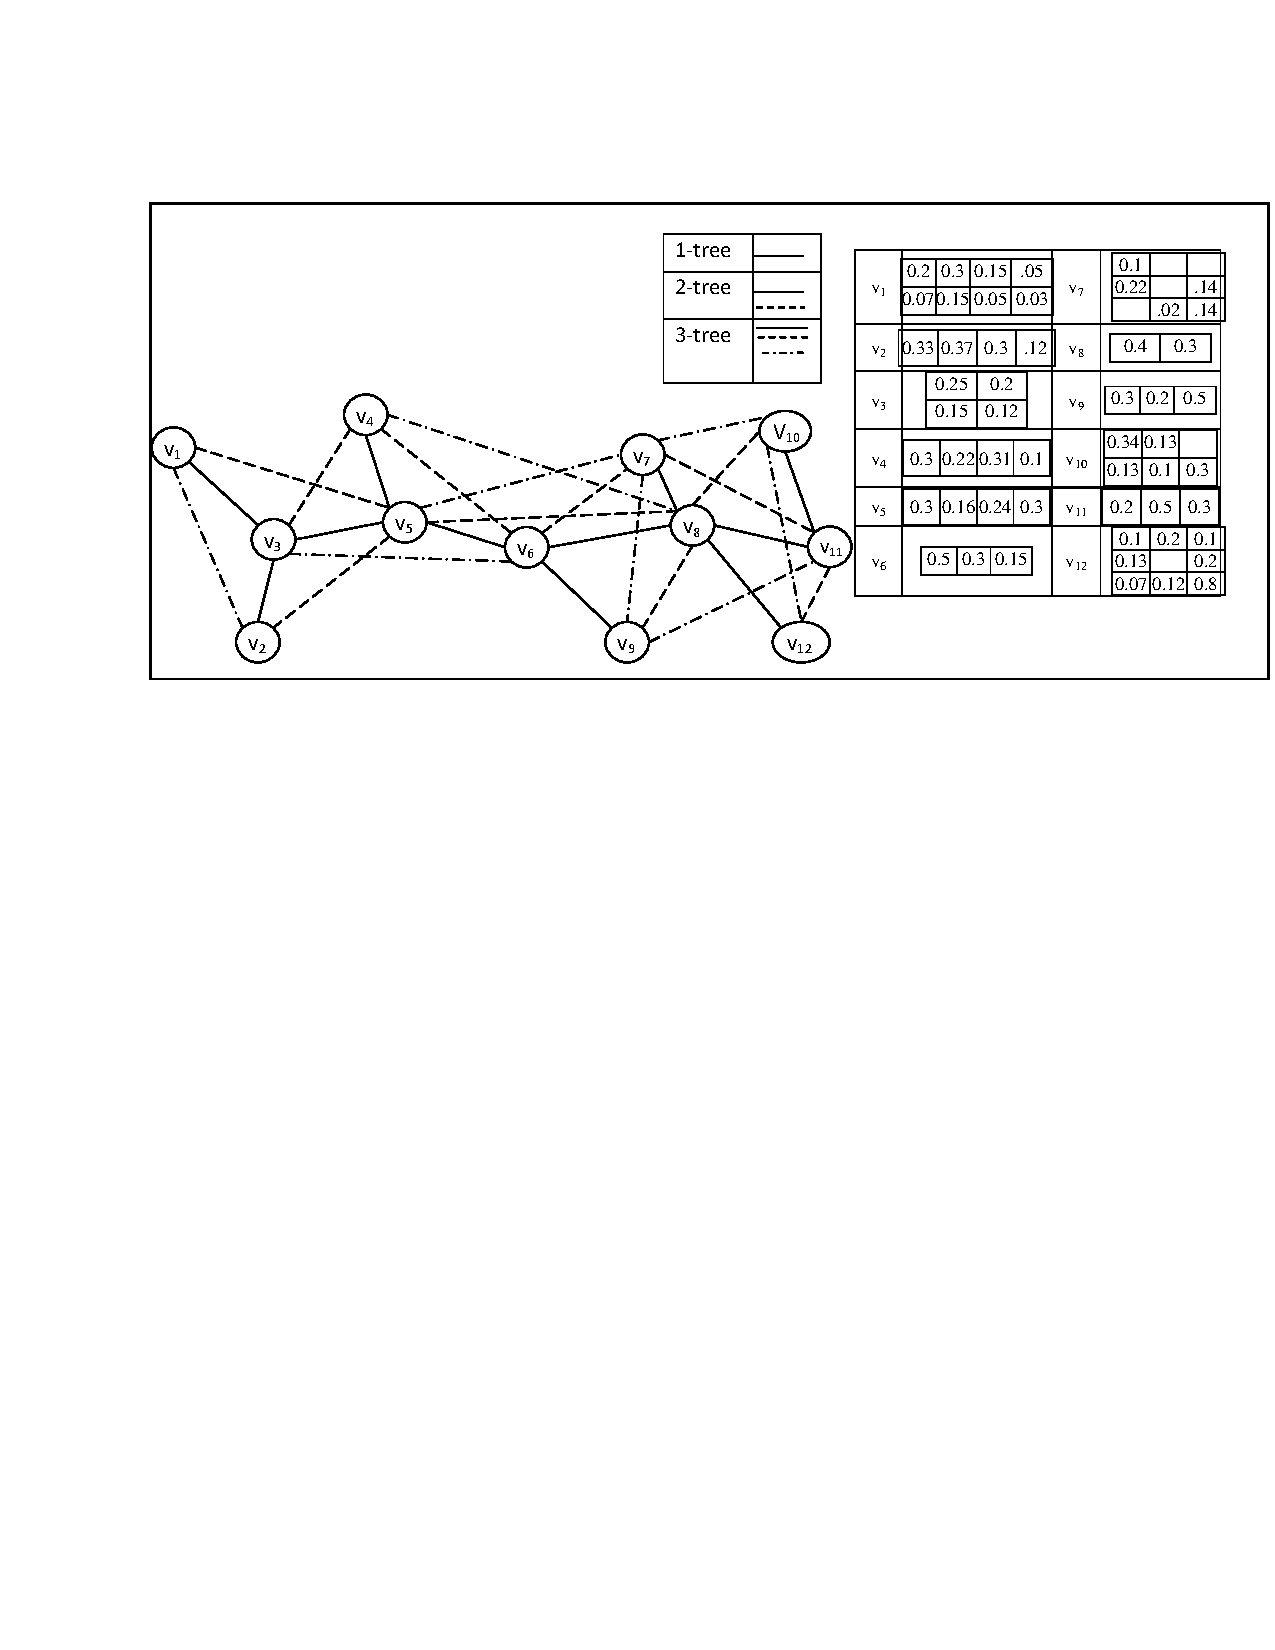
\includegraphics[width=3.8 in, height=1.2 in]{NetworkII.pdf}
\vspace{-1em}
\caption{$G_{12}$}
\end{figure}
\vspace{-1.5em}
\begin{figure}[htbp]
\centering
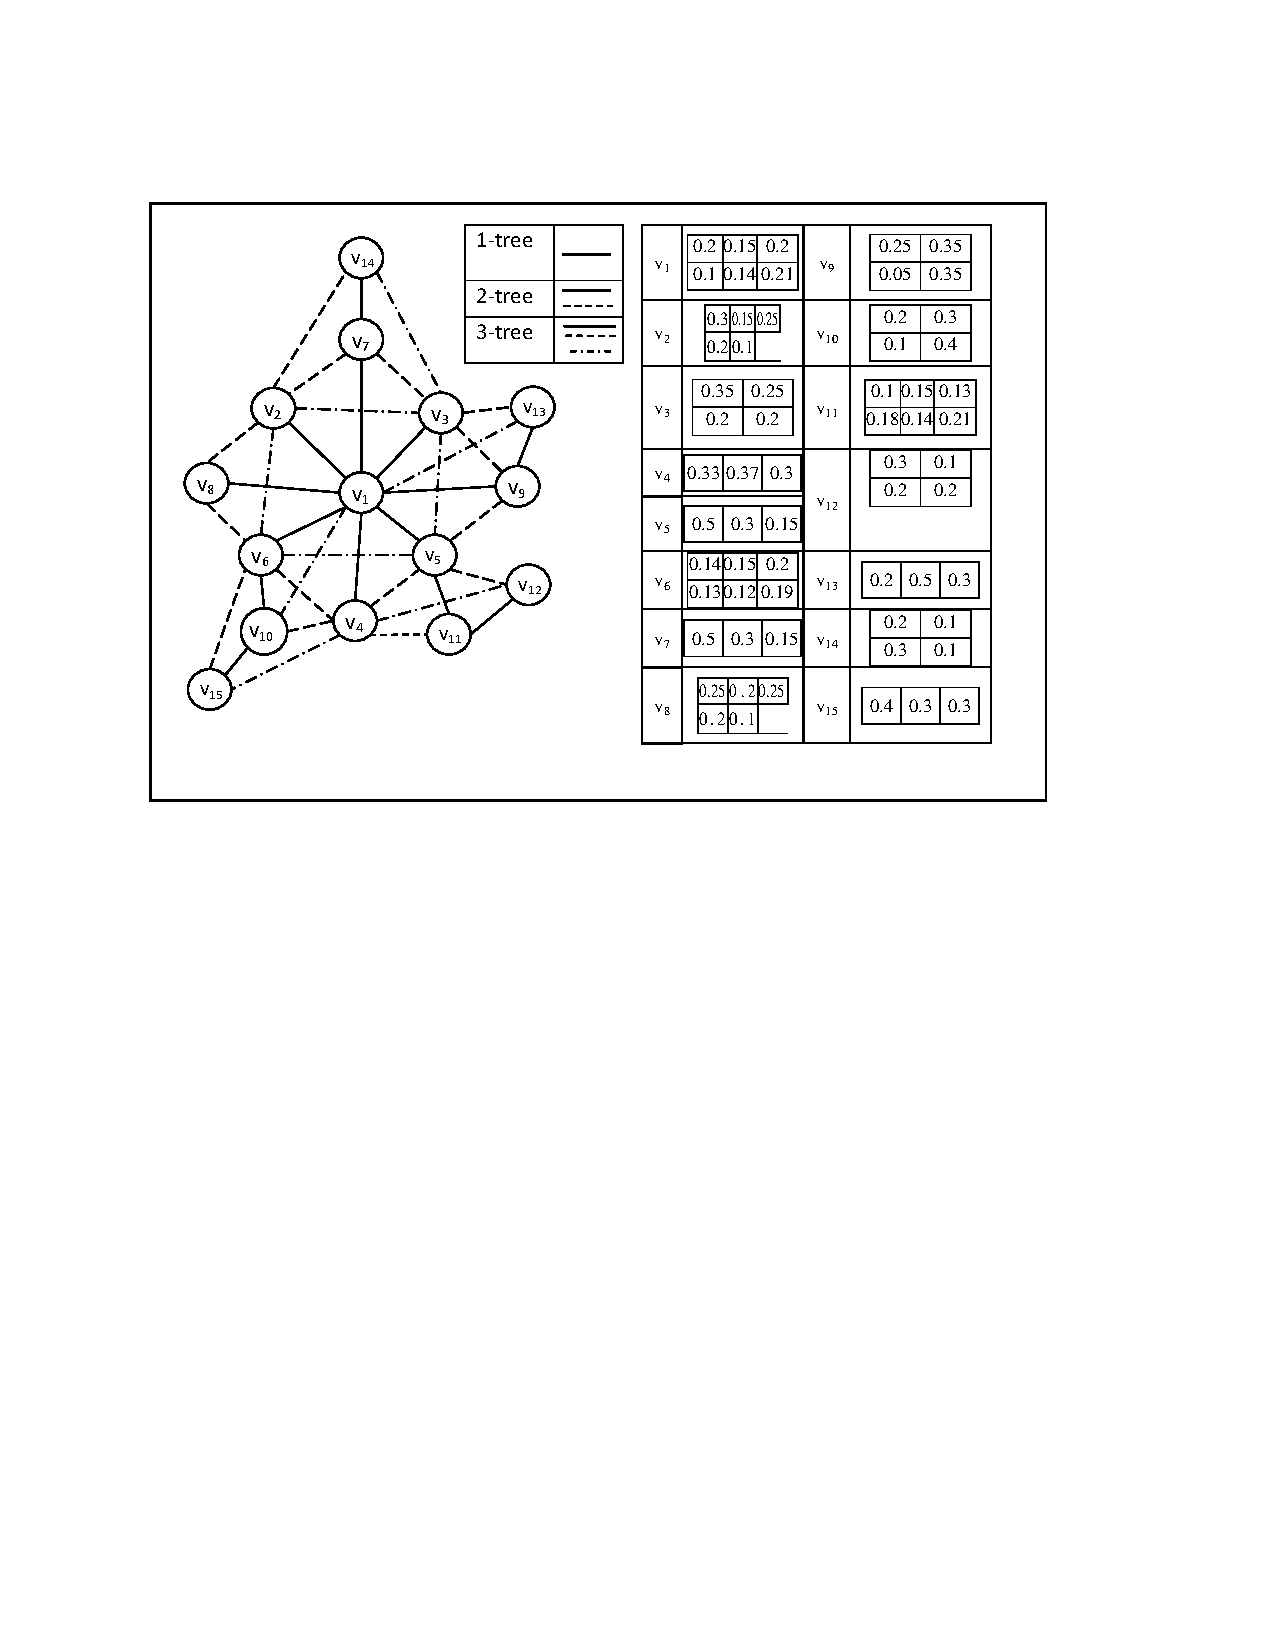
\includegraphics[width=3.8 in, height=1.5 in]{NetworkIII.pdf}
\vspace{-1em}
\caption{$G_{15}$}
\end{figure}
\end{frame}
%-----------------------------------------
\begin{frame}
\frametitle{Running Time}
\begin{table}[!htb]

    %\caption{Global caption}
    %\begin{minipage}{.5\linewidth}
   
      \centering
     \begin{tabular}{|c|c|c|c|}
     \hline
         k& Network $G_{10}$ & Network $G_{12}$ & Network $G_{15}$ \\
     \hline
     1&90& 130& 200 \\\hline
     2&1000 &1380&1480	\\\hline
3 &60000&875000&940000	 \\\hline
\end{tabular}
 \caption{Running time in milliseconds}
\label{Tab:runtym}
\end{table}

\end{frame}
%-----------------------------------------

%-----------------------------------------
\begin{frame}
\frametitle{Connectivity for different partial $k$-trees}
\begin{table}[!htb] 
      \centering
     \begin{tabular}{|c|c|c|c|}
     \hline
      k& Network $G_{10}$ & Network $G_{12}$ & Network $G_{15}$ \\
     \hline
      1 & 0.62&0.336& 0.82 \\\hline
2 &0.71 & 0.36& 0.99\\\hline
3 &0.75& 0.37& 1\\\hline
\end{tabular}
 \caption{Connectivity lower bounds using different partial $k$-trees}
 \label{Tab:acc}
\end{table}
\end{frame}
%-----------------------------------------
%-----------------------------------------
\begin{frame}
\frametitle{Effect of subgraph selection method}

\begin{figure}[!htb]
\begin{minipage}[]{.45\linewidth}
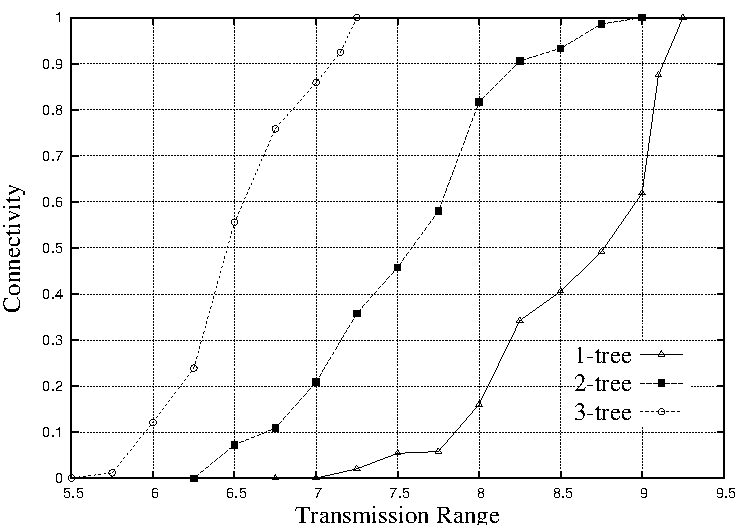
\includegraphics[width=2.2 in, height=2.2 in]{Random-eps-converted-to.pdf}
 \caption{ Connectivity versus transmission range with random subgraph selection
}
\label{fig:res}
\end{minipage}
\begin{minipage}{.45\linewidth}
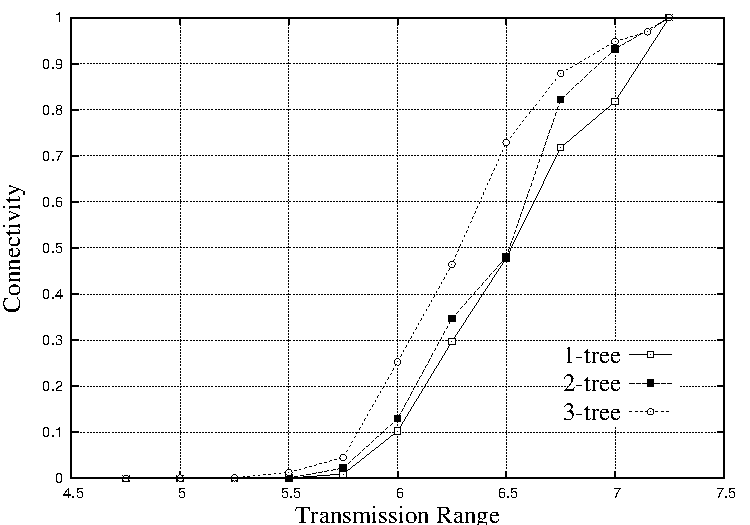
\includegraphics[width=2.2 in, height=2.2 in]{Selective-eps-converted-to.pdf}
 \caption{ Connectivity versus transmission range with greedy subgraph selection
}
\label{fig:ges}
 \end{minipage}
\end{figure}

\end{frame}
%-----------------------------------------
\section{$\ARCONN$ and $\SRCONN$ problems}
%-----------------------------------------

%\subsection{Algorithms for $\ARCONN$ and $\SRCONN$}
%\subsection{Simulation Results for $\ARCONN$ and $\SRCONN$}
\begin{frame}
\frametitle{$\ARCONN$ and $\SRCONN$ problems}
\begin{itemize}
\item $\ARCONN$ State types
\item merging $\ARCONN$ state types
\item removing bad states from $\ARCONN$ state types
\item Simulation Results for $\ARCONN$ problem.
\item $\SRCONN$ State types
\item merging $\SRCONN$ state types
\item removing bad states from $\SRCONN$ state types
\item Simulation Results for $\SRCONN$ problem.
\end{itemize}
\end{frame}


\begin{frame}
\frametitle{$\ARCONN$ state types}

\centerline{
$AR\mbox{-}type(S)=\{V_{1,b(V_1)}^{Loc(V_1)}, V_{2,b(V_2)}^{Loc(V_2)}, \ldots, V^{Loc(V_r)}_{r,b(V_r)} \}$}
\begin{example}
\normalfont
In the figure, denote by $G_{v_i,1}$, the graph induced on nodes $\{v_a,v_b,v_i,v_j,v_k\}$. Assume that $\{v_b\}\in V_{sense}$ and $\{v_a,v_i,v_j,v_k\} \in V_{relay}$. Suppose that state $S$ of the figure is a possible network state of $G_{v_i,1}$. Then $AR\mbox{-}type(S)=\big \{\{v_i\}_1^{(1)},\{v_j,v_k\}_0^{(2,3)}\big\}$. Here, the indicator $b(\{v_i\})=1$ since $v_b$ is a sensor node connected to $v_i$ in $S$. 
\end{example}

\begin{figure}[!htb]
\begin{minipage}[]{0.45\linewidth}
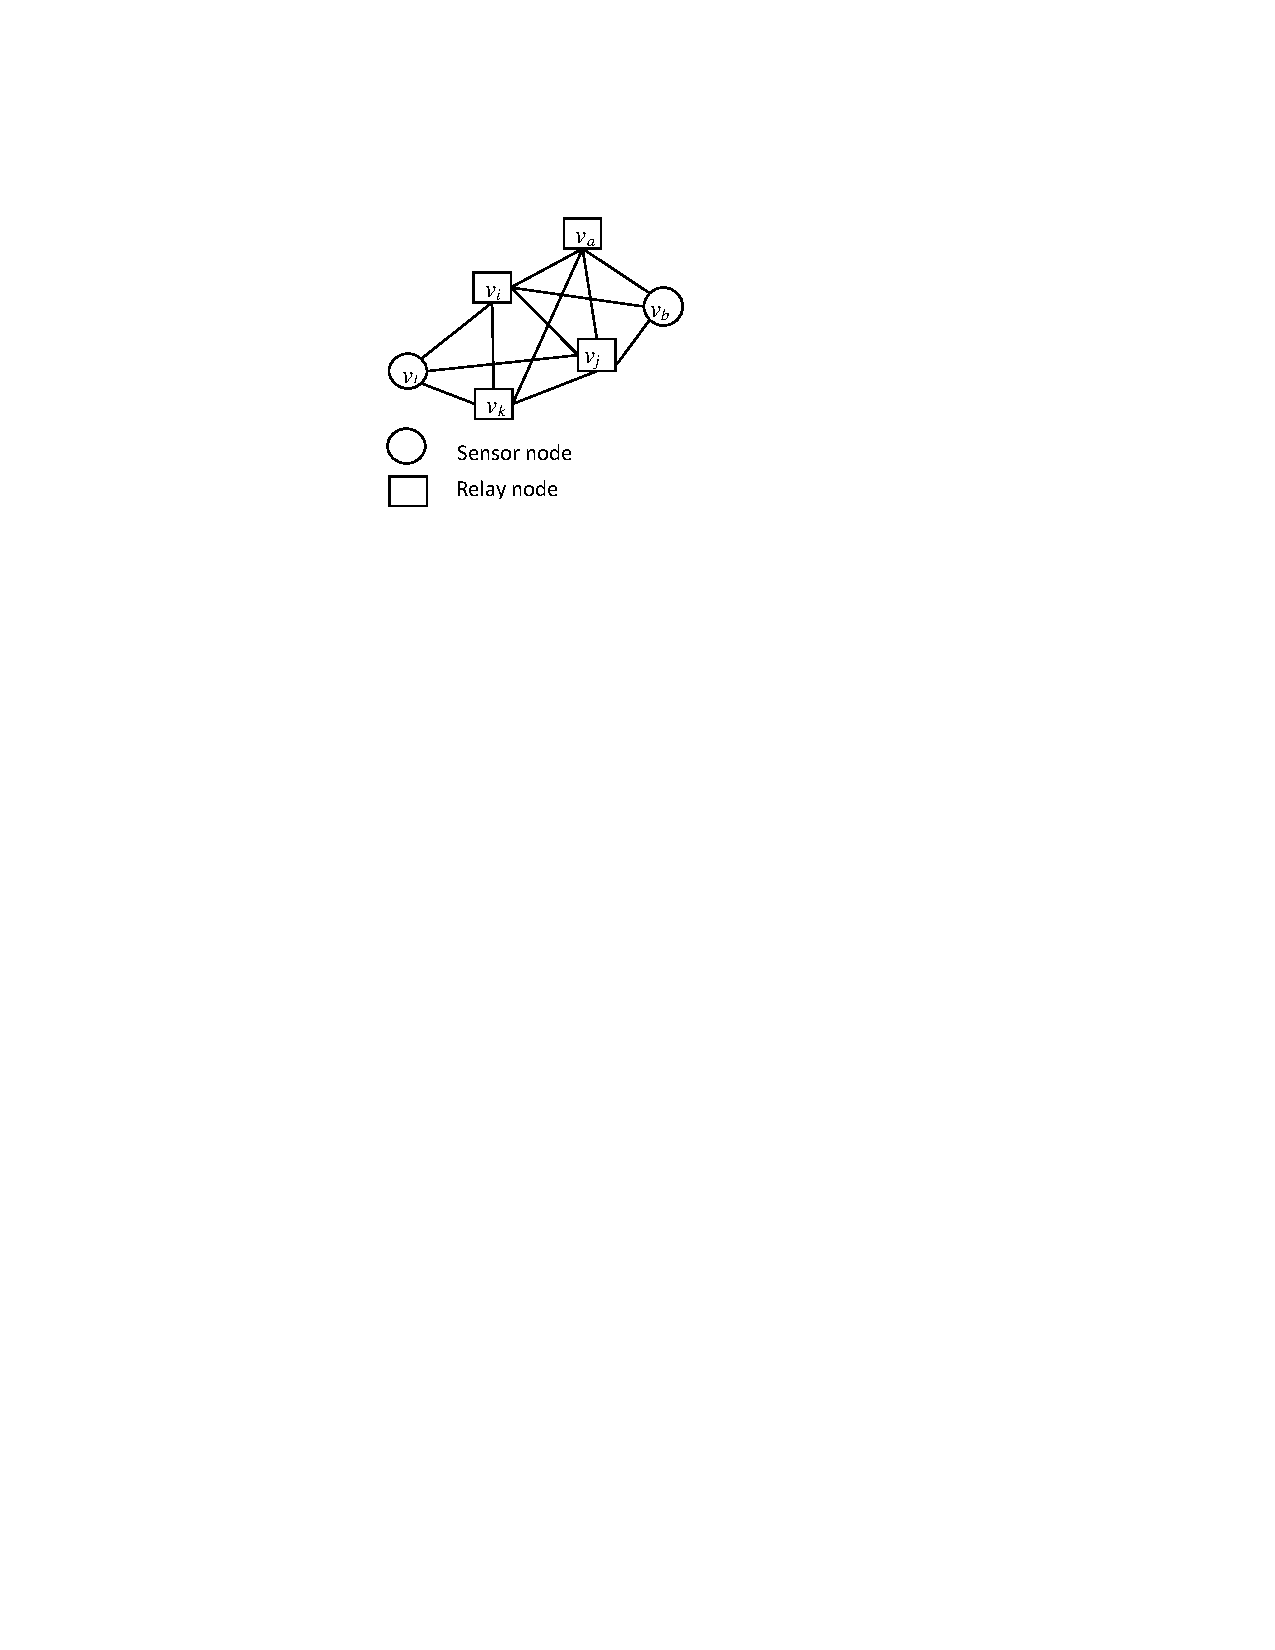
\includegraphics[width=1.5 in, height=1 in]{Ch5f2.pdf}
\caption{A fragment of a 3-tree}
\label{fig:sttype1}
\end{minipage}
\begin{minipage}{0.45\linewidth}
\nwline
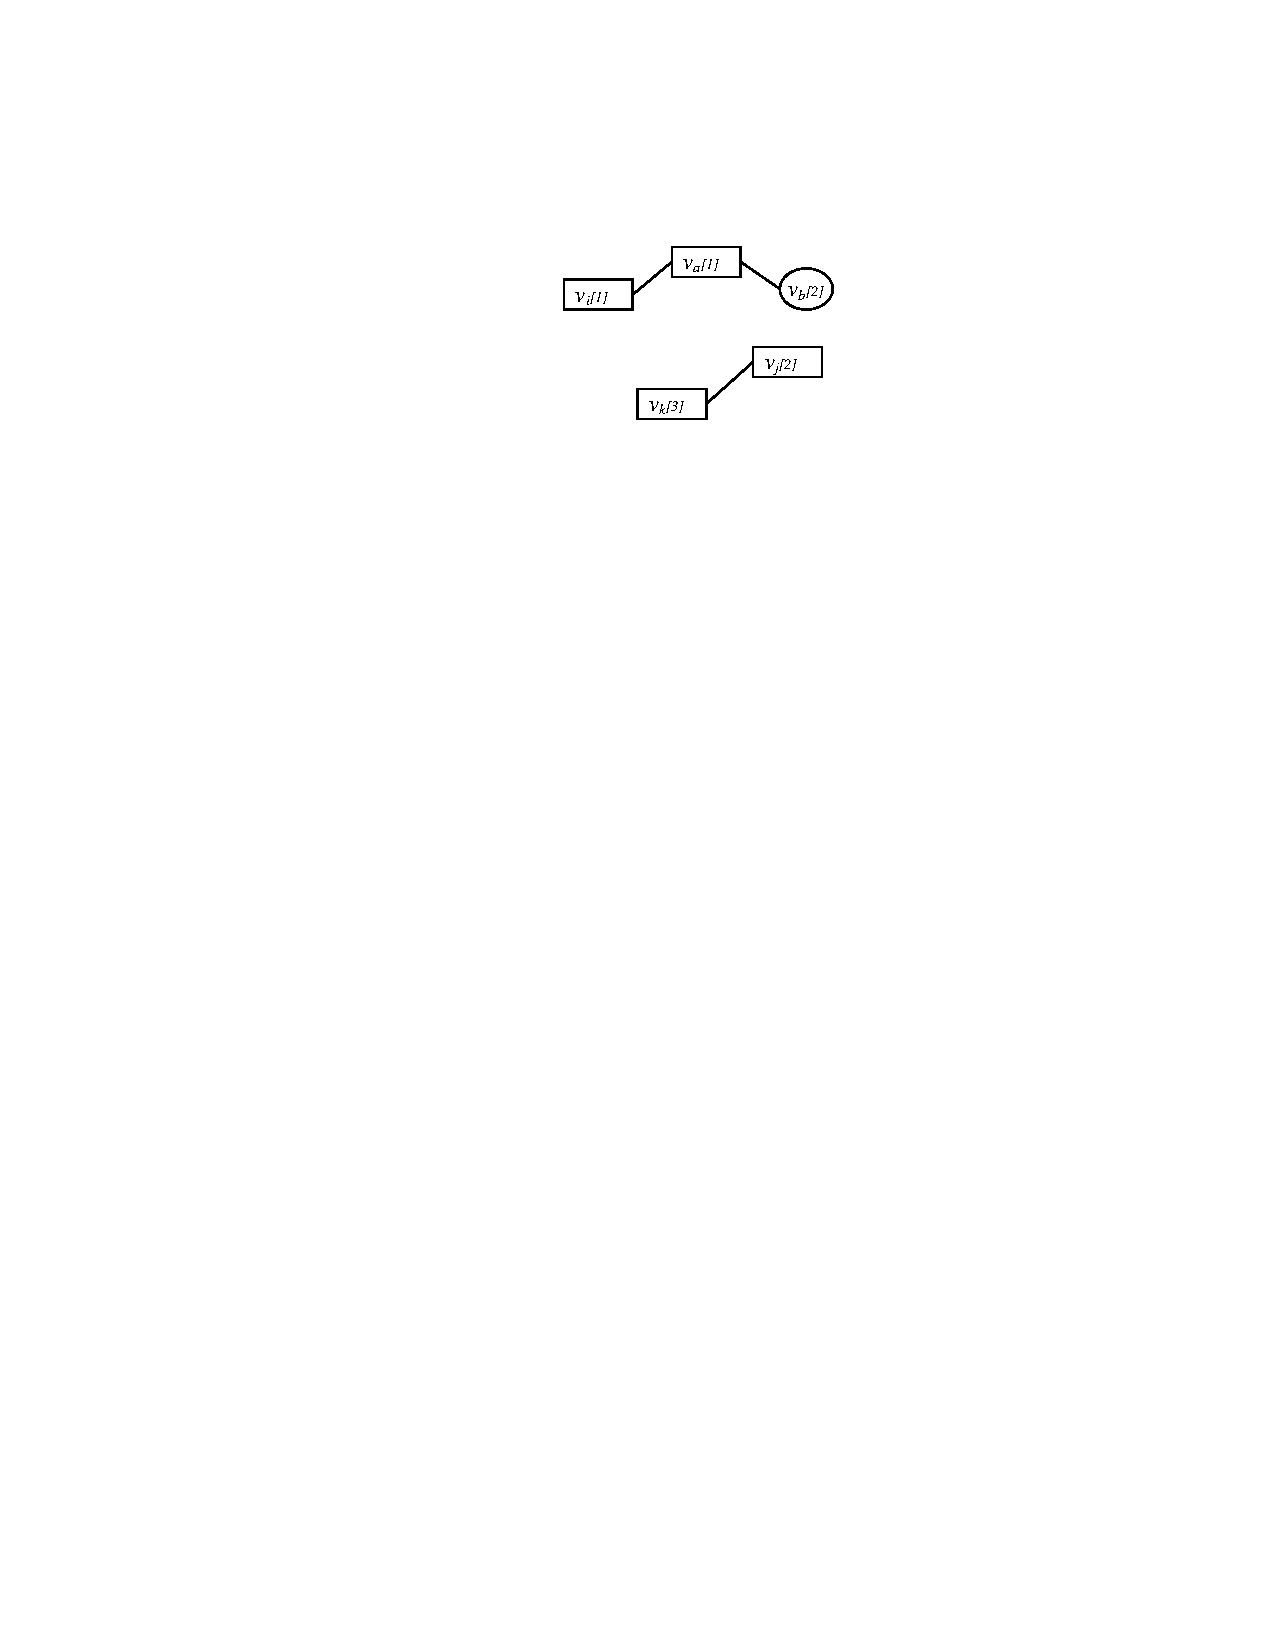
\includegraphics[width=1.2 in, height=1 in]{Ch5f2_1.pdf}
\caption{A state $S$ on $\{v_a,v_b,v_i,v_j,v_k\}$}
\label{fig:sttype1_node}
\end{minipage}
\end{figure}
\end{frame}
%-----------------------------------------

%-----------------------------------------
\begin{frame}
\frametitle{Merging State types}
\begin{figure}
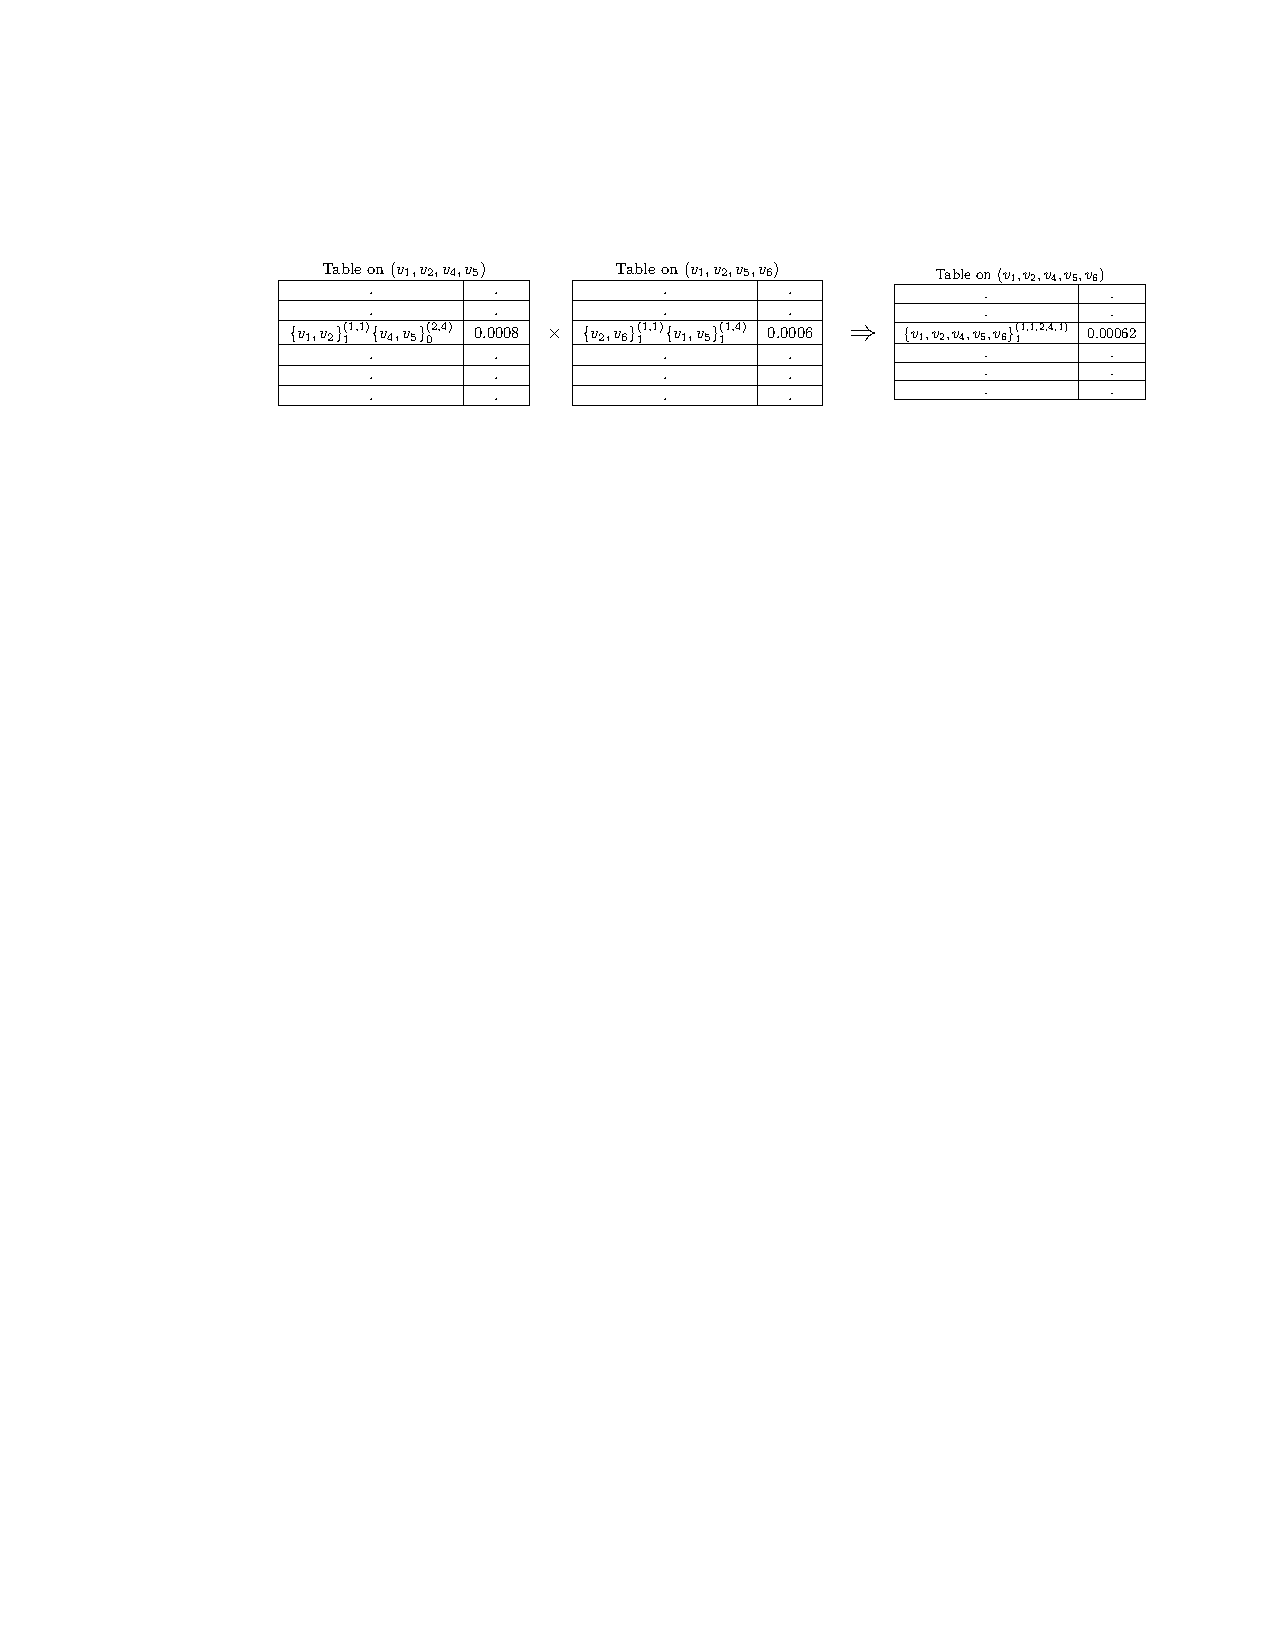
\includegraphics[scale=0.8]{part.pdf}
\caption{Merging two tables}
\end{figure}
\end{frame}
%-----------------------------------------

%-----------------------------------------
\begin{frame}
\frametitle{Removing Bad State Types}
\begin{itemize}

\item For the $\ARCONN$ problem, a state $S$ of the subgraph $G_{v_i,base}$ reduced onto the $k$-clique $K_{v_i,base}$.
\item $S$ is considered bad if node $v_i$ appears as a singleton part and the indicator $b({v_i})=1$.
\item The algorithm removes all such bad state types from $T_{v_i,base}$.

\end{itemize}
\end{frame}
%-----------------------------------------
\begin{frame}
\frametitle{Running Time of $\ARCONN$}
\begin{center}
\begin{theorem}\normalfont In the $\ARCONN$ algorithm we have\label{thm:rt}
\begin{enumerate}
\item The maximum length of any table is $O(B_kl_{max}^k2^k)$ 
\item The worst case running time is $O(n(B_kl_{max}^k2^k)^2)$
\end{enumerate}
\end{theorem}
\end{center}
\end{frame}
%-----------------------------------------
\begin{frame}
\frametitle{Simulation Results}
\begin{itemize}
\item Test Networks
\item Running time
\item Effects of Adding Relay nodes
\end{itemize}
\end{frame}
%-----------------------------------------

%-----------------------------------------
\begin{frame}
\frametitle{Test Networks}
\vspace{-0.5em}
\begin{figure}[!htb]
\begin{minipage}{.8\linewidth}
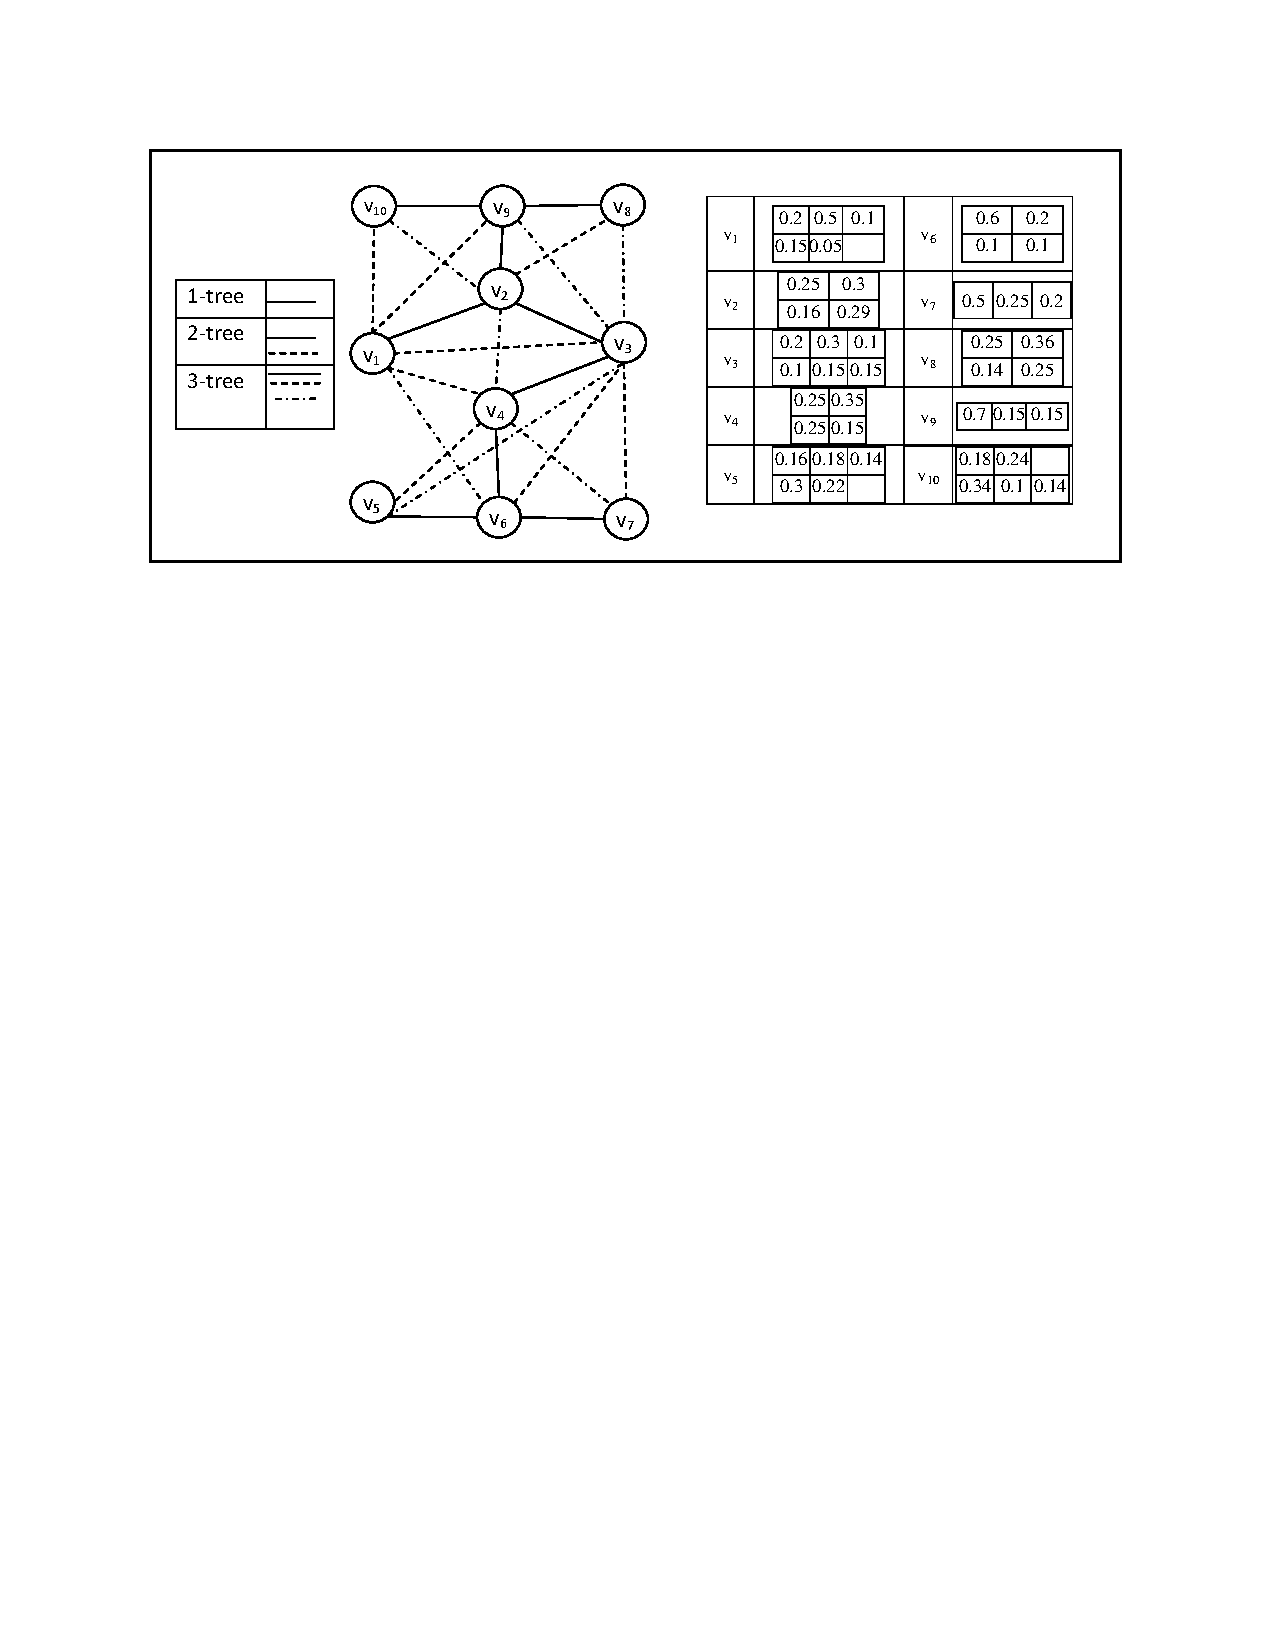
\includegraphics[width=4 in, height=1.2 in]{NetworkI_paper.pdf}
\caption{Network $G_{10}$}
\label{fig:netI1}
\end{minipage}
\begin{minipage}{.8\linewidth}
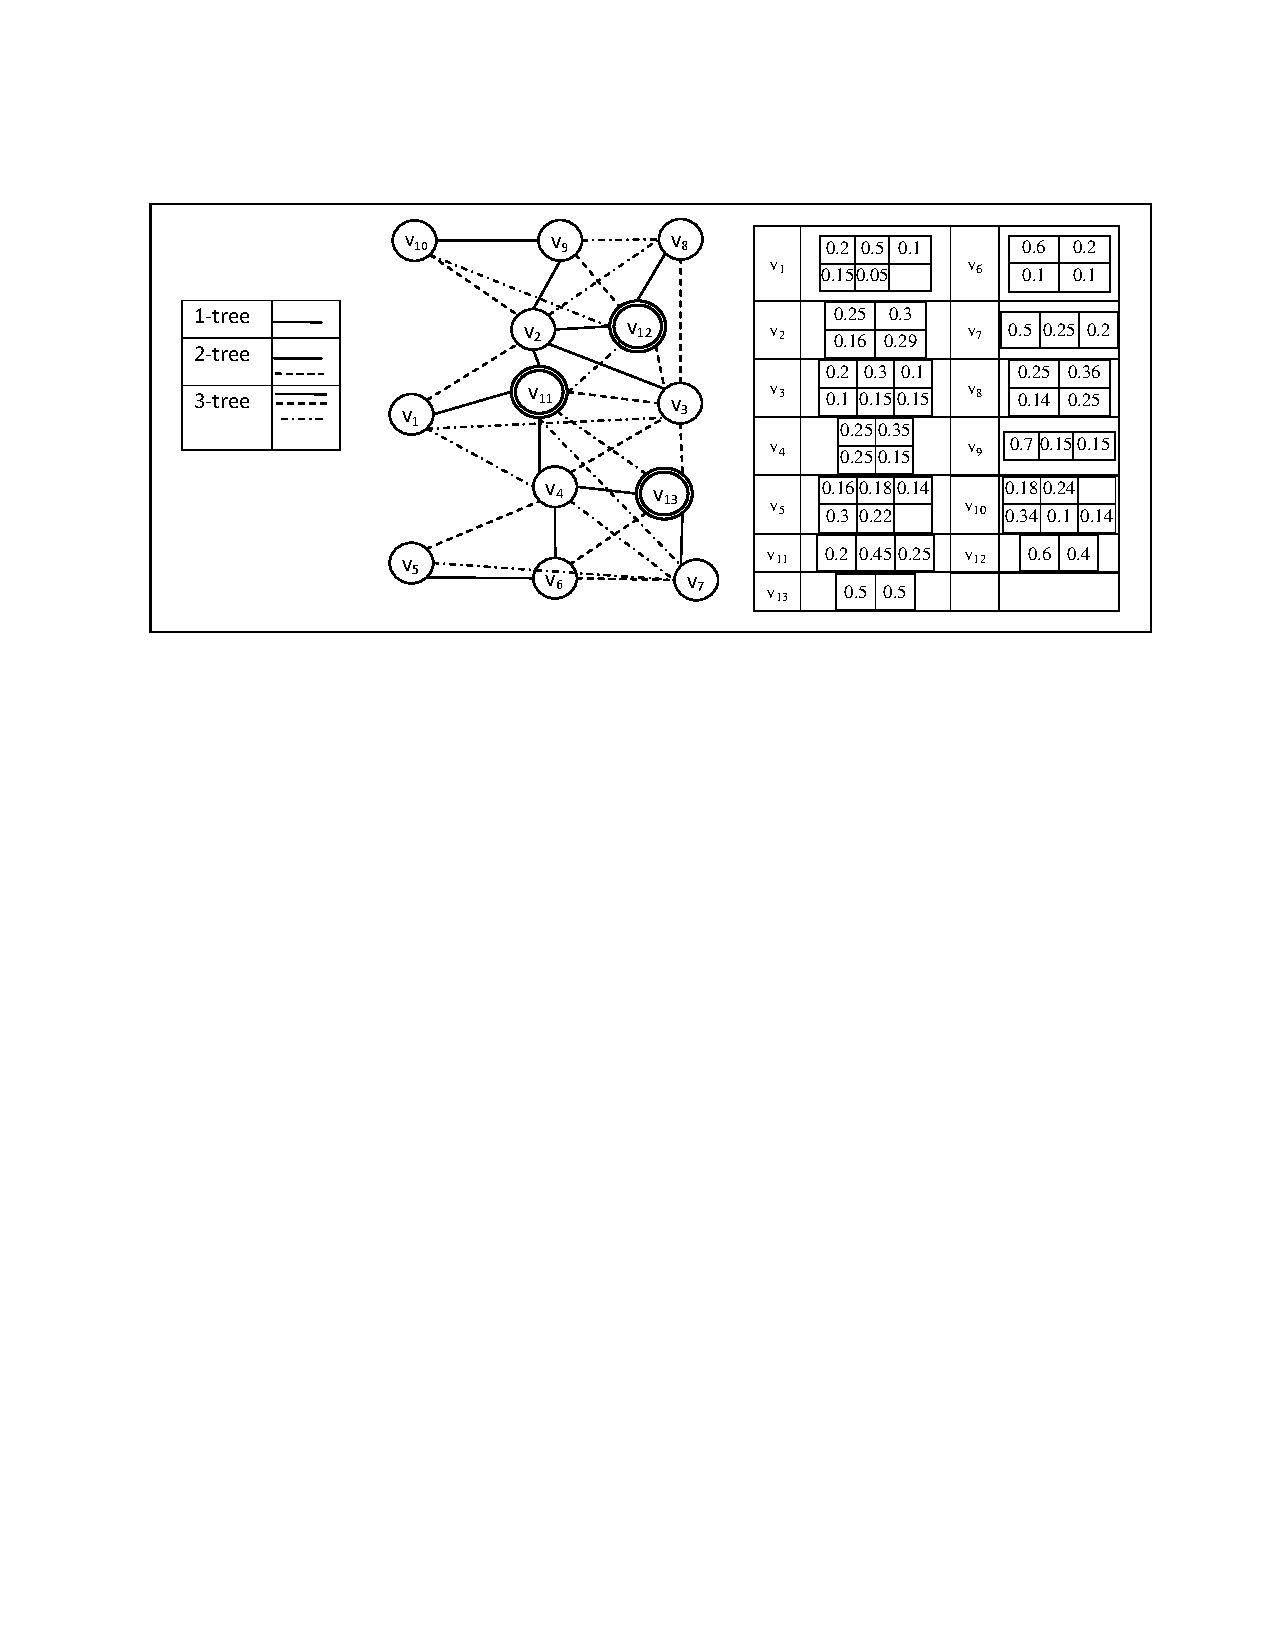
\includegraphics[width=4 in, height=1.2 in]{NetworkI_paper_Relay.pdf}
\vspace{-0.7 cm}
\caption{Network $G_{10,3}$}
\label{fig:netIR}
\end{minipage}
\end{figure}

\end{frame}
%-----------------------------------------

%-----------------------------------------
\begin{frame}
\frametitle{Running Time}
\begin{table}[!htb]
    %\caption{Global caption}
    \begin{minipage}{1\linewidth}
   
      \centering
     \begin{tabular}{|c|c|c|}
     \hline
         k& Network $G_{10}$ &Network $G_{10,3}$\\
     \hline
     1&90& 110 \\\hline
     2&1000 &6000	\\\hline
3 &6000&8000	 \\\hline
\end{tabular}
 \caption{Running time in milliseconds}
\label{Tab:rtym1}
    \end{minipage}
\end{table}

\end{frame}
%-----------------------------------------

%-----------------------------------------
\begin{frame}
\frametitle{Effect of adding relay nodes}

\begin{table}[!htb]
  \centering
 \begin{minipage}{.5\linewidth}
     \begin{tabular}{|c|c|c|}
     \hline
     k & Network $G_{10}$ & Network $G_{10,3}$  \\
     \hline
      1 & 0.30 & 0.86 \\\hline
	  2 & 0.54 & 0.96\\\hline
	  3 &0.60 & 0.98 \\\hline
\end{tabular}
    \end{minipage}
     \caption{Connectivity with respect to $k$}
      \label{Tab:SRC}   
\end{table}
\end{frame}
%-----------------------------------------

%-----------------------------------------
\begin{frame}
\frametitle{Effect of adding relay nodes for various node $R_{tr}$:}
\begin{itemize}
\item Each obtained curve exhibits a notable monotonic increasing behaviour as $R_{tr}$ increases. 
\item This behaviour is due to the appearance of more edges, and the potential increase in the probability of each edge as $R_{tr}$ increases. 
\item Increasing $R_{tr}$, however, requires increasing node energy consumption.
\item  To achieve a desired $Conn(G)$ value, a designer may utilize the obtained curves to assess the merit of increasing $R_{tr}$ versus deploying more relay nodes.
\end{itemize}
\begin{figure}[!htb]
\begin{minipage}{.9\linewidth}
\end{minipage}
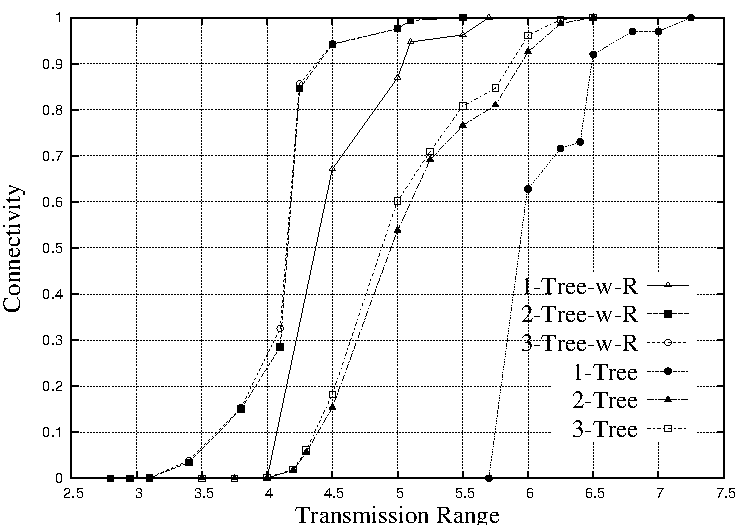
\includegraphics[width=4 in, height=1.35 in]{NetworkI_woR-eps-converted-to.pdf}
\caption{Connectivity versus transmission range}
\label{Fig:NWOR}
\end{figure}

\end{frame}
%--------------
\begin{frame}
\frametitle{The $\SRCONN$ State Types}


\centerline{
$SR\mbox{-}type(S)=\{V_{1,c(V_1)}^{Loc(V_1)}, V_{2,c(V_2}^{Loc(V_2)}, \ldots, V^{Loc(V_r)}_{r,c(V_r} \}$}

\begin{example}
\normalfont
 In the figure, denote by  $G_{v_i,1}$, the graph induced on nodes $\{v_a,v_b,v_i,v_j,v_k\}$. Assume that $\{v_b,v_i\}\in V_{sense}$ and $\{v_a,v_j,v_k\} \in V_{relay}$. Suppose that state $S$ of the figure is a possible network state of $G_{v_i,1}$. Then $SR\mbox{-}type(S)=\big \{\{v_i\}_2^{(1)},\{v_j,v_k\}_0^{(2,3)}\big\}$. Here, the count $c(\{v_i\})=2$ since both of $v_i$ and $v_b$ are sensor nodes.
 
\end{example}
\vspace*{-0.4 cm}
\begin{figure}[!htb]
\begin{minipage}[]{0.45\linewidth}
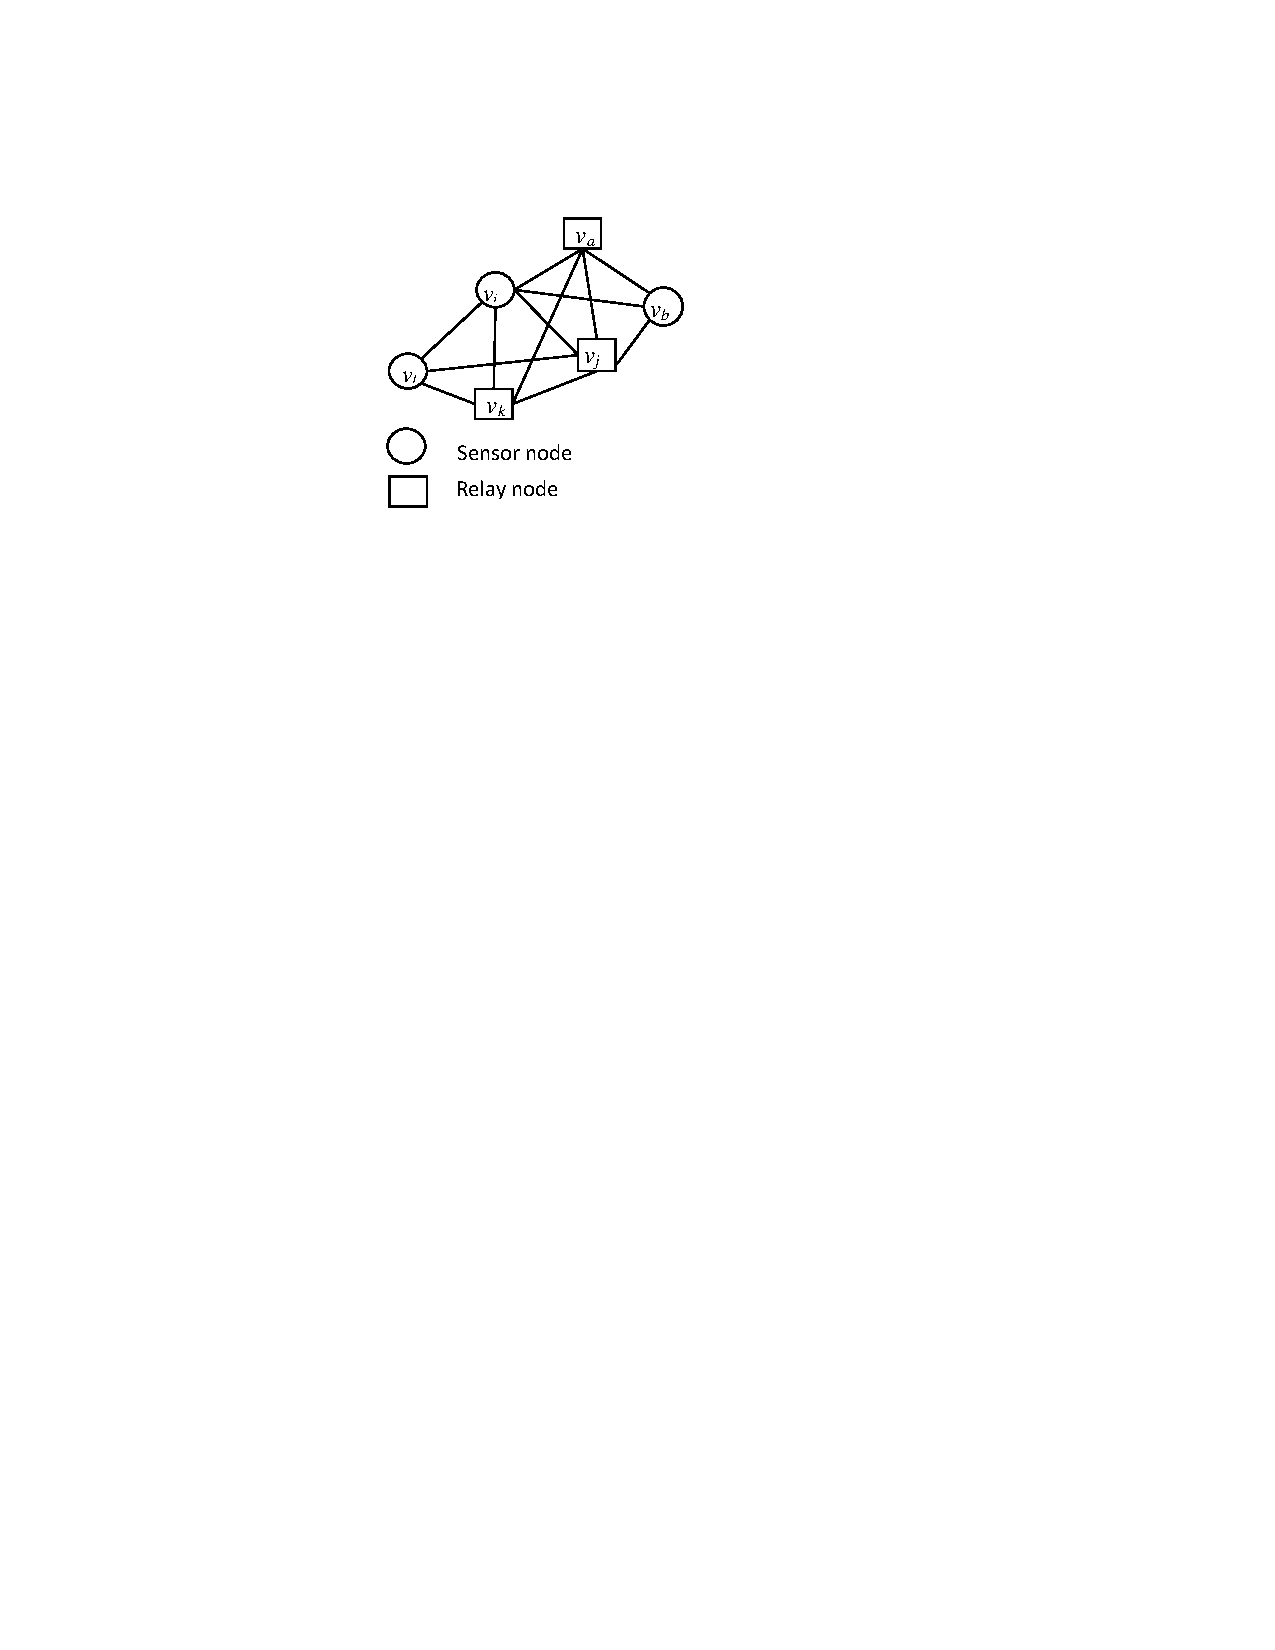
\includegraphics[width=1.5 in, height=1 in]{Ch5f3.pdf}
\caption{A 3-tree fragment}
\label{fig:sttype2}
\end{minipage}
\begin{minipage}{0.45\linewidth}
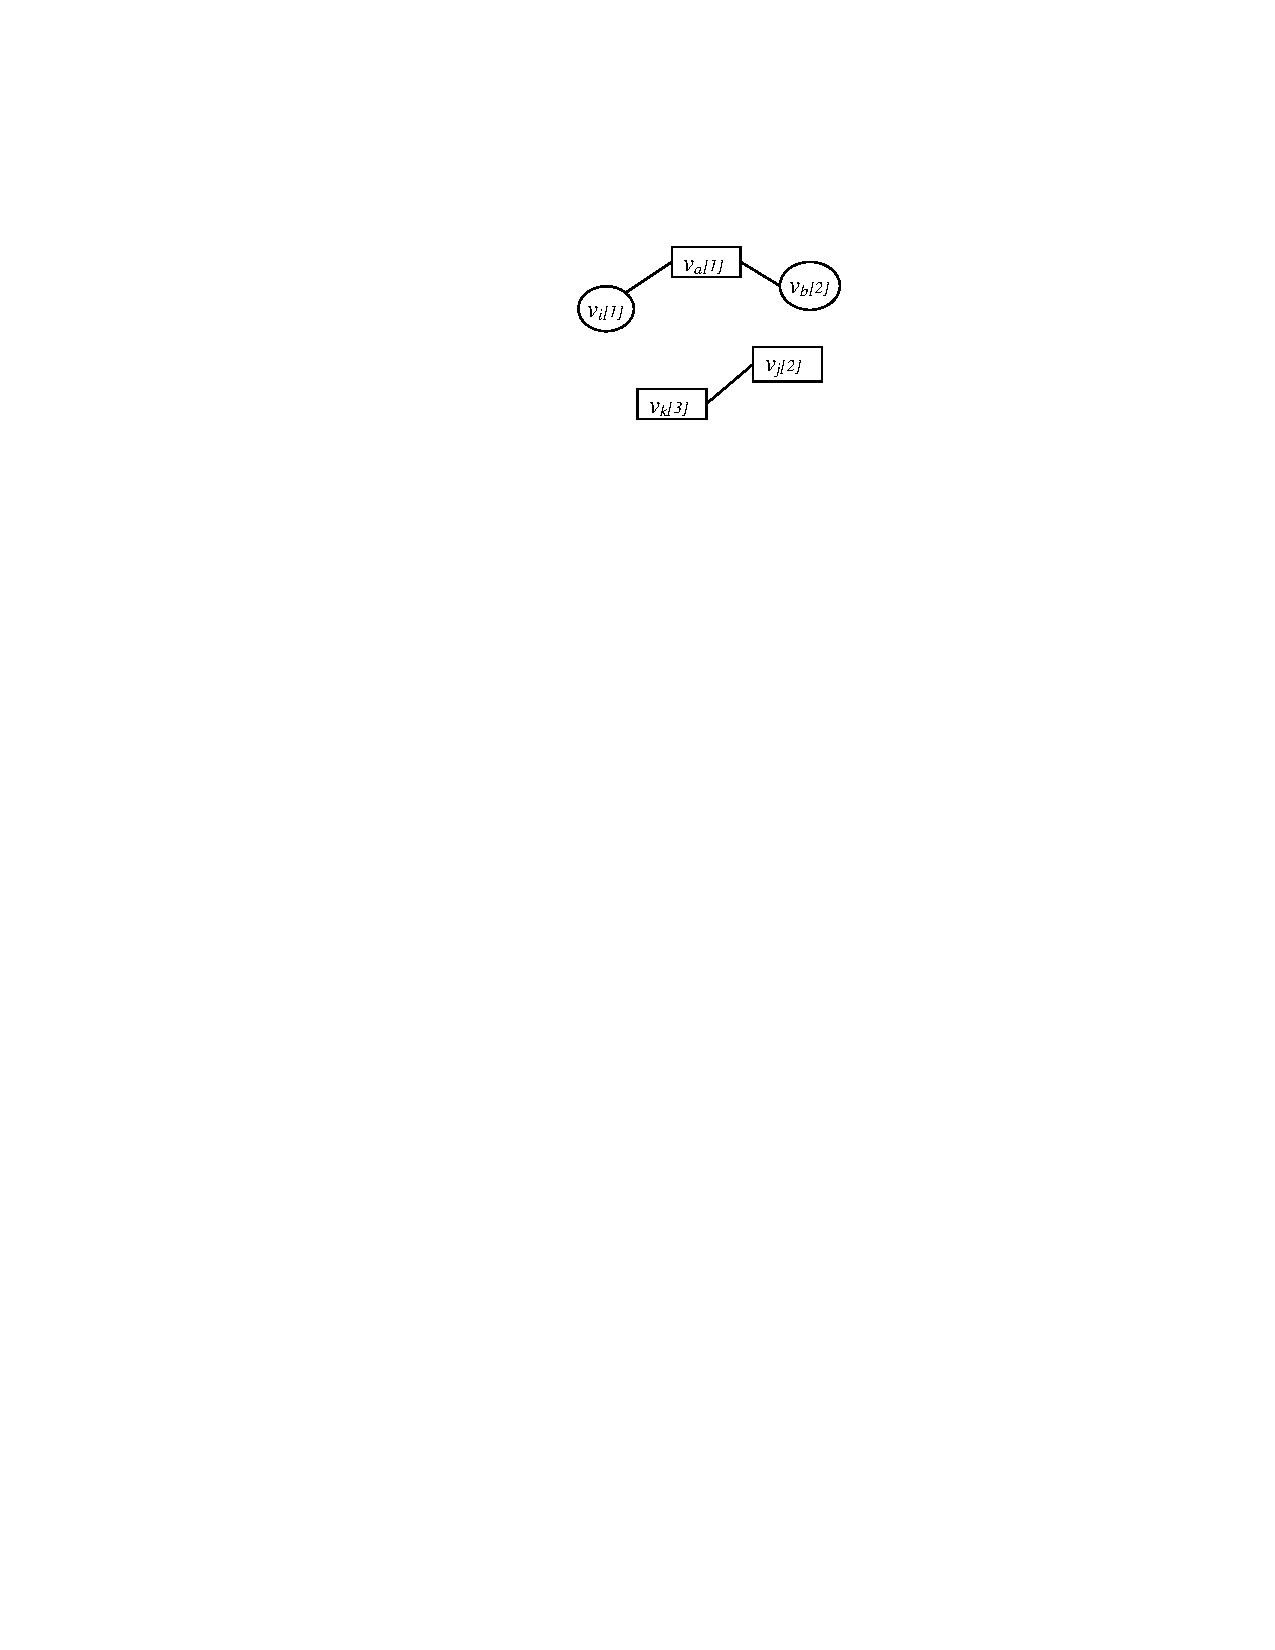
\includegraphics[width=1.2 in, height=1 in]{Ch5f3_1.pdf}
\caption{A state $S$ on $\{v_a,v_b,v_i,v_j,v_k\}$}
\label{fig:sttype2_node}
\end{minipage}
\end{figure}

\end{frame}
%-----------------------------------------
%--------------
\begin{frame}
\frametitle{Merging State types}
\begin{figure}
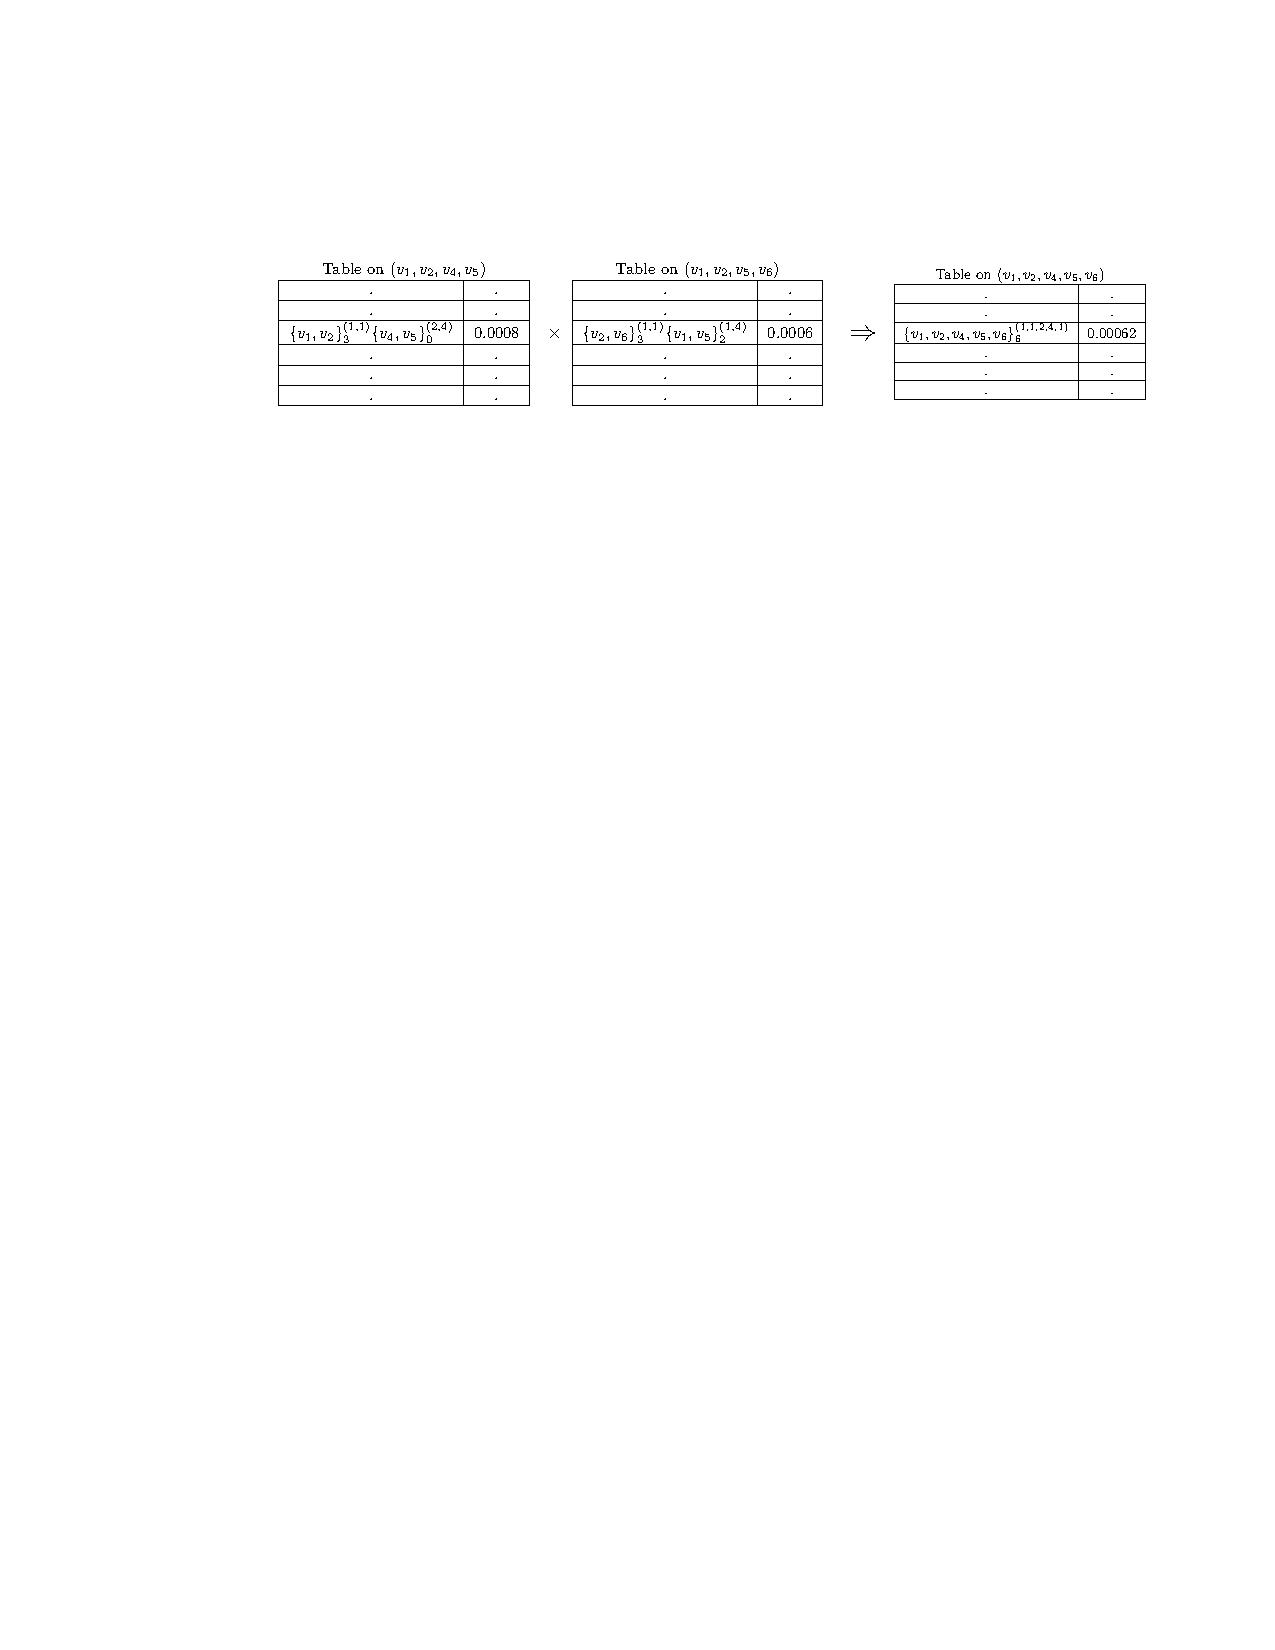
\includegraphics[scale=0.8]{partition1.pdf}
\caption{Merging two tables}
\end{figure}
\end{frame}
%-----------------------------------------
%--------------
\begin{frame}
\frametitle{Bad State Types}
\begin{itemize}

\item For the $\SRCONN$ problem, a state $S$ of the subgraph $G_{v_i,base}$ reduced onto the $k$-clique $K_{v_i,base}$.
\item $S$ is considered bad if node $v_i$ appears as a singleton part and the indicator $c({v_i})\geq 1$.
\item The algorithm removes all such bad state types from $T_{v_i,base}$.

\end{itemize}
\end{frame}
\begin{frame}
\frametitle{Running Time $\SRCONN$}
\begin{theorem}\normalfont In the $\SRCONN$ algorithm we have\label{thm:rt1}
\begin{enumerate}
\item The maximum length of any table is $O(B_kl_{max}^kn_{req}^k)$ 
\item The worst case running time is $O(n(B_kl_{max}^kn_{req}^k)^2)$
\end{enumerate}
\end{theorem}
\end{frame}
%-----------------------------------------
\begin{frame}
\frametitle{$\SRCONN$ Simulation Results}
A designer has at least 3 options to achieve a minimum required $Conn(G,n_{req})$ value:

\begin{itemize}
\item tuning the $n_{req}$ parameter,
\item tuning node transmission range $R_{tr}$, and
\item tuning the number of deployed relay nodes.
\end{itemize}
\end{frame}


\begin{frame}
\frametitle{Effect of varying $n_{req}$} 
\begin{itemize}
\item Figure illustrates the achieved $Conn(G,n_{req})$ as $n_{req}$ varies in the range $[1,10]$.
\item Figure illustrates the achieved $Conn(G,n_{req})$ as $n_{req}$ varies in the range $[1,10]$, and $R_{tr}$ varies in the range $[2.5,5.5]$.

\end{itemize}
\begin{figure}[!htb]
\begin{minipage}{0.5\linewidth}
\centering
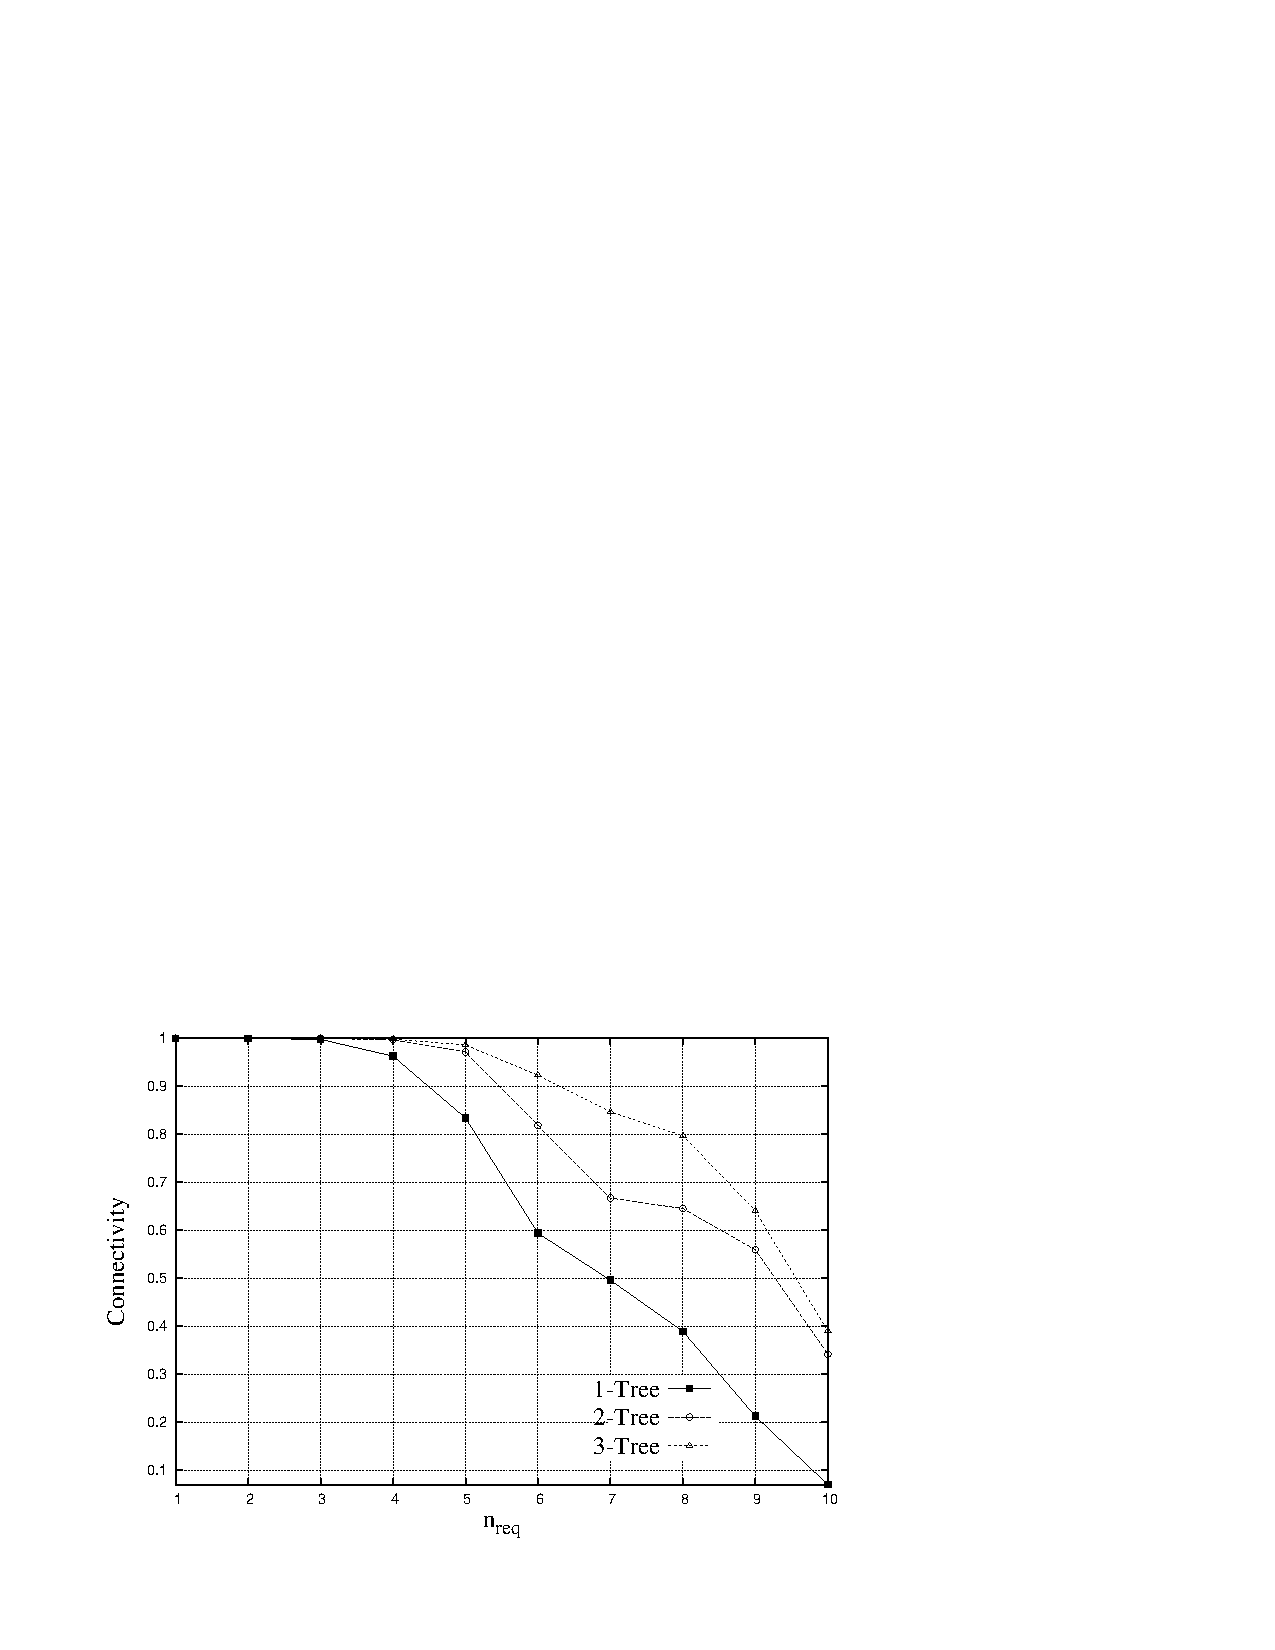
\includegraphics[width=2 in, height=1.5 in]{abc.pdf}
\caption{Connectivity versus $n_{req}$}
\label{Fig:CvCwr1}
\end{minipage}
\begin{minipage}{0.45\linewidth}
\centering
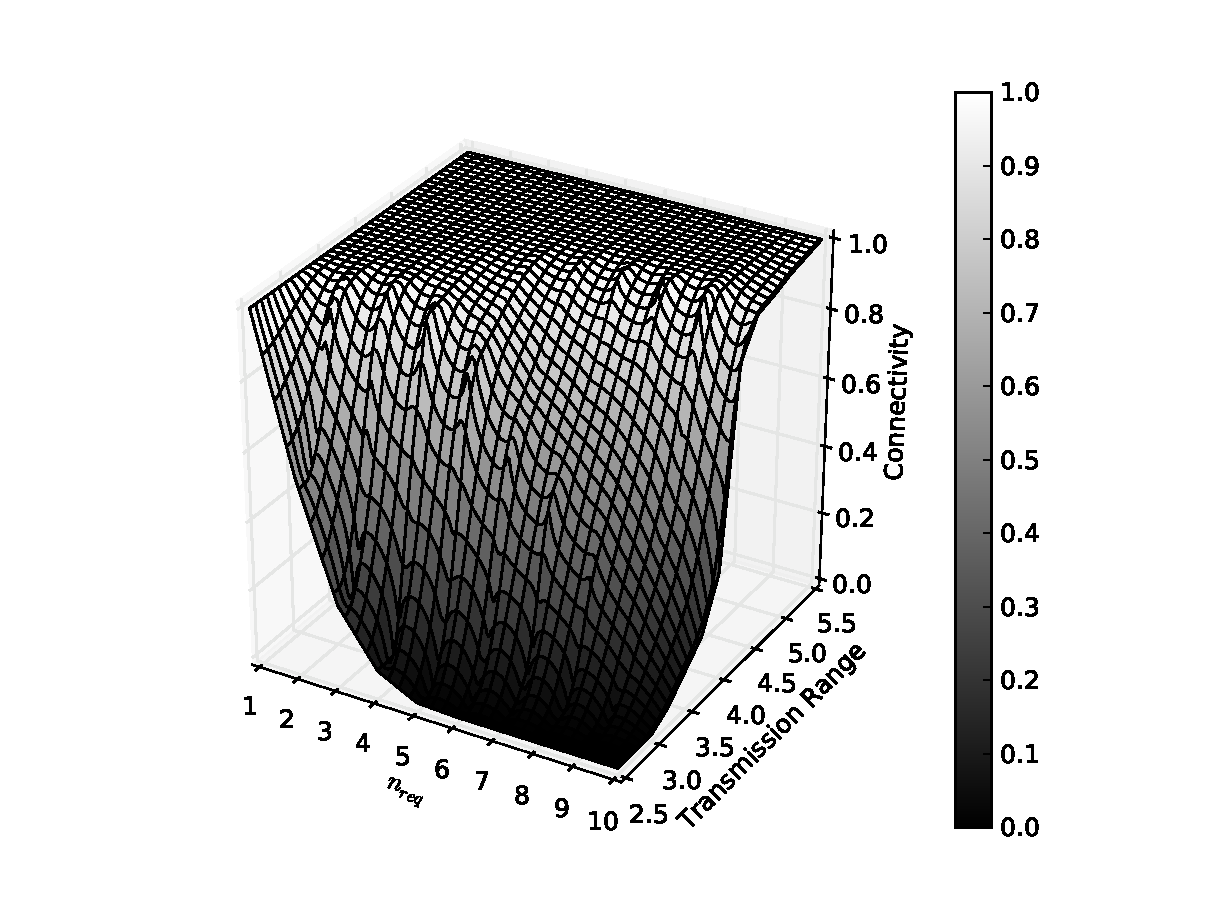
\includegraphics[width=2 in, height=1.5 in]{3D.pdf}
\caption{Connectivity versus $n_{req}$ and transmission range}
\label{Fig:CvCwr2}
\end{minipage}
\end{figure}

\end{frame}
%-----------------------------------------
%-----------------------------------------
\begin{frame}
\frametitle{Concluding Remarks}
\begin{itemize}
\item This thesis is motivated by recent interest in UWSNs as a platform for preforming many useful tasks. 
\item A challenge arises since sensor nodes incur small scale and large scale movements that can disrupt network connectivity.
\item  Thus, tools for quantifying the likelihood that a network remains completely or partially connected become of interest.

\item the thesis has formalized 4 probabilistic connectivity problems, denoted $\ACONN,$ $ \SCONN, \ARCONN, \mbox{ and } \SRCONN$. 
\item The obtained results show that all of the 4 problems admit polynomial time algorithms on $k$-trees (and their subgraph), for any fixed $k$.
\end{itemize}
\end{frame}
%-----------------------------------------
\section{Future Research Directions}
%-----------------------------------------
\begin{frame}
\frametitle{Future Research Directions}
\begin{itemize}
\item Investigating the applicability of our algorithm to some other classes of graph to be a worthwhile direction.

\item It is interesting to analyze the delays incurred in typical data collection rounds.
\item It is worthwhile to investigate area coverage assuming a probabilistic locality model of the nodes.
\end{itemize}

\end{frame}
%-----------------------------------------


%-----------------------------------------
\begin{frame}
\frametitle{}
\begin{center}
\Huge Thanks!
\end{center}

\end{frame}
%-----------------------------------------
\end{document} 